\documentclass[12pt]{report}
\usepackage[margin=1in]{geometry}
\usepackage[compact,raggedright]{titlesec}
\usepackage{setspace} % for single/doublespacing commands
\usepackage{graphicx} % including graphics
% \usepackage{sectsty} % sexy section headings
\usepackage{pdfpages} % including multipage pdfs
\usepackage[export]{adjustbox} % for graphic frames and center
\usepackage{siunitx}
\usepackage[numbered]{matlab-prettifier} % including matlab w/ syntax highlighting
\usepackage[T1]{fontenc} % prettier matlab font
\usepackage{xfrac} % more legible inline fractions (\sfrac)
\usepackage{lmodern} % font package for above
\usepackage{multicol} % multiple columns
\usepackage[justification=centering]{caption} % figure captions (force centering)
\usepackage{amsmath} % more math symbols and shit
\usepackage{enumitem} % add arguments for enumerate to change style
\usepackage{subcaption} % subfigures with list of figure support
% \usepackage{subfigure}
\usepackage{multirow}
\usepackage{mathtools}
\usepackage{booktabs}
\usepackage{color}
\usepackage{ulem}
\usepackage{blindtext}
\usepackage[numbers]{natbib}
\usepackage{contour}
\usepackage{tabularx}
\usepackage{circuitikz} % drawing fancy shit
\usepackage{cancel} % arrow and cross math cancel symbol
\usepackage{lineno}
\usepackage{framed}
\usepackage{amssymb} % special math symbols
\usepackage{listings}
\usepackage{array}
\usepackage{BOONDOX-cal} % fancy mathtype script
\usepackage{fancyhdr}
\usepackage{flowchart}
\usepackage{color, colortbl}
\usepackage{tocloft}
\usepackage{url}
\usepackage{etoolbox}
\usepackage[usestackEOL]{stackengine}
\usepackage{caption}
% \usepackage{hyperref}

\setlength{\parskip}{\baselineskip}%
\setlength{\parindent}{0pt}%

\setcounter{secnumdepth}{5}
\renewcommand{\bibname}{References}
\sisetup{output-exponent-marker=\ensuremath{\mathrm{e}}}
\newcommand{\PreserveBackslash}[1]{\let\temp=\\#1\let\\=\temp}
\newcolumntype{C}[1]{>{\PreserveBackslash\centering}p{#1}}
\newcolumntype{R}[1]{>{\PreserveBackslash\raggedleft}p{#1}}
\newcolumntype{L}[1]{>{\PreserveBackslash\raggedright}p{#1}}
\lstMakeShortInline[style=Matlab-editor]| % matlab inline escape character
\graphicspath{{images/}}
\renewcommand\thesection{\arabic{section}}
\renewcommand\labelitemi{---}
\lstset{numberstyle=\ttfamily\small\color{gray}}
\renewcommand\linenumberfont{\ttfamily\small\color{gray}}
\setlength\linenumbersep{6mm}
\hbadness=99999  % or any number >=10000
\apptocmd{\sloppy}{\hbadness 10000\relax}{}{}
\usetikzlibrary{arrows,calc,patterns,angles,quotes}
% \usetikzlibrary{shapes.geometric}
% \usetikzlibrary{decorations.pathmorphing,decorations.pathreplacing} % for snakes!
% \usetikzlibrary{positioning, circuits.logic.US}
\newcommand{\Lag}{\mathcal{L}} % lagrangian L

\apptocmd{\sloppy}{\hbadness 10000\relax}{}{}
\setlength{\cftbeforetoctitleskip}{-2em}
\setlength{\cftbeforeloftitleskip}{-2em}
\setlength{\cftbeforelottitleskip}{-2em}
% \allsectionsfont{\raggedright} % w/ secsty
\setlist[enumerate]{wide=0pt, widest=99,
                    leftmargin=\parindent,topsep=0pt,partopsep=0pt,
                    label=\thesubsubsection.\alph*,font=\itshape}

\newcommand{\hiddensubsection}[1]{
  \stepcounter{subsection}
  \subsection*{\arabic{section}.\arabic{subsection}\hspace{1em}{#1}}
}
\newcommand{\hiddenappsec}[1]{
  \stepcounter{section}
  \subsection*{\Alph{section}\hspace{1em}{#1}}
}
\newcommand{\hiddenappsub}[1]{
  \stepcounter{subsection}
  \subsection*{\Alph{section}.\Roman{subsection}\hspace{1em}{#1}}
}

\titlespacing\section{0pt}{0pt}{-5pt}
\titlespacing\subsection{0pt}{0pt}{-5pt}
\titlespacing\subsubsection{0pt}{0pt}{-5pt}

\AtBeginEnvironment{thebibliography}{\def\UrlFont{\normalfont\itshape}}

\DeclareCaptionFormat{cont}{#1 (cont.)#2#3\par}

\DeclareCaptionLabelFormat{r-parens}{Figure \thefigure#2:} %Define our custom label

% \captionsetup{font=footnotesize} % The general caption settings
\captionsetup[sub]{              % The subcaption settings
    labelformat=r-parens}        % Use our custom label format

% \renewcommand{\thesubfigure}{\thefigure\alph{subfigure}}
% \looseness=-1 % for one-liners bleeding off into the next page

\begin{document}
\normalem
\begin{titlepage}
\flushleft
\doublespacing
\Large
\textsc{Test Document} \\
\normalsize
Trey Dufrene, Zack Johnson, David Orcutt, Alan Wallingford, Ryan Warner
\vfill
\center
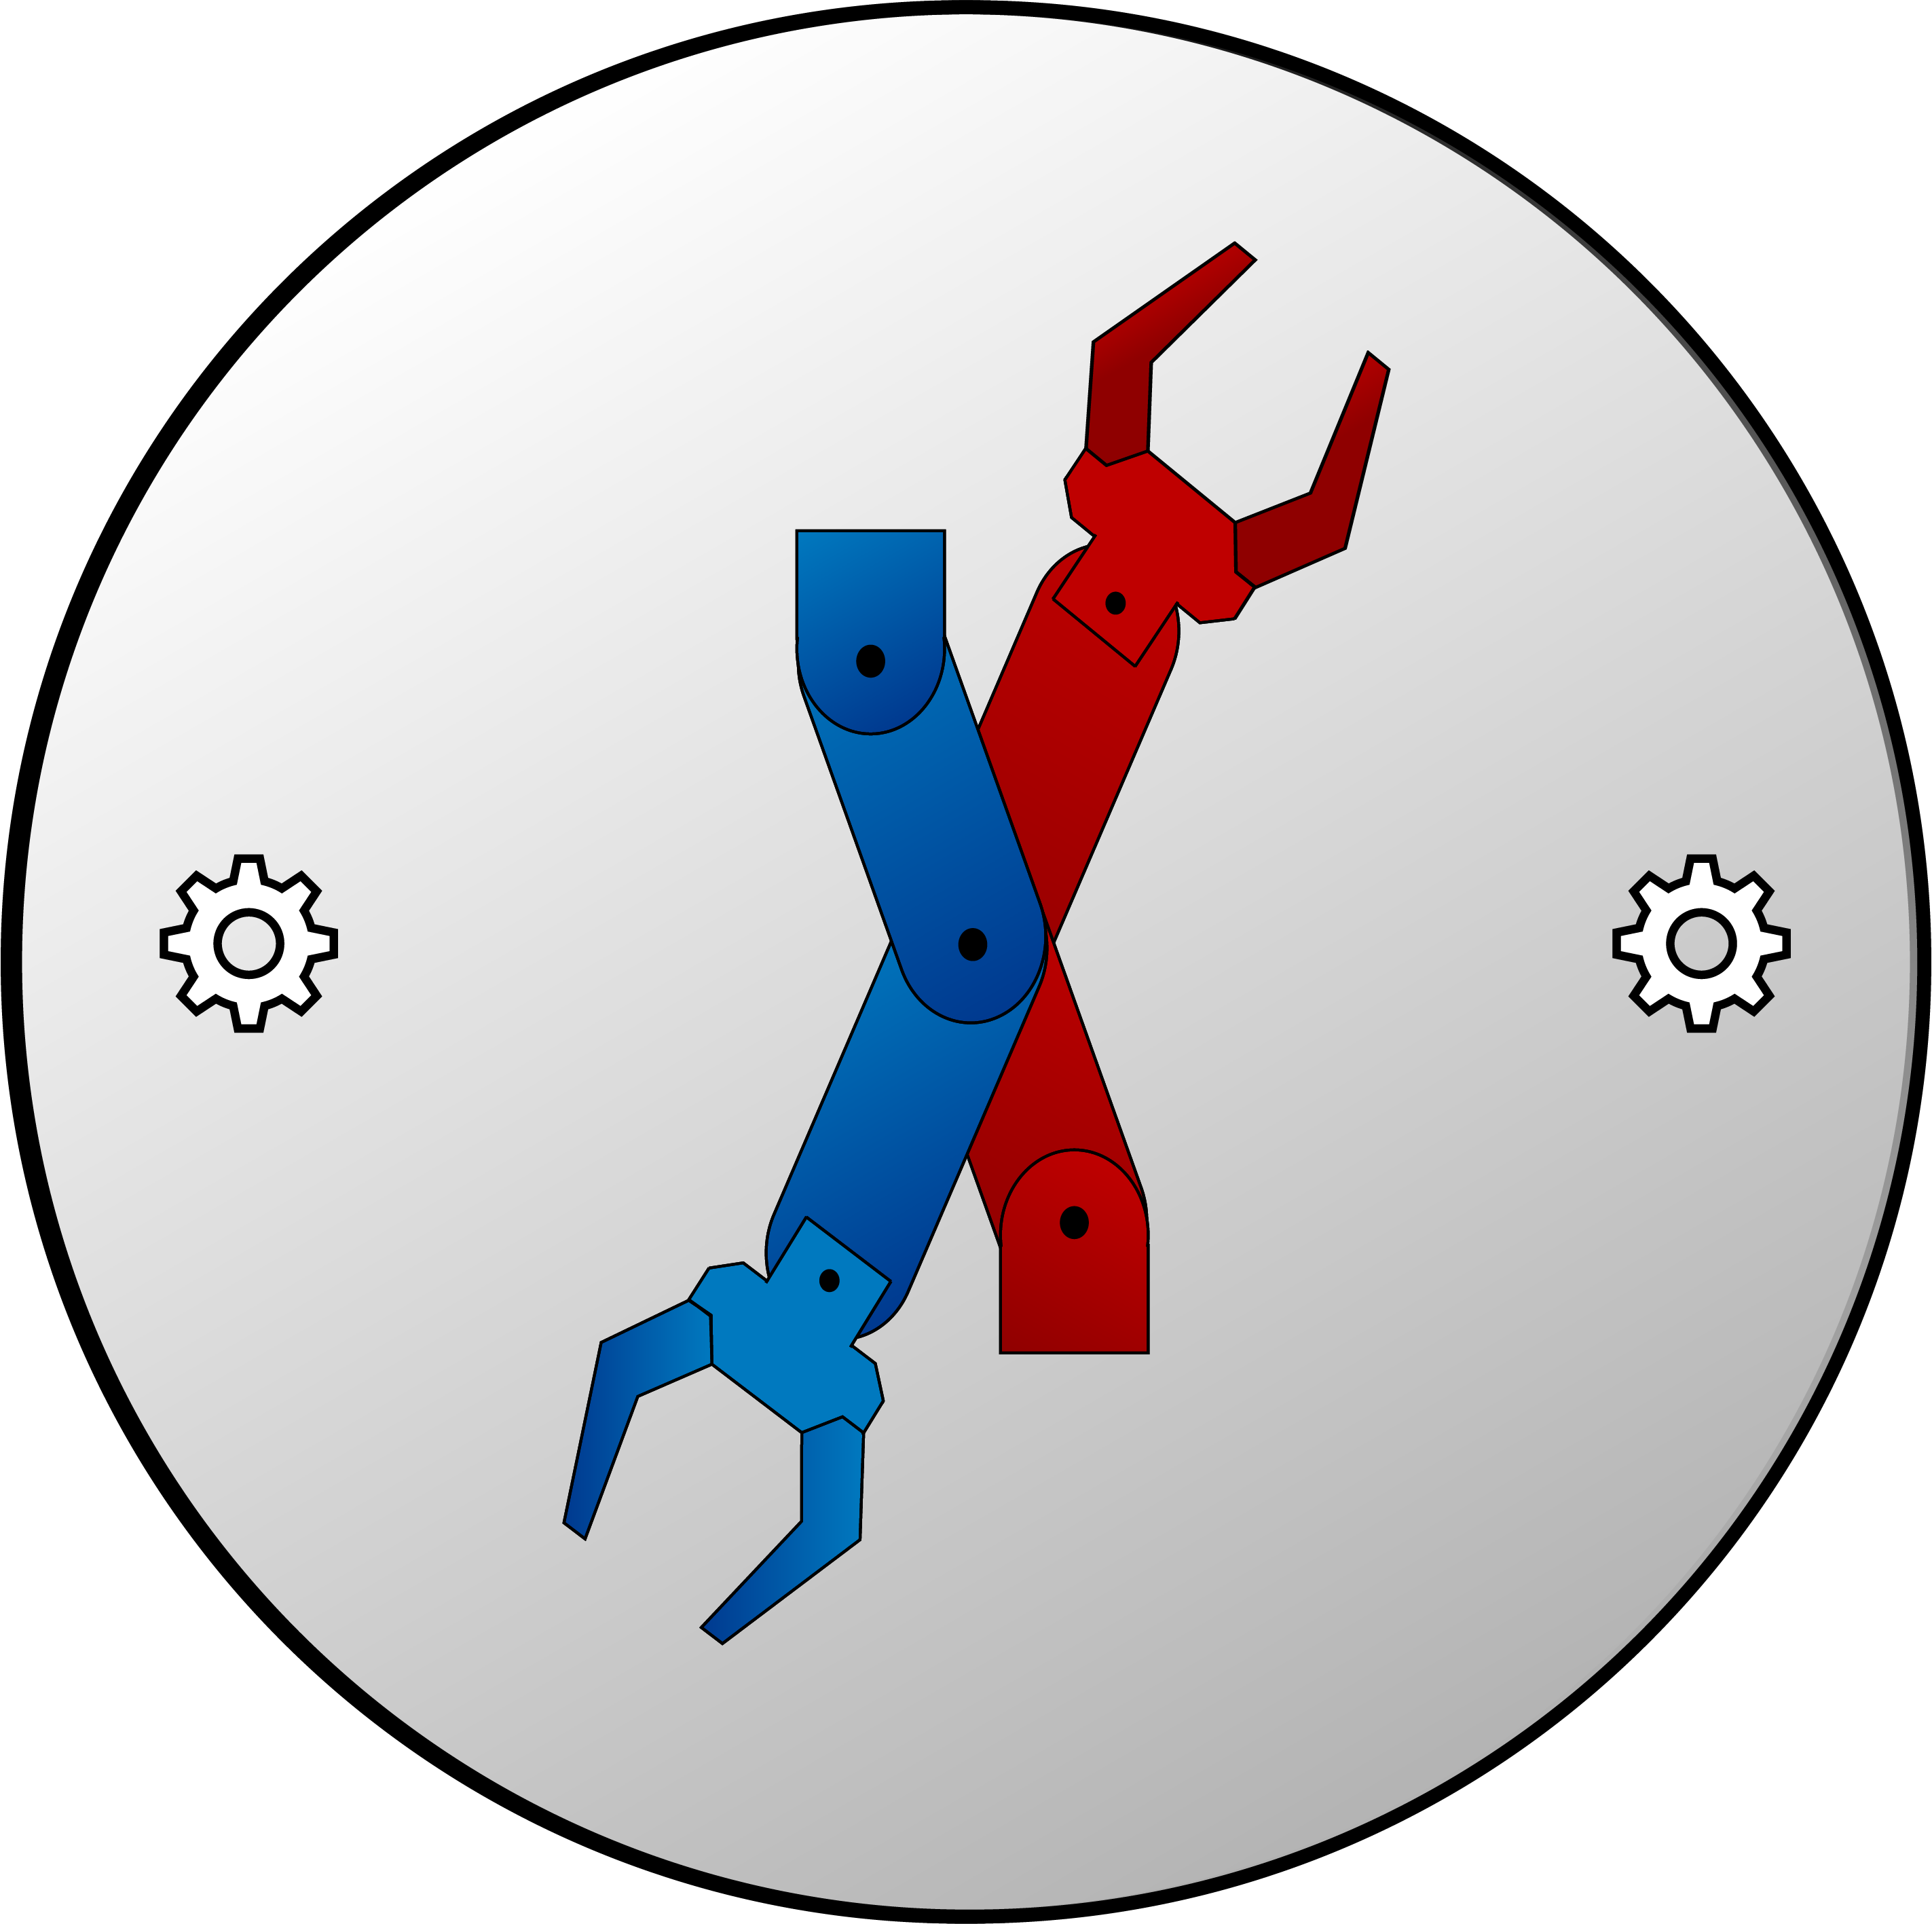
\includegraphics[width=.45\textwidth]{logo}
\vfill
\flushleft
ME 407 \\
Preliminary Design of Robotic Systems \\
Embry-Riddle Aeronautical University \\
\vspace{2ex}
\begin{minipage}[c]{.5\textwidth}
\flushleft

\includegraphics[width=.95\textwidth]{erau}
\end{minipage}%
\begin{minipage}[c]{.5\textwidth}
\flushright

\includegraphics[width=.8\textwidth]{text}
\end{minipage}
\end{titlepage}

\pagenumbering{roman}
\begin{abstract}
The Manipulator for Educational Institutions with Open Source Integrated Systems (MEIOSIS) aims to increase the accessibility of robotics to secondary educational institutions and hobbyists. Accordantly, the manipulator is 3D printed in PLA with aluminum tube supports and costs the end-user less than \$1000. The manipulator has six links and a base. The base houses a Raspberry Pi 3B and power supply. The Raspberry Pi controls seven Dynamixel smart servos with position feedback and proportional derivative control. Six MX-12W servos actuate six rotational joints, while one AX-12A servo actuates the removable end-effector. They provide the manipulator a position repeatability within 2mm of the previous pose. The manipulator can draw as well as perform pick and place operations within its dexterous workspace which is a hemispherical sub-shell of the reachable workspace of 280 mm thickness. The manipulator’s operation is controlled by open-source software.
\end{abstract}
% {\tableofcontents\let\clearpage\relax\listoffigures\let\clearpage\relax}
{\tableofcontents\clearpage\listoffigures\clearpage\listoftables}
\clearpage
\newpage
\section*{List Of Acronyms and Abbreviations}
\begin{tabular}{rcl}
  FK &:& Forward Kinematics \\
  IK &:& Inverse Kinematics  \\
  PD &:& Proportional Derivative \\
  % $k$~:& Spring constant \\
  % $h_{b}$~:& Distance to bar ($G$) from datum \\
  % $F_s$~:& Force onto bar due to spring\\
\end{tabular}

\section*{Notation}\vspace{-\baselineskip}
\renewcommand{\arraystretch}{2.25}
\begin{tabular}{rcl}
\large%
\(
{}^{\text{\scriptsize Frame}}_{\text{\scriptsize From}}~{r}~_{\text{\scriptsize To}}
\)\normalsize &:& Direction Vectors\\
\(
{}^{\text{\scriptsize From}}~{T}~_{\text{\scriptsize To}}
\)\normalsize &:& Direction Cosine (Transformation) Matrices \\
\(c_{\theta_{nm}}\)&:& \( \cos(\theta_n + \theta_m)\)\\
\(s_{\theta_{nm}}\)&:& \( \sin(\theta_n + \theta_m)\) \\
\end{tabular}
\renewcommand{\arraystretch}{1}
\newpage

\pagenumbering{arabic}
\section{Introduction}
The Rethink Robotics Sawyer manipulator retails for \$29,000 \cite{rr}. The Prescott Embry-Riddle robotics lab has 1 and the University's average student pays \$35,654 annually -- after financial aid \cite{ff}. Further, \$25,000 to \$35,000 is a common price for manipulators with a reach of approximately 1 meter and payload capacity below 1 kg \cite{gg}. While Trossen Robotics offers low cost manipulators between one sixth and one sixtieth of Sawyer’s cost, for accuracy of 1mm, the cost is still around \$2,000. For secondary education institutions, robotics is cost prohibitive. Consequently, students have less opportunities in high school to learn about robotics. The Manipulator for Educational Institutions with Open Source Integrated Systems (MEIOSIS) aims to increase the accessibility of robotics education to secondary education institutions and hobbyists.

In biology, meiosis is a process of cell division similar to mitosis. However, unlike mitosis, the resulting daughter cells are used to create new life during sexual recombination. Meiosis occurs in two sets of cell division: meiosis I and meiosis II. Analogously, MEIOSIS has a Preliminary and Detail semester. During meiosis I, chromosomes pair up and swap genetic material (DNA) in preparation for cell division. Then, during meiosis II, the parent cell splits into two haploids, which each split into two gametes. The gamete cells have half the number of chromosomes compared to a cell produced by mitosis and are not identical to their parent cell. When combined with another gamete, a new, unique cell emerges. MEIOSIS does not change the DNA of robotics. However, in combining with user needs and incorporating innovative design elements, MEIOSIS brings new life to robotics education.

This document outlines MEIOSIS’s solution for increasing the accessibility of robotics education, current project status, and plans for the Detail semester. Specifically, it is subdivided into four sections: Requirements, Conceptual Design, Specifications, and Preliminary Design. The Preliminary Design comprises the majority of the document. It explains the evolution of MEIOSIS’s manipulator, noting design decisions and changes made from simulations, tested parts, and motor calculations. Finally, an appendix contains simulation code and drawings for all parts.


\section{Requirements}
The requirements of the system concisely define the capabilities the system must possess in order to solve the stated problem.
\hiddensubsection{Hardware}
The following requirements are hardware specific and dictate the physical constraints the system must adhere to.
\subsubsection{The system shall cost the end-user no more than \$1000.}
\subsubsection{The system shall be fully dexterous without being kinematically redundant.}
To create a system with the intention of advancing education, it must be complex enough to encourage higher level problem solving, as well as be capable enough (dexterous) in a broad spectrum of tasks — in the interest of remaining useful in addition to retaining the interest of students.

\subsubsection{The system end effector shall maintain a positional accuracy magnitude of \(\pm 1\) mm and an orientation accuracy of \(\pm 5^{\circ}\) eigen angle from the base frame.}
To ensure that the robot has educational value, the accuracy must be defined so that any desired positions and movements are achieved.

\subsubsection{The system end effector shall maintain a pose repeatability magnitude between 0.1—1.5 mm for the position and \(\pm 4^{\circ}\) eigen angle from the base frame for the orientation.}
This is to ensure a robot that can execute the same movement commands repeatedly and have the same results every time.

\subsubsection{The system’s reachable workspace shall be a hemisphere with a radius of 300-700 mm.}
This workspace will provide enough movement to manipulate objects in order to perform basic tasks.

\subsubsection{The system’s dexterous workspace shall contain a hemispherical shell within the reachable workspace with a thickness of 280 mm.}

\subsubsection{The system shall have a removable end effector capable of picking and placing a low-odor chisel tip Expo dry erase marker.}
This creates a robot capable of performing a variety of basic tasks, which enhances its educational value.

\subsubsection{The system shall be able to write with a low-odor chisel tip Expo dry erase marker.}

\hiddensubsection{Software}
\subsubsection{The system shall be open source.}
This will create an easily obtainable, low cost method of distributing the system’s source code, which may be modified for personal use.

\subsubsection{The system shall be capable of operating given only desired end effector cartesian coordinates specified with respect to the base frame.}
This simplicity makes the system of use to inexperienced users.

\newpage
\section{Conceptual Design}
The terminator T-2000 is a science-fiction spectacle of a robot -- until you see the price. Channeling the inspiration many high school students may have for robotics, MEIOSIS robotics aims to provide an affordable manipulator to educators and enthusiasts. MEIOSIS uses primarily 3-D printed components and easily accessible materials. Among these materials are a Raspberry PI, smart servos and metal tubing. These features create an open-source manipulator accessible to the public to further robotics education.
\hiddensubsection{Physical System Overview}
The physical design of the robotic manipulator is shown in Figures \emph{\ref{fig:overall}, \ref{fig:base}, \ref{fig:link1},} and \emph{\ref{fig:link2}}.

\begin{figure}[htp]
  \centering
  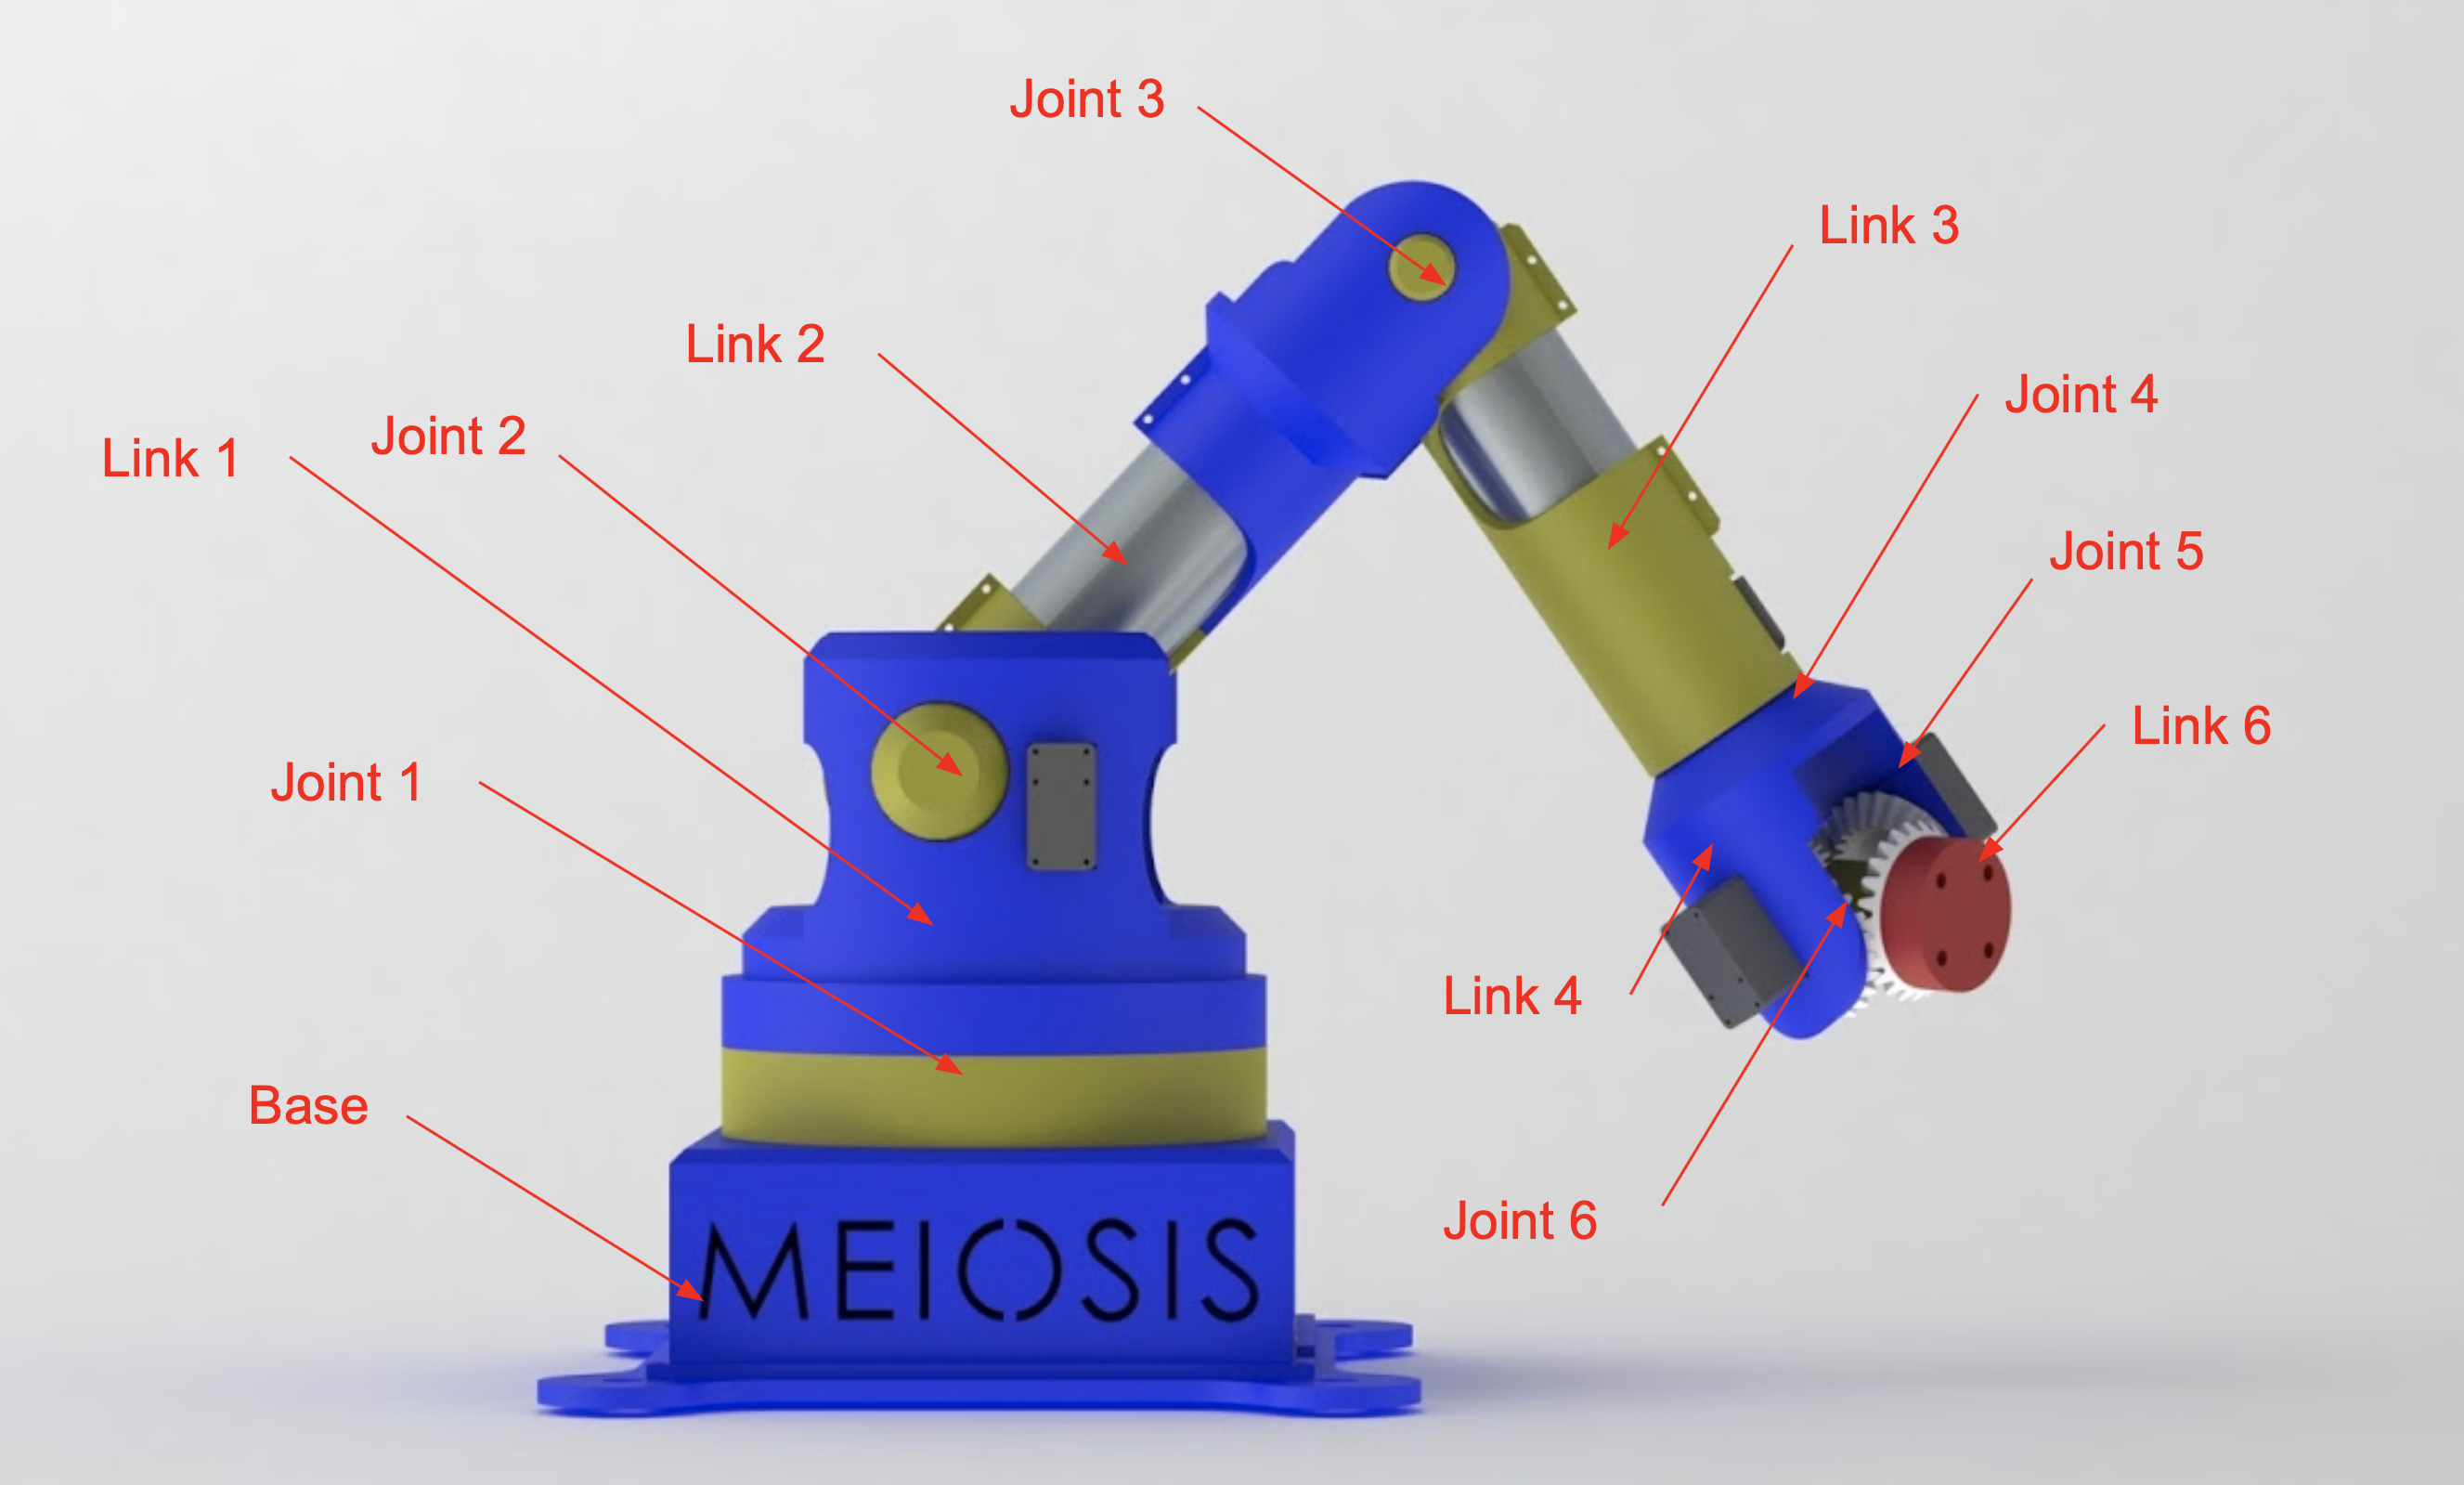
\includegraphics[frame, width=.75\textwidth]{overall_render}
  \caption{Overall System Conceptual Design }
  \label{fig:overall}
\end{figure}

The colored links in \emph{Figure \ref{fig:overall}} distinguish the different joints and links of the manipulator. The overall reach of the robot is 582.5 mm. This length was chosen to decrease material cost and weight while still satisfying requirement 2.1.2 and 2.1.5, allowing the manipulating to pick and place objects to perform basic tasks. The base of the robot is made to contain the Raspberry Pi and other electrical components.

\subsubsection{Base}
The base of the manipulator will house several of the electronic components, such as the computational system, power supply, and motor controller. A cross section of the base can be seen in \emph{Figure \ref{fig:base}}.
\begin{figure}[htp]
  \centering
  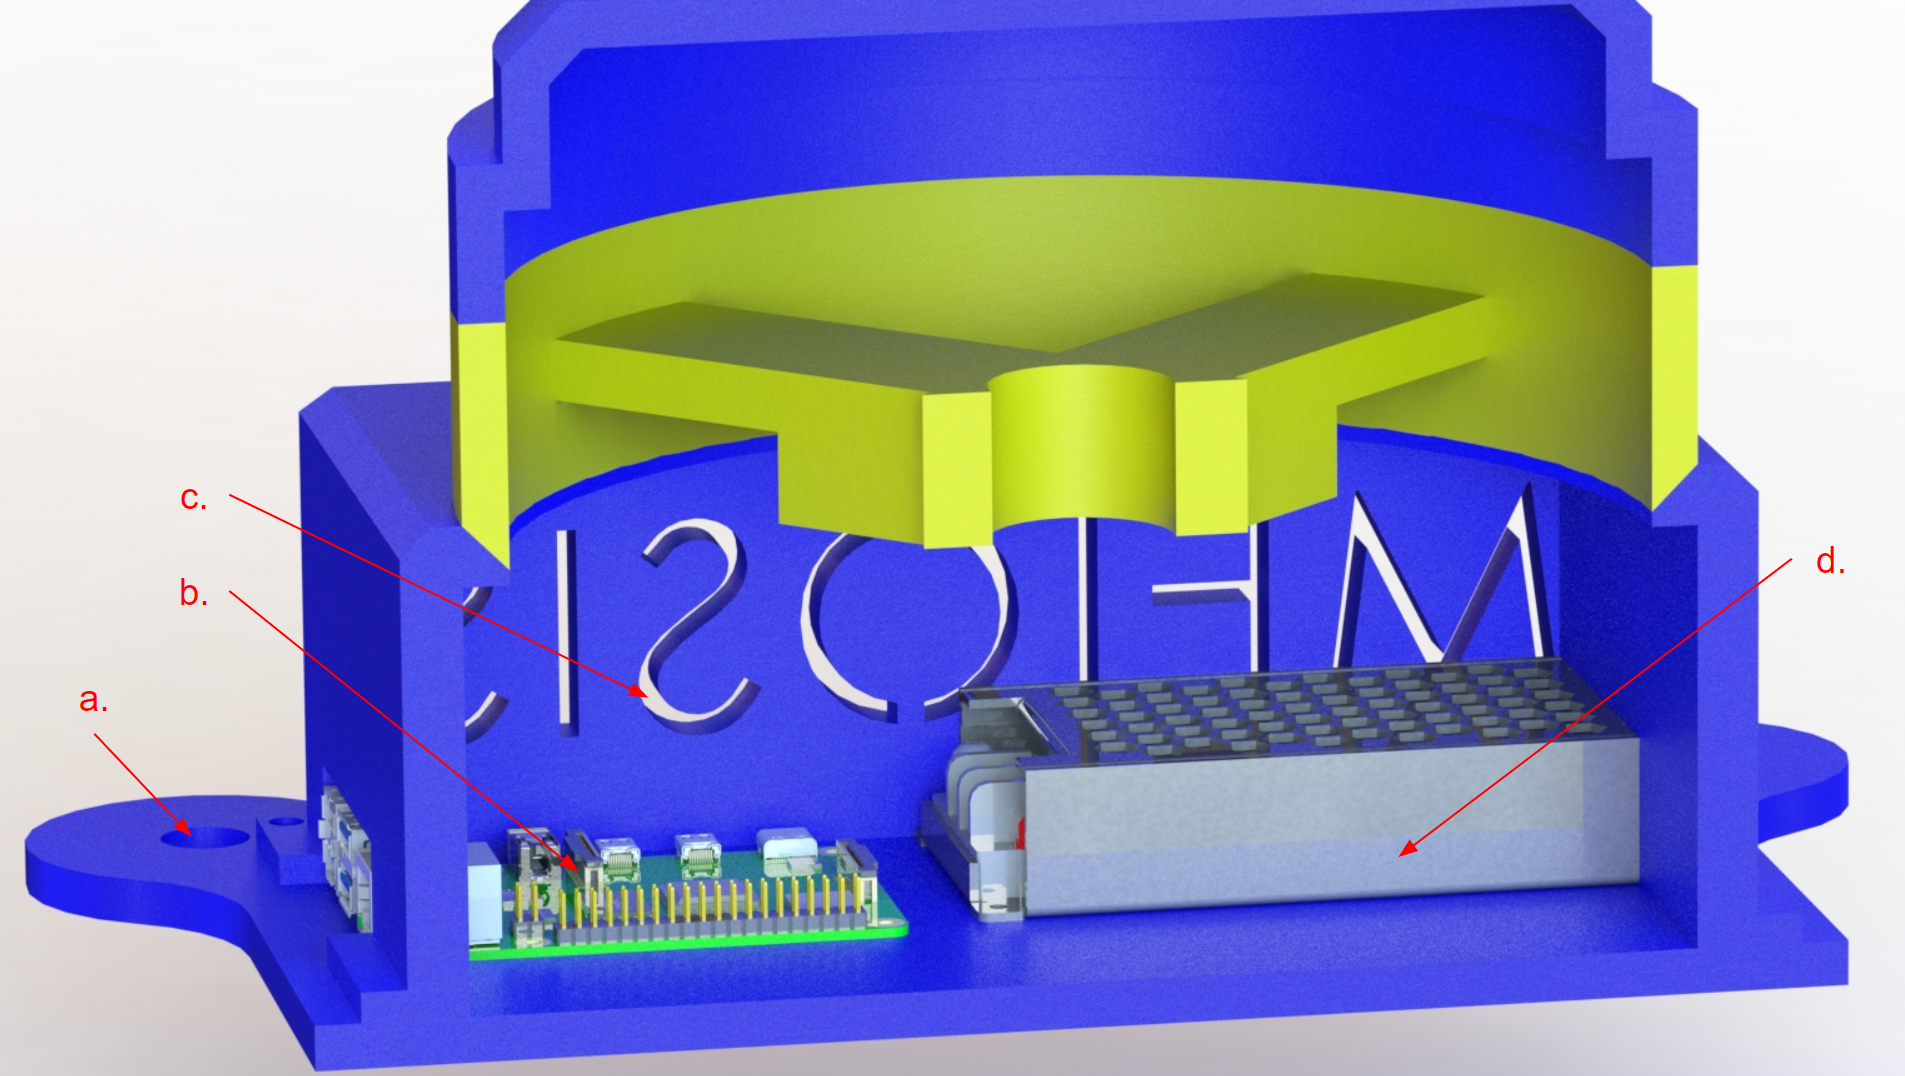
\includegraphics[frame, width=.75\textwidth]{base_callouts}
  \caption{Manipulator Base with Call-outs}
  \label{fig:base}
\end{figure}

From \emph{Figure \ref{fig:base}},
\begin{enumerate}[label=\alph*.]
  \item \emph{Base Supports:}
  The base supports are located at each corner of the base and allow the base of the manipulator to be securely attached to a variety of surfaces with either standard fasteners or suction cups.
  \item \emph{Computational System:}
  The computational system is a Raspberry Pi; it is housed in the base, which allows the Raspberry Pi to be more easily accessible. The primary reason for this system being chosen is to fulfill the budget requirement, 2.1.1. The Raspberry Pi computes the manipulator's inverse kinematics and sends the angle commands to the servos.
  \item \emph{Airflow Cutouts:}
  The side of the base hsd cutouts to allow for airflow through the base; since the power supply is housed inside of the base as well as the computational system, the temperature must be regulated to prevent overheating.
  \item \emph{Power Supply:}
  The power supply is housed in the base as well, which allows the power supply to be more accessible and therefore more modifiable, so the end-user can easily expand the system to fulfill their needs.
\end{enumerate}
\newpage
\subsubsection{Links}
\emph{Figure \ref{fig:link1}} shows the links and their key features.\\
\begin{figure}[htp]
  \centering
  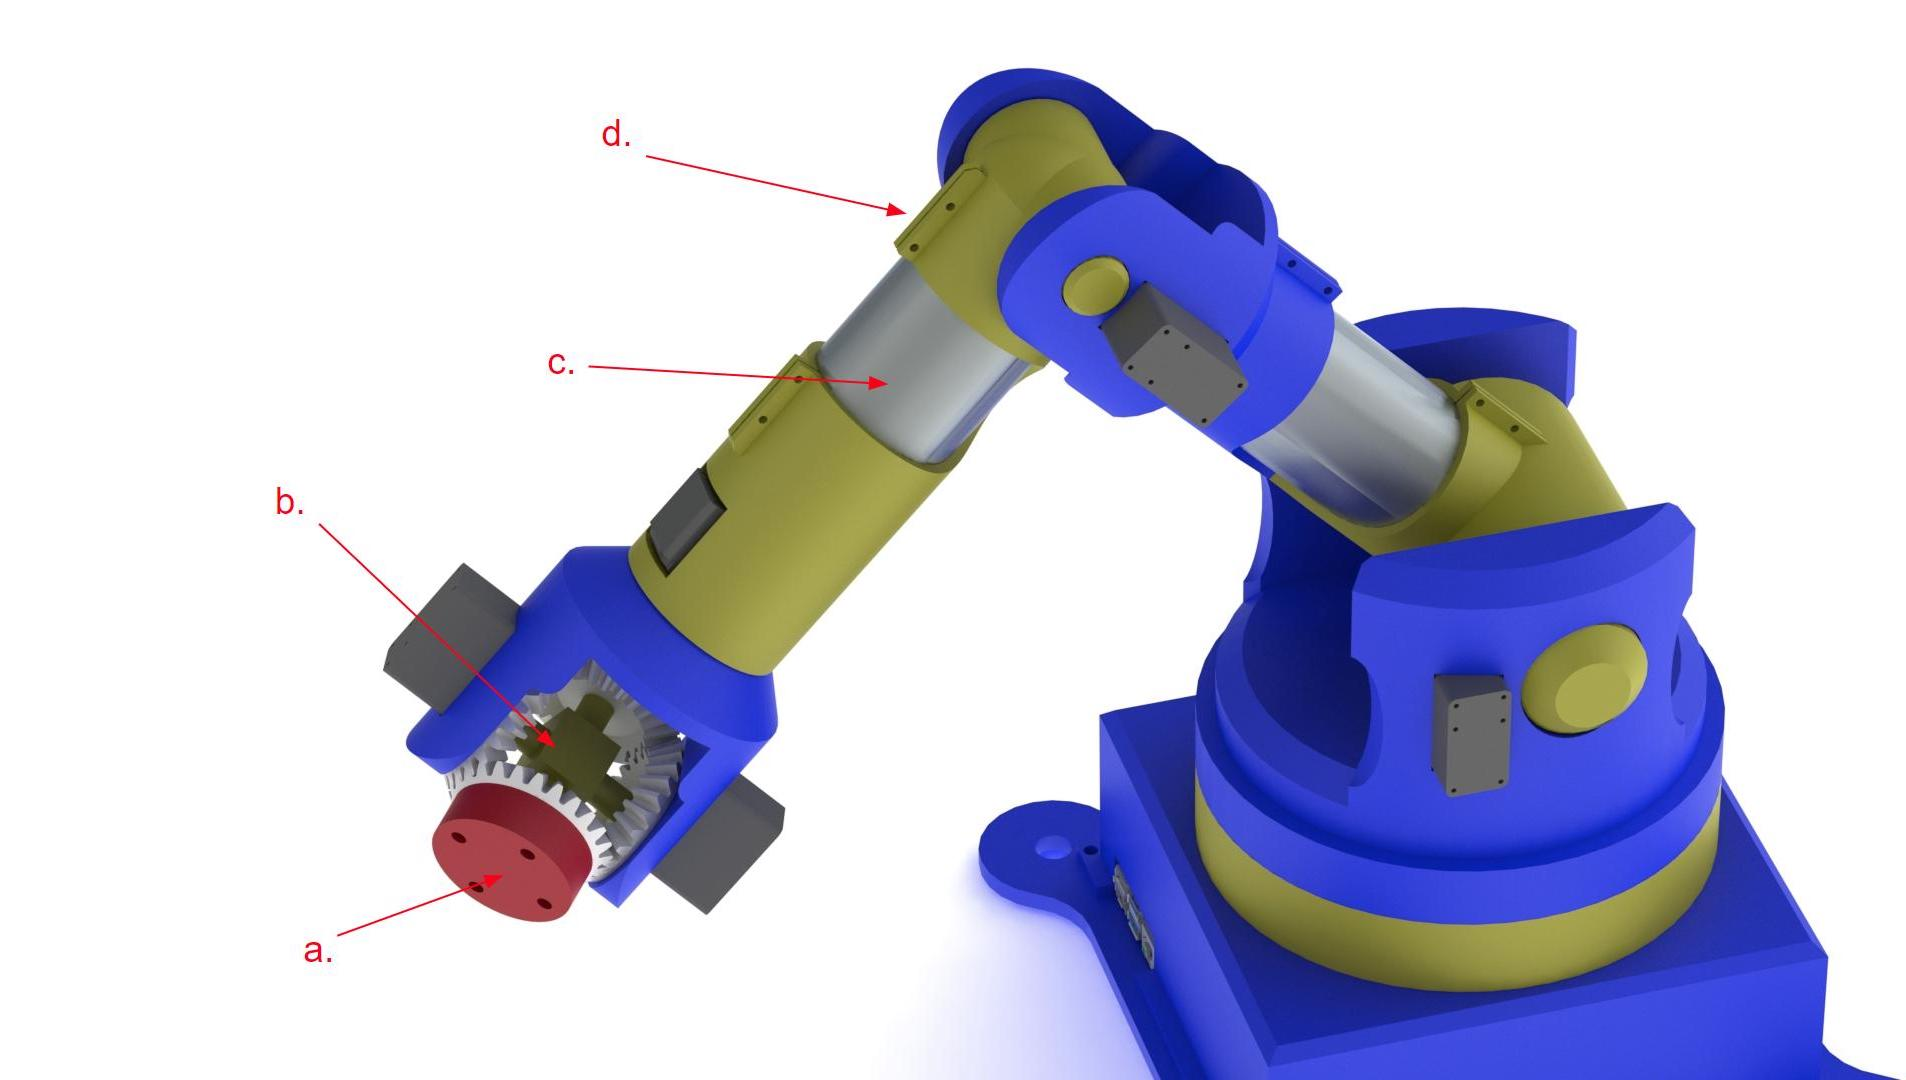
\includegraphics[frame,width=.63\textwidth]{link_callouts}
  \caption{Drawing Showing Key Features of Design}
  \label{fig:link1}
\end{figure} \\
In \emph{Figure \ref{fig:link1}}, call-out (a) shows the connection point for the end effector. The mounting layout is the standard used by the Sawyer manipulator. The end effector mounting layout may be adjusted to accommodate lower cost, more accessible end effectors. Call-out (b) shows the differential gearbox that is used in the manipulator’s wrist, saving space and weight. The manipulator has aluminum tubing as support in the links (c) and are attached to the 3D printed portion of the robot using clamp joints (d) tightened by screws.

\emph{Figure \ref{fig:link2}} depicts the cross section of link 2 for the manipulator.
\begin{figure}[htp]
  \centering
  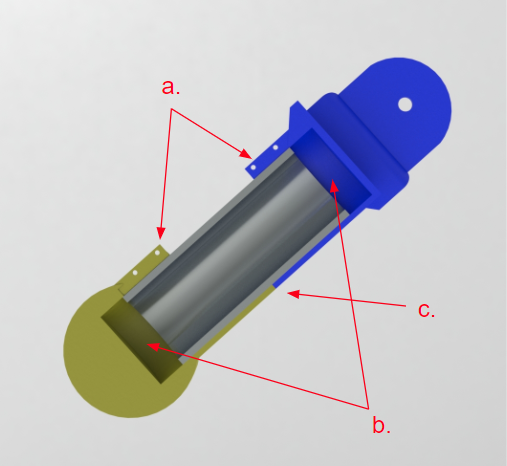
\includegraphics[frame,width=.35\textwidth]{link_cross_section}
  \caption{Drawing Showing Link Cross Section}
  \label{fig:link2}
\end{figure}

The cross section seen in \emph{Figure \ref{fig:link2}} shows the internal design for links two and three. It features two clamps that hold a hollow aluminum bar in place (a) and allows for gaps between the aluminum tube and the 3D printed call-out (b). The proper length is dictated by the 3D printed guides lining up at call-out (c). This design allows for imprecision in the manufacturing of the aluminum tube.

\hiddensubsection{System Functions}
The system can be divided into two subsystems: the electrical and software systems. The electrical subsystem includes the wiring and hardware computational components, power system, actuators with drivers, and sensors. The software subsystem includes the algorithm for the computational system.
\hiddensubsection{Electrical}
\emph{Figure \ref{fig:eblock}} is the block diagram for the electrical system of the manipulator.

\begin{figure}[htp]
  \centering
  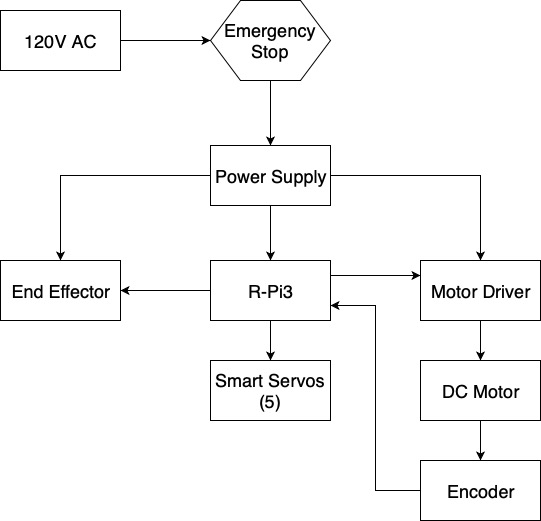
\includegraphics[width=.55\textwidth]{eblock}
  \caption{Electrical System Block Diagram}
  \label{fig:eblock}
\end{figure}

\emph{Figure \ref{fig:eblock}} shows that the electrical systems of the manipulator consists of three main components: the power supply, the Raspberry Pi, and the servos. Power is supplied by the 120V AC from standard wall outlets. A power supply converts the AC voltage to the required voltages for each component. One component is the Raspberry Pi, which performs calculations for motor control. The Raspberry Pi sends signals to the DC motor driver and the five smart servos. The smart servos have an on-board controller, so no feedback will be necessary. However, the first joint, between the base and the first link, is actuated by a DC motor with an encoder to minimize cost.

\hiddensubsection{Software}
\emph{Figure \ref{fig:sblock}} shows the software flowchart for the system.
\begin{figure}[ht]
  \centering
  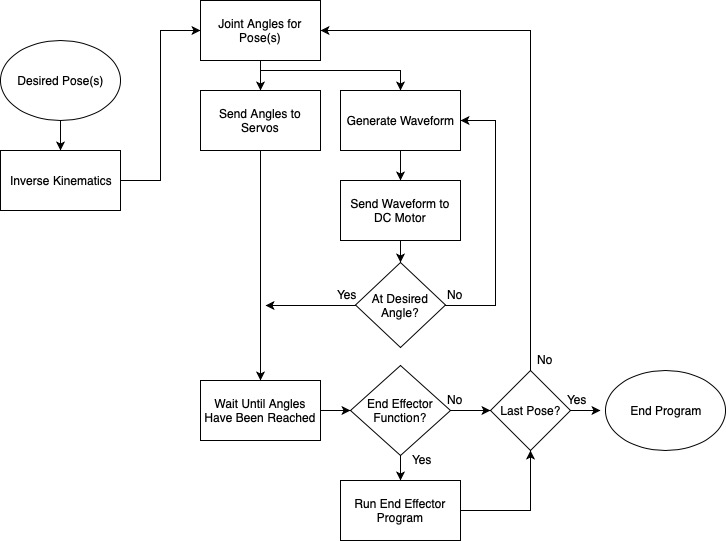
\includegraphics[width=.85\textwidth]{sblock}
  \caption{Software Flowchart}
  \label{fig:sblock}
\end{figure}

\emph{Figure \ref{fig:sblock}} shows that the software receives the desired pose or poses that the user would like the manipulator to reach. Next, the Raspberry Pi uses inverse kinematics to calculate the necessary joint angles. The wave-forms/desired angles are sent to the respective drivers/motors, and positional information is be sent back to the Raspberry Pi to adjust the DC motor angle. When the motors have reached their desired pose, the Raspberry Pi actuates the end effector if it is specified by the user. The system then checks to see if there are any more poses to reach and either repeats the steps in the motor control section given the desired angles of the new pose or ends the program if the last pose has been reached.

\hiddensubsection{Decision Matrices}

Each team member’s conceptual design provides a variety of different options for select issues, and in order to narrow down the options into the best choice decision matrices are used to make unobjective decisions about each individual topic. The weights of each criteria are defined by the average of our votes on how important the criteria is on a scale of one to ten. The same method is used to rate the different options on each criteria. The most important decision that needs to be made is what configuration the manipulator will have as the configuration has an affect on almost all the design choices. There are five potential configurations, and the scores of each option can be seen in \emph{Table \ref{table:manip}}.

\begin{table}[htp]
  \center
  \caption{Configuration Decision Matrix}
  \label{table:manip}
\begin{tabular}{C{3cm}|c@{\hskip 3pt}C{2.5cm}C{2cm}@{\hskip 3pt}C{2cm}@{\hskip 3pt}C{3cm}@{\hskip 3pt}c@{\hskip 3pt}}
\multirow{2}{*}{\textbf{Configuration}} & \multirow{2}{*}{\textbf{Cost}} & \textbf{Educational Value} & \textbf{Ease of Use} &
\textbf{Ease to Program} & \textbf{Ease of Manufacture} & \multirow{2}{*}{\textbf{Total}} \\
\textbf{Weighting} & 10 & 8 & 7 & 2 & 6 & \\\hline
Cartesian w/ Spherical Wrist & \multirow{2}{*}{5} & \multirow{2}{*}{9} & \multirow{2}{*}{10} & \multirow{2}{*}{8} & \multirow{2}{*}{4} & \multirow{2}{*}{232} \\
RRR w/ Spherical Wrist & \multirow{2}{*}{8} & \multirow{2}{*}{9} & \multirow{2}{*}{7} & \multirow{2}{*}{7} & \multirow{2}{*}{8} & \multirow{2}{*}{\textbf{263}} \\
Cylindrical & 7 & 10 & 7 & 8 & 7 & 257 \\
SCARA & 6 & 9 & 8 & 8 & 6 & 240 \\
Spherical & 7 & 10 & 7 & 7 & 6 & 249 \\
\end{tabular}
\end{table}

The results from \emph{Table \ref{table:manip}} show that the solely rotational configuration is the best option, followed closely by the cylindrical. Having translational joints is too be problematic for manufacturing and more expensive, and that is enough of an issue that the rotational manipulator has the advantage over the rest of the options.

Another design choice that needs to be made is what material the manipulator will be constructed out of. The main choices are to 3D print everything, manufacture the manipulator out of aluminum, or use a combination of the two. Cost and accessibility are the two highest weighted criteria as we deem them to be the most important aspects, followed by weight and manufacturability. Durability has the lowest weight because the manipulator should not have enough forces acting on it so that the strength of PLA compared to aluminum should not necessarily affect the manipulator. The grades of each material are shown in \emph{Table \ref{table:mat}}.

\begin{table}[htp]
  \center
  \caption{Material Choice Decision Matrix}
  \label{table:mat}
\small\begin{tabular}{c|cccccc}
\textbf{Material} & \textbf{Cost} & \textbf{Weight} & \textbf{Accessibility} & \textbf{Manufacturability} & \textbf{Durability} & \textbf{Total} \\\normalsize
Weighting & 9.2 & 6.6 & 8 & 6.4 & 5.4 & \\\hline
3D Printed & 8 & 9 & 8 & 9.4 & 5 & 284.16 \\
Aluminum & 4 & 5.8 & 5.8 & 6.6 & 9.2 & 213.4 \\
Combination & 8 & 7.8 & 7 & 9 & 9.2 & \textbf{288.36} \\
\end{tabular}
\end{table}

As seen in \emph{Table \ref{table:mat}}, the winning material is a combination of 3D printing and aluminum. The combination allows the manipulator to have 3D printed parts that would be hard to manufacture out of aluminum or that would not necessarily need to be extremely durable, and allows the use of aluminum for the aspects of the manipulator that need to be strong and durable. This option allows for the best aspects of both materials to be utilized.

The internal computing system for the manipulator is another decision that needs to be made, so another decision matrix is used to decide from the six options available. Because the manipulator is intended to be low cost and used by primary education institutions, cost and ease of use are the two highest weighted criteria. Having a lot of capabilities and being able to function independently are factored in, but are deemed of secondary importance which can be seen in \emph{Table \ref{table:comp}}.

\begin{table}[htp]
  \center
  \caption{Computing Choice Decision Matrix}
  \label{table:comp}
\begin{tabular}{c|ccccc}
\textbf{Computing System} & \textbf{Cost} & \textbf{Capabilities} & \textbf{Ease of Use} & \textbf{Independence} & \textbf{Total} \\
Weights & 10 & 4.2 & 7.6 & 4.2 & \\ \hline
RPi & 7.9 & 6 & 9 & 10 & \textbf{214.6} \\
Jetson & 1 & 7 & 7 & 9 & 130.4 \\
RPi + Arduino & 4.8 & 7 & 8 & 10 & 180.2 \\
Arduino & 9 & 4 & 9 & 3 & 187.8 \\
B Black & 1.2 & 7 & 7 & 10 & 136.6 \\
B Green & 5 & 7 & 6 & 9 & 162.8 \\
\end{tabular}
\end{table}

\emph{Table \ref{table:comp}} shows that the Raspberry Pi is the winner by a significant margin, with only the Arduino coming close to it. While the Pi is not the most capable, its cost is very good and its ease of use and ability to independant functionality edge it over the other more capable competition. The arduino is the most cost effective, but its lack of functionality and low independence are detrimental to its score.

One of the other designs that needs to be selected was the way that the end effectors are attached to the end of the manipulator, and the different categories that are used to grade each option are ease of use, manufacturability, and durability, as seen in \emph{Table \ref{table:ee}}.

\begin{table}[htp]
  \center
  \caption{End Effector Attachment Design Decision Matrix}
  \label{table:ee}
\begin{tabular}{C{3.5cm}|cccc}
\textbf{EE Attachment} & \textbf{Ease of Use} & \textbf{Manufacturability} & \textbf{Durability} & \textbf{Total} \\
Weighting & 3.6 & 5 & 7 & \\\hline
Screw Connections & 6.8 & 8.8 & 9.8 & \textbf{137.08} \\
Snap Fit Joint & 8.6 & 5 & 2.2 & 71.36 \\
Threaded End Effector & 6.3 & 5.4 & 7.3 & 100.78 \\
\end{tabular}
\end{table}

From \emph{Table \ref{table:ee}}, the optimal design turns out to be screw connections in the end effector. The snap fit joint would be easier to use, but to create a functional snap fit connection would be difficult and would likely not be too durable. The threaded end effector is difficult to manufacture and not durable as well, so having connections for screw on the end effector is the clear choice.

\newpage
\section{Specifications}
% \hiddensubsection{Introduction}
% \label{sec:intro}
With the intention of making robotics education more accessible, The Manipulator for Educational Institutions with Open Source Integrated Systems (MEIOSIS) intends to provide high school educators and robot enthusiasts with a low cost manipulator. The system should be usable by novice students. It should also be modifiable to create a sustainably increased understanding of robotics. While MEIOSIS may not fully emulate industrial manipulators, it aims to provide more students with access to robotics education. \\
\begin{figure}[htp]
  \centering
  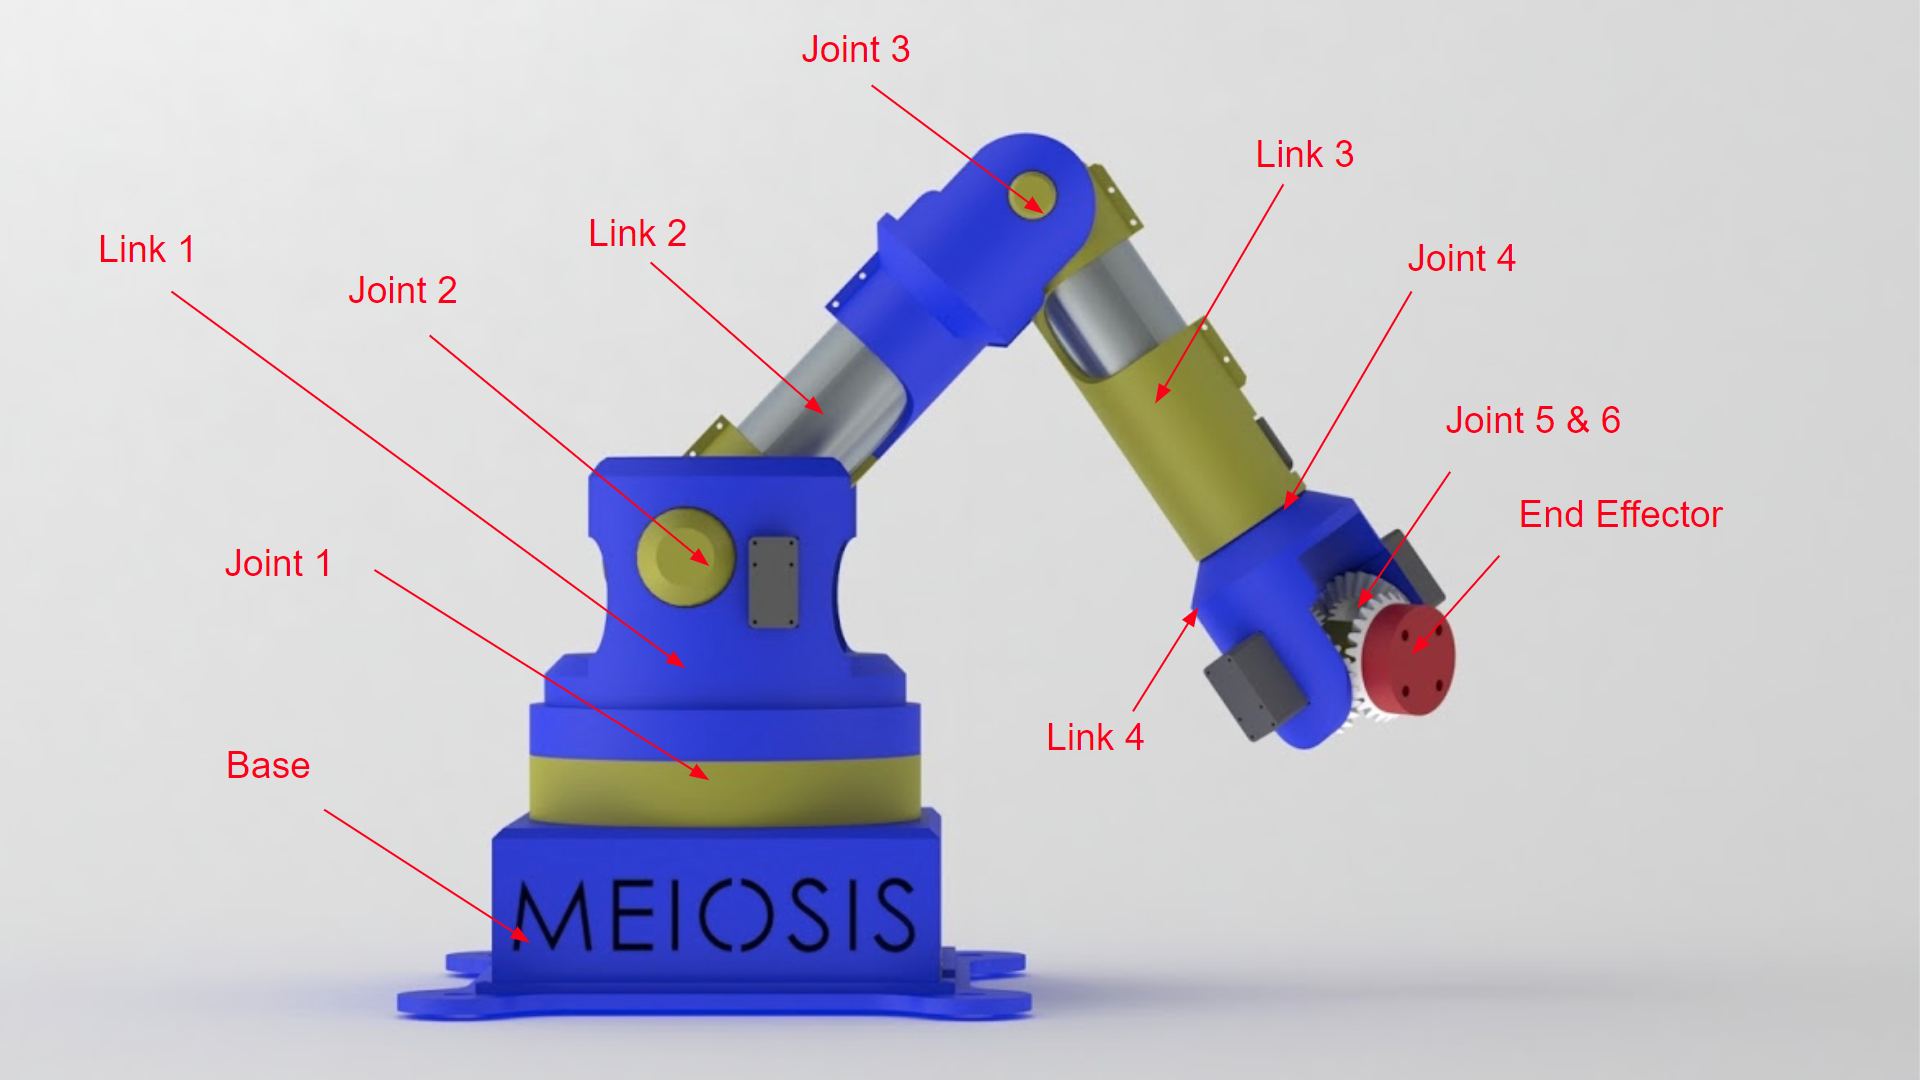
\includegraphics[frame,width=.75\textwidth]{model}
  \caption{Overview of Physical System}
  \label{fig:model}
\end{figure}
\newline
The design seen in \emph{Figure \ref{fig:model}} is based on our conceptual design. It features four links and six joints for rotation and will be referenced throughout this document. The base of the manipulator and end-effector can also be seen in the figure.
\hiddensubsection{Design Requirements}
The specifications of the system are strictly based on the requirements defined previously. The requirements are divided into two primary categories, hardware and software.
\vspace{-\baselineskip}
\hiddensubsection{Hardware}
The following requirements and specifications are hardware specific and dictate the physical constaints the system must adhere to.
\vspace{-\baselineskip}
\subsubsection{The system shall cost the end-user no more than \$1000.}
\begin{enumerate}
  \item \textit{The cost for the MEIOSIS team to develop the manipulator shall cost no more than \$800.}
\end{enumerate}
\subsubsection{The system shall be fully dexterous without being kinematically redundant.}
\begin{enumerate}
\item \textit{The system shall consist of six rotational joints connected by four links. The last three joints will create a spherical wrist.}
\end{enumerate}
As defined \cite{robo}, “A manipulator having more than six DOF is referred to as a kinematically redundant manipulator (5).” A manipulator with less than six degrees of freedom will not be fully dexterous within it's workspace. \emph{Figure \ref{fig:zero}} (see subsection \ref{sec:zero}, p. \pageref{fig:zero}) shows a six degree-of-freedom rotary manipulator with it's coordinate frames in zeroed positions. The joint and link locations are seen in \emph{Figure \ref{fig:model}} (see section \ref{sec:intro}, p. \pageref{sec:intro}).
\begin{enumerate}[resume]
\item \textit{The system shall have no link offsets.}
\end{enumerate}%
Link offsets as seen in \emph{Figure \ref{fig:offset}} are commonly used to avoid singularities. However, having a link offset prevents the manipulator's dexterous workspace from being a complete hemispherical shell.

\begin{figure}[htp]
  \centering
  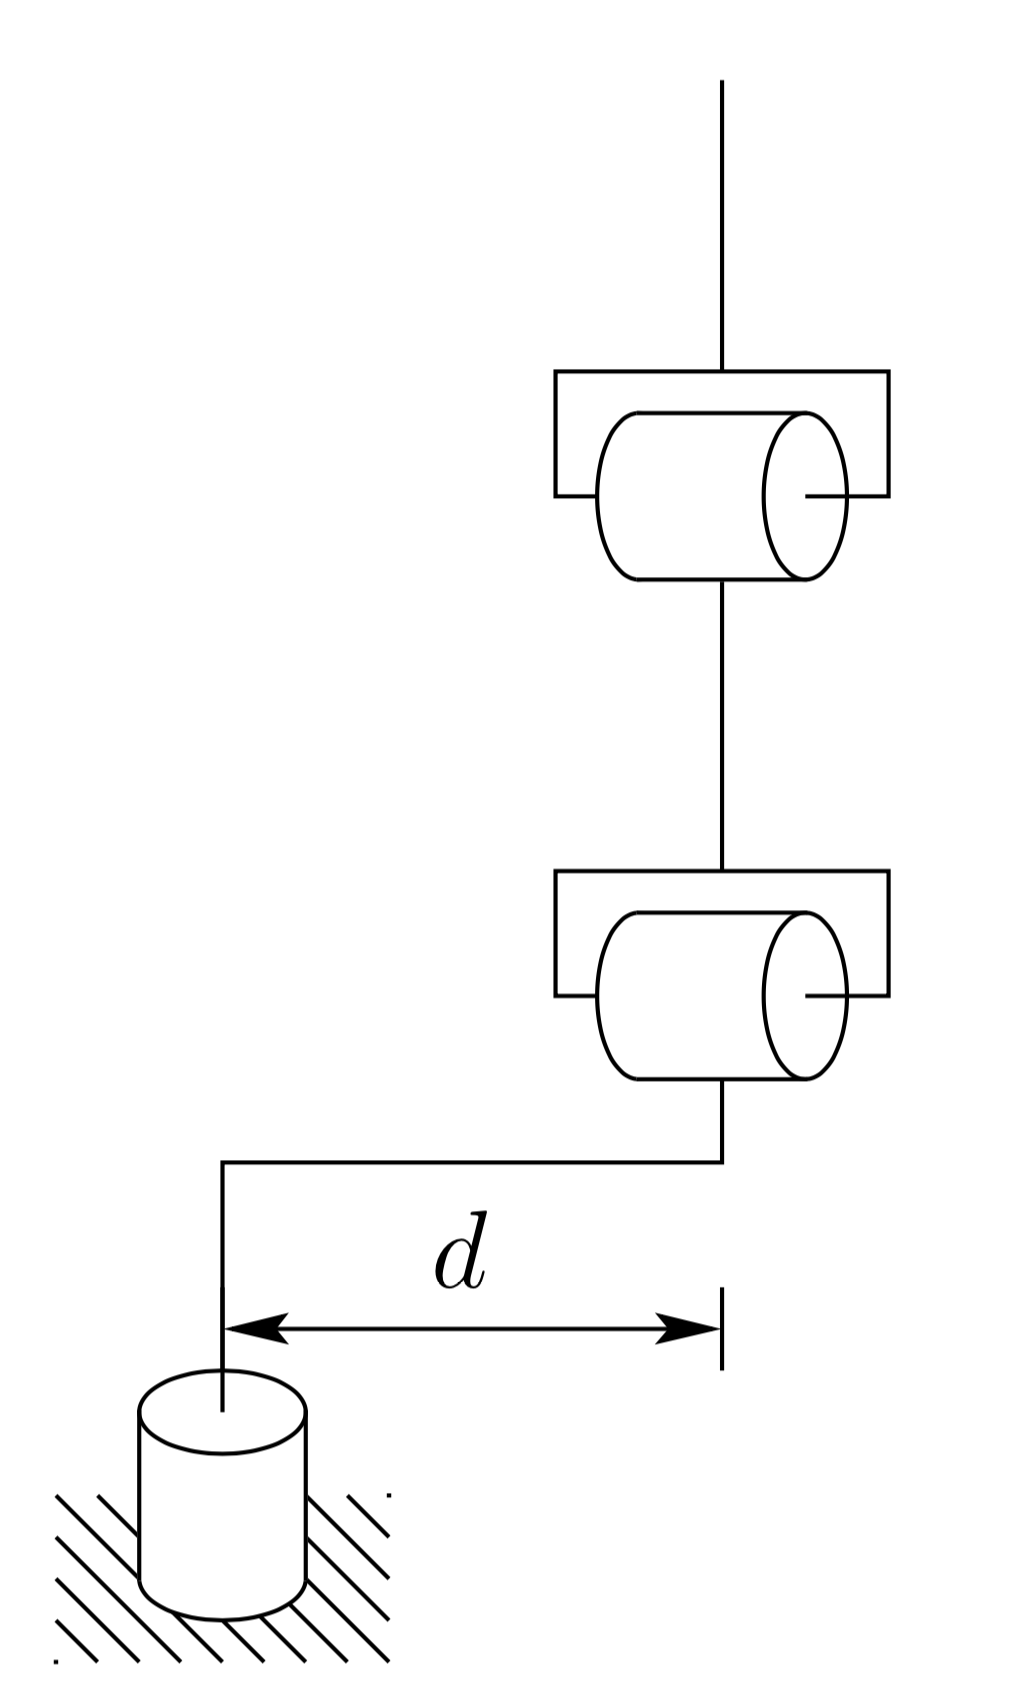
\includegraphics[width=.25\textwidth]{offset}
  \caption[Elbow Manipulator Configuration with Link Offset]{Elbow Manipulator Configuration with Link Offset \cite{robo}}
  \label{fig:offset}
\end{figure}
As shown in \emph{Figure \ref{fig:offset}}, the line directly above the first joint of the manipulator is offset such that the axes of the other joints are unable to become collinear with the base axis; this prevents singularity but causes a void in the detxterous workspace.
\subsubsection{The system end effector shall maintain a positional accuracy magnitude of \(\pm 1\) mm and an orientation accuracy of \(\pm 5^{\circ}\) eigen angle from the base frame.}
To ensure that the robot has educational value, the accuracy must be defined so that any desired positions and movements are achieved with sufficient accuracy.
\begin{enumerate}
  \item \textit{The system shall accommodate a process in which the end user can calibrate the end effector position and orientation to within 0.5 mm and 1 degree of the manipulator’s precision.}
\end{enumerate}
The addition of a calibration process allows the removal of any systematic errors, such as drift. The theoretical limit of the calibration process is the difference between the precision and accuracy metrics of the system.
\subsubsection{The system end effector shall maintain a pose repeatability magnitude between 0.1—1.5 mm for the position and \(\pm 4^{\circ}\) eigen angle from the base frame for the orientation.}
\begin{enumerate}
  \item \textit{Joint one and two of the system shall possess an angle error of no more than .025 degrees.}
\end{enumerate}
Being that joint one and two are the first two rotational elements in the system, their error will propagate the most to the end effector's position.
\begin{enumerate}[resume]
  \item \textit{Joint three of the system shall possess an angle error of no more than .03 degrees.}
\end{enumerate}
Since joint three is closer to the end effector it's error will not propagate as severely throughout the system.
\begin{enumerate}[resume]
  \item \textit{Joints four, five, and six shall possess an angle error of no more than .29 degrees.}
\end{enumerate}
The spherical wrist is the closest to the end effector's final position and therefore has the least error propagation.

\subsubsection{The system’s reachable workspace shall be a hemisphere with a radius of 300-700 mm.}
This workspace will provide enough movement to manipulate objects in order to perform basic tasks.
\begin{enumerate}
  \item \textit{The manipulator shall have a maximum reach between 300 and 700 mm.}
\end{enumerate}
This workspace will provide enough movement to manipulate objects in order to perform basic tasks.
\begin{enumerate}[resume]
  \item \textit{The length of link one, two, three, and the wrist shall be 161.5 mm, 250 mm, 250 mm, and 143 mm respectively.}
\end{enumerate}
\subsubsection{The system’s dexterous workspace shall contain a hemispherical shell within the reachable workspace with a thickness of 280 mm.}\label{sec:zero}
This workspace will provide enough movement to manipulate objects in order to perform basic tasks. 280mm is slightly greater than the length of letter paper.
\begin{enumerate}
  \item \textit{The rotational limit of joint one, two, three, four, five, and six shall be \(\pm180^{\circ}\), \(-9.7^{\circ}\) to \(177.5^{\circ}\), \(-150.6^{\circ}\) to \(-19.3^{\circ}\), \(\pm180^{\circ}\), \(-180^{\circ}\) to \(-1.6^{\circ}\), and \(\pm180^{\circ}\) respectively.}
\end{enumerate}
The angles stated are with respect to the kinematic model shown in \emph{Figure \ref{fig:zero}}. To be fully dexterous within our 280 mm dexterous workspace the manipulator must have the joint angles specified above. The joint limitations were calculated by iteratively verifying the orientation about every point within the quarter hemisphere cross section seen in \emph{Figure \ref{fig:dex2}} (see Appendix, p. \pageref{sec:app}).
  \begin{figure}[htp]
    \centering
    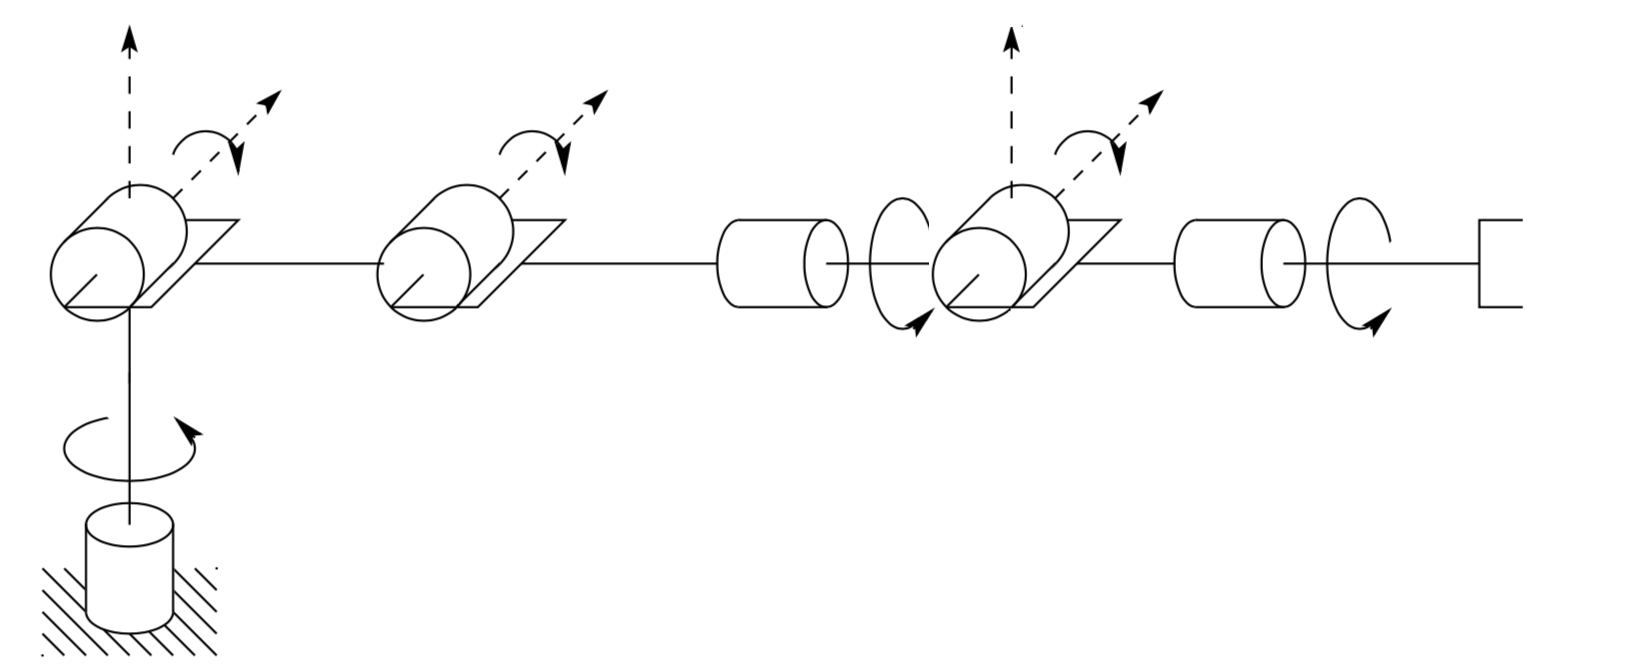
\includegraphics[width=.75\textwidth]{zero}
    \caption[Kinematic Model Representing Zeroed Configuration]{Kinematic Model Representing Zeroed Configuration \cite{robo}}
    \label{fig:zero}
  \end{figure}
\subsubsection{The system shall have a removable end effector capable of picking and placing a low-odor chisel tip Expo dry erase marker.}
This creates a robot capable of performing a variety of basic tasks, which enhances its educational value.
\begin{enumerate}
  \item \textit{The system shall use a parallel gripper that can close to 18mm.}
\end{enumerate}
The diameter of a low-odor chisel tip Expo dry erase marker is approximately 18 mm.
\begin{enumerate}[resume]
  \item \textit{The end effector shall attach to the manipulator using screws configured in a pattern that can accommodate a Dynamixel AX-12A servo.}
\end{enumerate}
It is expected that a majority of end effector styles will have to accommodate for a servo to facilitate actuation, therefore a pattern was chosen to standardize the mounting.


\subsubsection{The system shall be able to write with a low-odor chisel tip Expo dry erase marker.}
\begin{enumerate}
  \item \textit{The end effector shall be able to support 0.004 Newton meter moments about the axes normal to its gripping surfaces.}
\end{enumerate}
  The coefficient of friction between the Expo marker and paper can be approximated and given the weight of an Expo marker the approximate grip strength of the end effector can be calculated.
\hiddensubsection{Software}
The following requirements and specifications are software specific and determine the attributes of the operating system.
\subsubsection{The system shall be open source.}
This will create an easily obtainable, low cost method of distributing the system’s source code, which may be modified for personal use.
\begin{enumerate}
  \item \textit{The software shall be hosted publicly on an online repository and maintain an MIT license for distribution.}
\end{enumerate}
  This allows the end-user to freely download and modify the code without licensing. The MIT license disregards any legal obligation to code upkeep and documentation by the original author.

\subsubsection{The system shall be capable of operating given only desired end effector cartesian coordinates specified with respect to the base frame.}
\begin{enumerate}
  \item \textit{The system shall have a user interface capable of accepting the end-effector’s desired cartesian position and Euler angle orientation as a six element row vector.}
\end{enumerate}
  The system software interface facilitates an untrained user to operate without the advanced knoledge of the system's kinematics.
\begin{enumerate}[resume]
  \item \textit{The system shall be capable of performing floating point arithmetic.}
\end{enumerate}
The solution for the inverse kinematics requires the ability to perform high level arithmetic with little error.

\newpage
\section{Preliminary Design}
The preliminary design section represents the most up-to-date status of the project and also encompasses information pertaining to several different specific design choices that had to be considered. The computer aided design section contains information regarding the physical design of the manipulator as well as noting key design features; the actuator analysis section contains information regarding actuator considerations and calculations being that the servo motors play an essential role in the functionality of the final system.
\subsection{Computer Aided Design}
The manipulator will be six degrees of freedom and will feature a spherical wrist. This design incorporates two different differential drive gearboxes that each control two degrees of freedom. This is to reduce the amount of required torques from the motors on the shoulder joint and reduce size in the wrist. In order to achieve accuracy requirements, timing belts are incorporated into the design in order to control the first three degrees of freedom. The following figure shows the join configuration used in the design of the manipulator.

\begin{figure}[htp]
  \center
  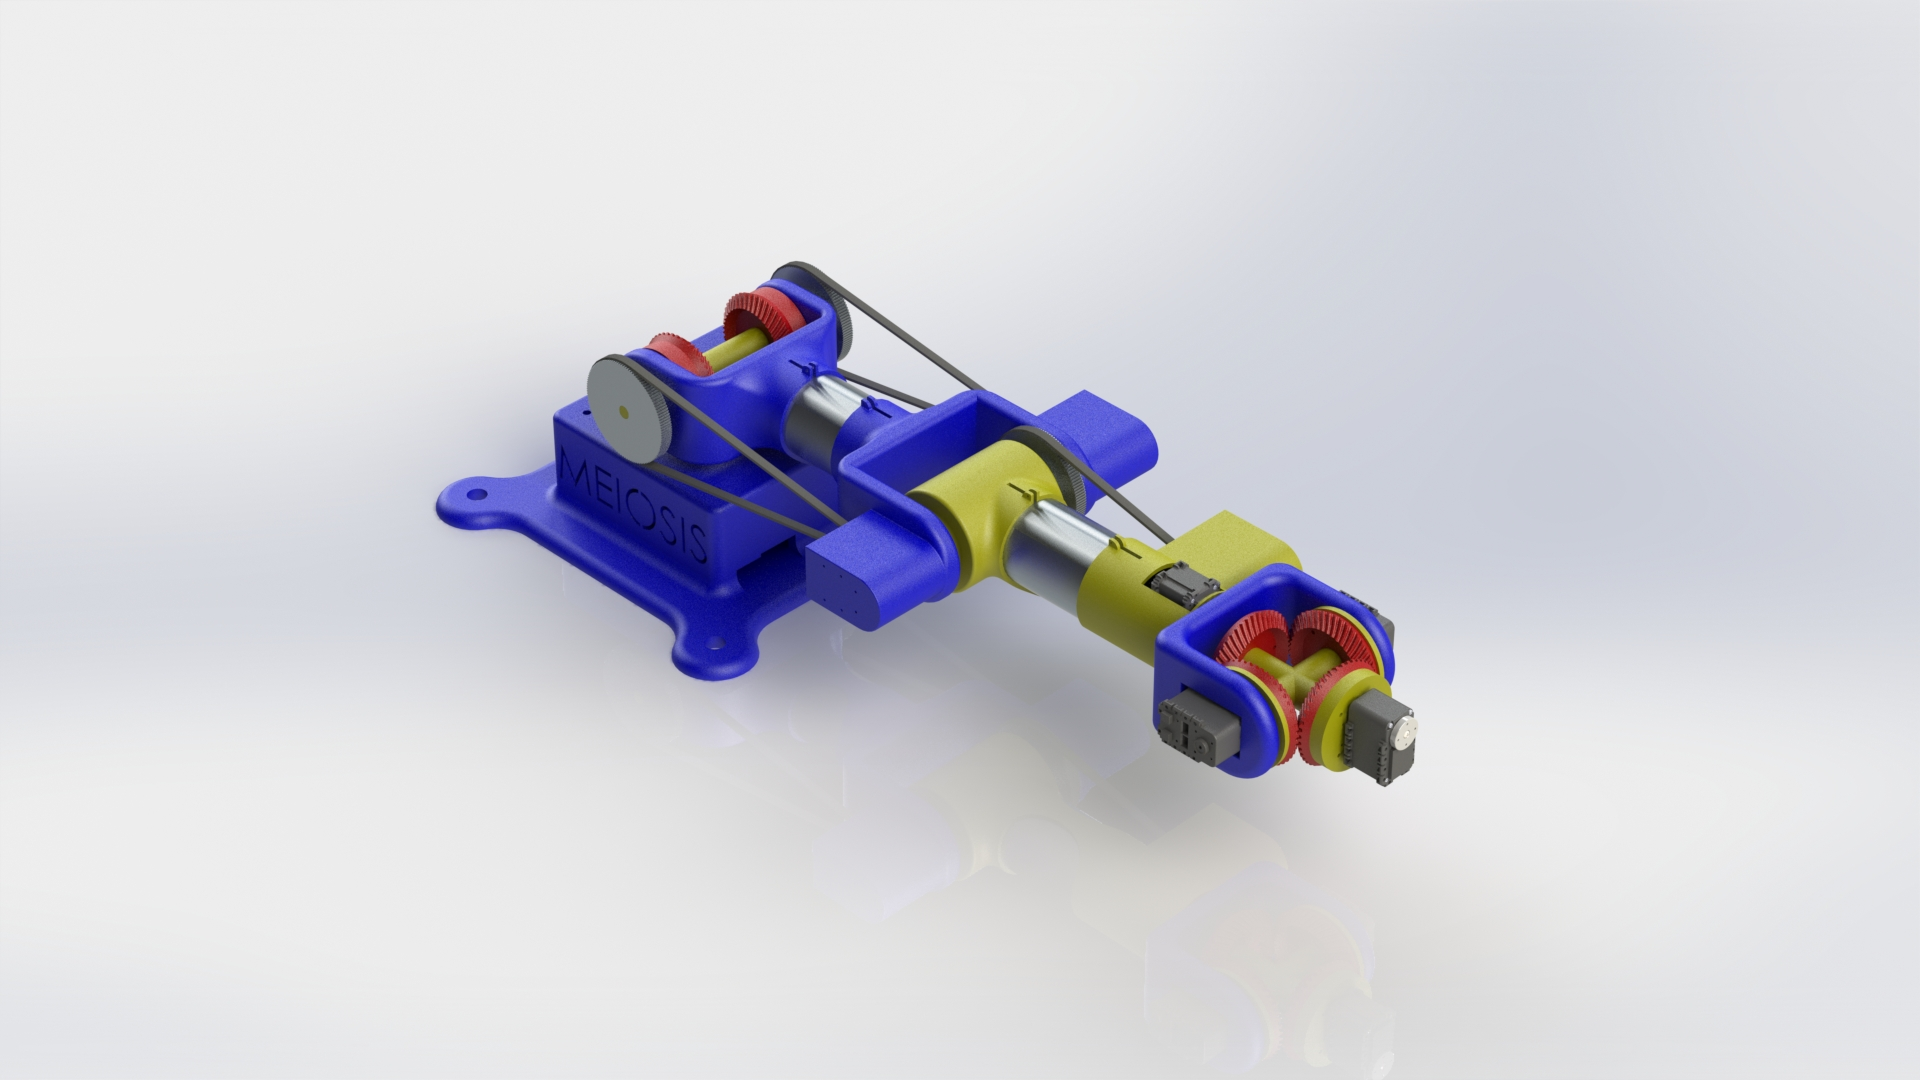
\includegraphics[width=.85\textwidth,frame]{meiosis_zeroed}
  \caption{Manipulator in Zeroed Configuration with Callouts}
  \label{fig:meiosis_zeroed}
\end{figure}
\emph{Figure \ref{fig:meiosis_zeroed}} shows the zeroed configuration for the manipulator with callouts showing the link locations.
\begin{enumerate}[label=\alph*.]
  \item The \emph{Manipulator Base} is designed to hold the Raspberry Pi and power supply. The base features holes for airflow and I/O connections.
  \item \emph{Link 1 \& Differential Drive} have three bevel gears to create the first differential drive rotational joint of the manipulator.
  \item \emph{Link 2} has servos located at the end of the link to control the movement for the first two degrees of freedom at the shoulder and are connected to link 1 using timing belts.
  \item \emph{Link 3} contains two servos attached to the link that control the third degree of freedom (the elbow) and the fourth degree of freedom which is the first degree of freedom for the wrist.
  \item \emph{Link 4 }houses the servos used to control the fifth and sixth degree of freedom, which are both in the wrist’s differential drive gearbox.
  \item \emph{Link 5} provides support for the wrist’s differential drive gearbox.
  \item The \emph{End Effector} features connection points to hold a Dynamixel AX-12A smart servo.
\end{enumerate}
% \emph{Figure \ref{fig:meiosis_zeroed}} shows the zeroed configuration for the manipulator with callouts showing the link locations. Point (a) shows the base of the manipulator. This is designed to hold the Raspberry Pi and power supply. The base features holes for airflow and I/O connections. Point (b) shows the first link of the robot and is the location of the first differential drive gearbox. Point (c) shows the second link of the robot, the servos located at the end of the link control the movement for the first two degrees of freedom at the shoulder and are connected to link 1 using timing belts. Point (d) shows the third link of the robot, there are two servos attached to the link that control the third degree of freedom (the elbow) and the fourth degree of freedom which is the first degree of freedom for the wrist. Point (e) shows the fourth link of the manipulator which houses the servos used to control the fifth and sixth degree of freedom, which are both in the wrist’s differential drive gearbox. Point (f) shows the fifth and final link of the robot. This link is support for the wrist’s differential drive gearbox. Finally, point (g) shows the end effector which features connection points to hold a Dynamixel AX-12A smart servo. The next figure shows key features that are unique to links two and three.

\begin{figure}[htp]
  \center
  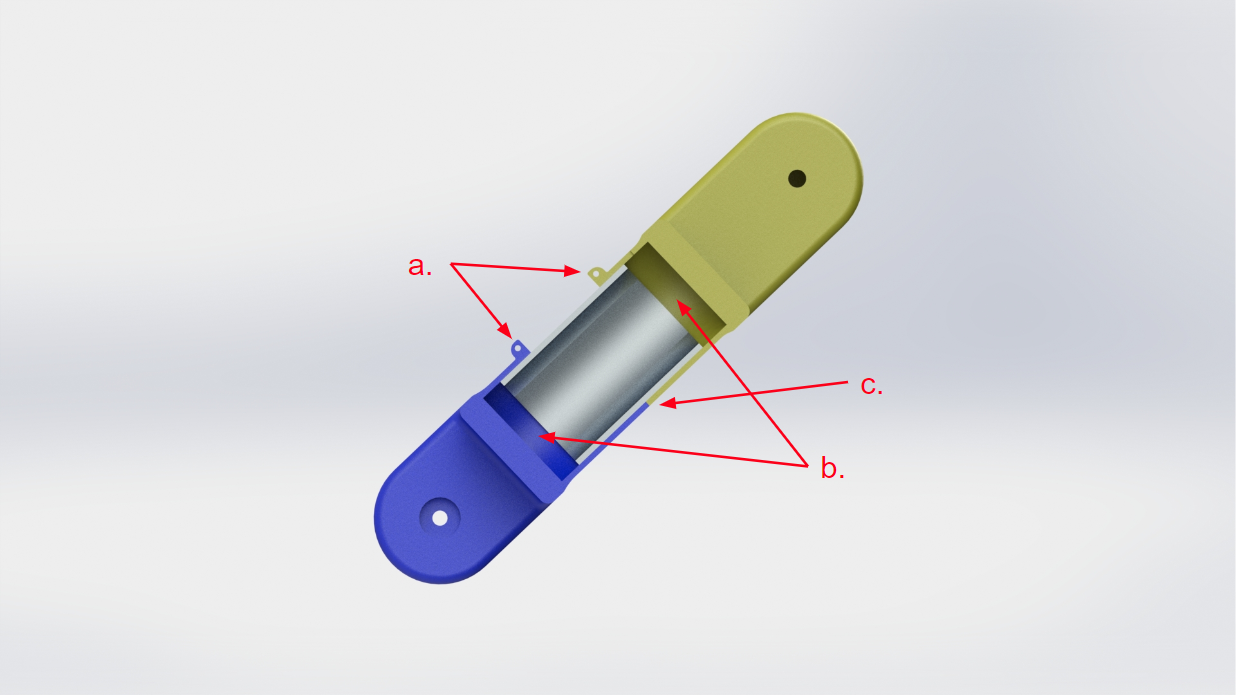
\includegraphics[width=.85\textwidth,frame]{linkx}
  \caption{Link Cross Section}
  \label{fig:linkx}
\end{figure}

\emph{Figure \ref{fig:linkx}} shows the cross-section for link two with callouts for key features in the design.
\begin{enumerate}[label=\alph*.]
  \item \emph{Clamping mechanisms} connect the aluminum pipe to the 3-D printed parts. This will allow for an easy way to assemble the manipulator while allowing for a large amount of tolerance in the length of the pipe when manufacturing the part.
  \item Shows an example of the gaps between the aluminum pipe and the 3-D printed parts.
  \item Shows where the 3-D printed parts will line up to ensure that the link is the correct length and orientation.
\end{enumerate}
% Point (a) shows two clamping mechanisms that will be used to connect the aluminum pipe to the 3-D printed parts. This will allow for an easy way to assemble the manipulator while allowing for a large amount of tolerance in the length of the pipe when manufacturing the part. Point (b) shows an example of the gaps between the aluminum pipe and the 3-D printed parts. Point (c) shows where the 3-D printed parts will line up to ensure that the link is the correct length and orientation.
\emph{Figure \ref{fig:assy_mech}} contains an image of the design utilized to keep the assembly of the robot easy and practical.
\newpage

\begin{figure}[htp]
  \center
  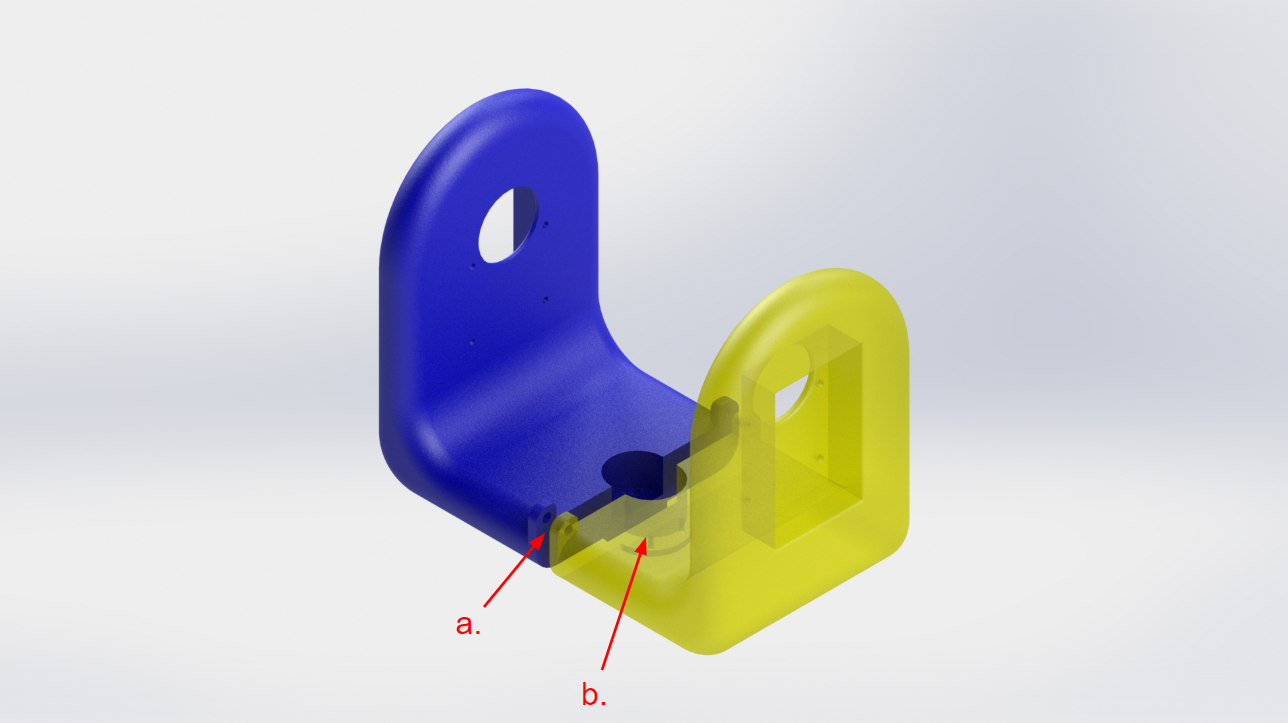
\includegraphics[width=.65\textwidth,frame]{assy_mech}
  \caption{Link 4 Assembly Mechanism}
  \label{fig:assy_mech}
\end{figure}

\emph{Figure \ref{fig:assy_mech}}  shows the link in the wrist that utilizes a special design to ensure proper assembly. The link itself is two parts which connect together on both sides of the link at point (a), this allows for the differential gearbox to be assembled and inserted into the wrist without interference from link 4. Once assembled, the link will attach to the smart servo at point (b).



\subsubsection{Pulleys}
A 12 tooth and 120 tooth pulleys provide a 10:1 gear ratio and use a 0.25 in wide MXL belt. The center distance between the pulleys must be at least 5.43 in to have 5 teeth meshing. Because of the high gear ratio, greater distances do not increase the number of teeth in mesh. \emph{Figure \ref{fig:pulley12}} shows the distance between the manipulator’s first two pulleys is 235.185 mm or 9.259 in, which corresponds to a belt with 300 and pitch diameter of 24 in.
\begin{figure}[htp]
  \center
  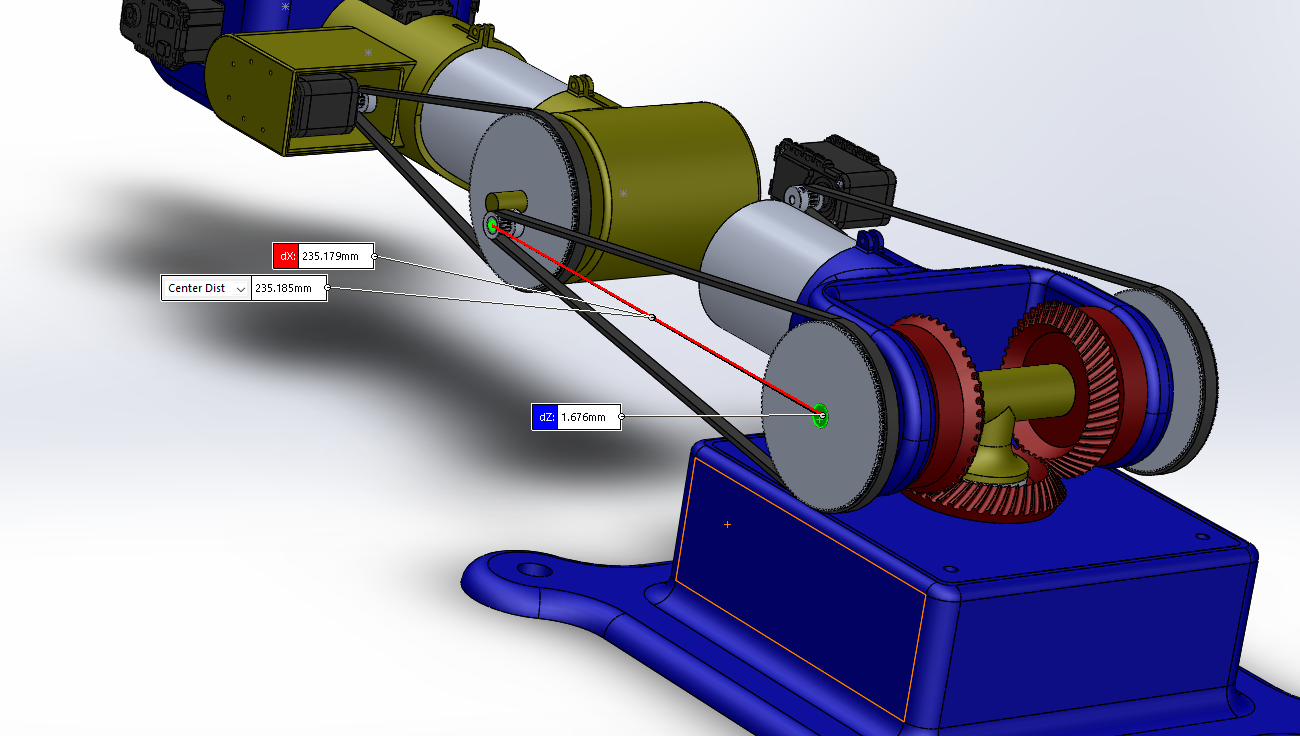
\includegraphics[width=.65\textwidth,frame]{pulley12}
  \caption{Pulley 1-2 Center Distance}
  \label{fig:pulley12}
\end{figure}
\emph{Figure \ref{fig:pulley3}} shows the center distance between the second pulleys is 139.960 mm or 5.510 in. The corresponding belt has 208 teeth with a 16.6 in pitch diameter.
\begin{figure}[htp]
  \center
  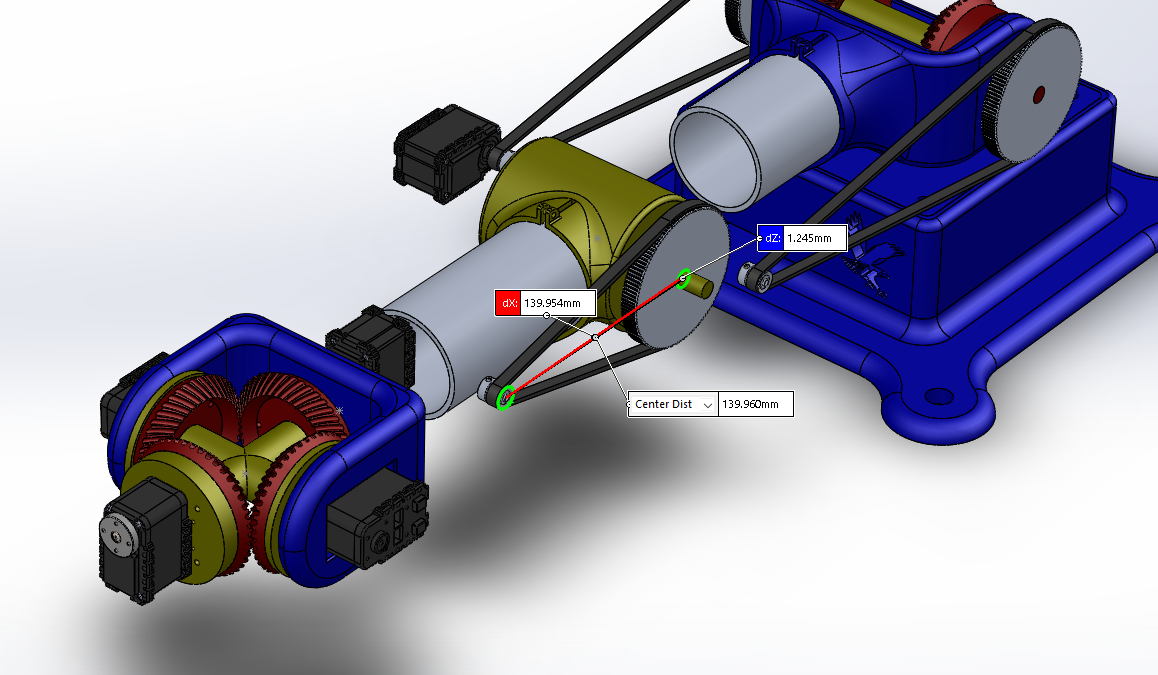
\includegraphics[width=.65\textwidth,frame]{pulley3}
  \caption{Pulley 3 Center Distance}
  \label{fig:pulley3}
\end{figure}
\subsection{Actuator Analysis}
Dynamixel does not provide a stall torque for the MX-12W servo, however it does provide stall torque data for two similar servos. The MX-12W’s stall torque can be found from the stall torque data since the motor are the same. The stall torque of the MX-12W should be comparable to the AX-12W’s stall torque. The MX-12W and AX-12W operate at the same 12 V voltage, 32:1 gear ratio, and 470 rpm no load output speed. The AX-12A also operates at 12 V, but at with a 254:1 gear ratio and 59 rpm no load output speed. Torque and current are inversely related. If the AX-12A’s and AX-12W’s motors are the same, then when operating at the same voltage, the output speed of the AX-12W should equal to the output speed of the AX-12A multiplied by the ratio of the servos’ gear ratios and the torque of the AX-12W should be the AX-12A’s torque multiplied by the inverse of the gear ratios ratio:
\[ 59\cdot\frac{254}{32}=468 \cong 470 \]
The AX-12A’s and MX-12W’s stall torques are 1.5Nm and 0.21Nm, respectively \cite{dyna}:
\[ 1.5\cdot\frac{32}{254}=0.189\cong0.21\text{Nm} \]
Therefore, the AX-12A and MX-12W use the same motor. Additionally, if operating at the same voltage, the stall torque is defined by the no load output speed and gear ratio. Since the MX-12W and AX-12A operate at the same 12 V voltage with the same 32:1 gear ratio and 470 rpm no load output speed, their stall torques should be the same. More specifically, it is between the AX-12W’s and the gear reduced AX-12A’s stall torques of 0.21Nm and 0.189Nm, respectively. Therefore, the stall MX-12W’s stall torque is within 0.01Nm of 0.2Nm. The manipulator is designed for the worst case scenario: 0.19 Nm.

The first differential has its greatest torque when the manipulator is in the zeroed configuration. In the zeroed configuration, the arm is outstretched with gravity acting perpendicular to the arm’s length. Since the manipulator must only support a chisel tip dry erase Expo marker, the maximum torque may be approximated as the manipulator’s arm’s mass acting acting near the centroid. More mass from the servos and longer aluminum support in link 3 place the center of mass closer to the end-effector than the base. Therefore, the point at which the arm’s mass acts is assumed to be 273 mm from the base. These calculations will be further revised with mass parameters from the STL files generating the open and closed loop simulations. \emph{Table \ref{tab:arm1}} estimates the manipulator’s arm’s mass.
\begin{table}[htp]
  \center
  \caption{Manipulator Link 1 Mass Tabulations}
  \label{tab:arm1}
\begin{tabular}{cc|cc}
  \textbf{Item} & \textbf{Specifications} & \textbf{Weight (g)} & \textbf{Notes} \\\hline
  3-D Printed Materials & 30\% infill & 353 & 100\% infill: 1177g \\
  Servos & 7 low torque & 385 & 55 $\sfrac{\text{g}}{\text{servo}}$ \\
  Aluminum Support & .75$''$  OD .125$''$  thick 1$'$ long & 287 & 44.23 $\sfrac{\text{g}}{\text{in}}^3$ \\
  Bearings & 5 bearings & 60 & 12 $\sfrac{\text{g}}{\text{bearing}}$ \\
  End Effector & & 50 & Approx. \\
  Safety Factor & & 205 & \\
  & \textbf{Total} & 1340 & \\
\end{tabular}
\end{table}

The total mass of 1340g as seen in \emph{Table \ref{tab:arm1}} yields a moment of 0.361 Nm or 3.685 kgm. To generate smooth motions, Dynamixel recommends operating at one fifth of the stall torque. Therefore, the actual maximum required torque is 1.805 Nm. An MX-12W provides 0.19 Nm of torque, necessitating a 10:1 gear ratio. While the AX-12A provides a greater torque of 1.5 Nm, it would also require gearing. It is only precise to 0.8 degrees, while the specifications require at least 0.29 degrees of precision for joints one and two. Further, the AX-12A only receives position feedback for 300 degrees of its rotation and cannot track multiple rotations, making it untenable for the base motor, which must rotate more than 360 degrees.

The third joint’s torque requirements can be approximated in the same manner. However, links three, four, and five’s masses are assumed to act 200 mm from the third joint 3. \emph{Table \ref{tab:arm2}} estimates the links’ masses.

\begin{table}[htp]
  \center
  \caption{Manipulator Link 2 Mass Tabulations}
  \label{tab:arm2}
\begin{tabular}{cc|cc}
\textbf{Item} & \textbf{Specifications} & \textbf{Weight (g)} & \textbf{Notes} \\\hline
3-D Printed Materials & 30\% infill & 180 & 100\% infill: 1177g \\
Servos & 4 low torque & 220 & 55 $\sfrac{\text{g}}{\text{servo}}$ \\
Aluminum Support & .75$''$ OD .125$''$ thick 1$'$ long & 140 & 44.23 $\sfrac{\text{g}}{\text{in}}^3$ \\
Bearings & 5 bearings & 36 & 12 $\sfrac{\text{g}}{\text{bearing}}$ \\
End Effector & & 50 & Approx. \\
Safety & & 205 & \\
& \textbf{Total} & 831 & \\
\end{tabular}
\end{table}

The resulting moment is 1.630 Nm, which can be satisfied by the same motor and gear ratio used on the base.

\subsection{Forward Kinematics}
The forward kinematics of the manipulator are described by the equations below, where the reference coordinate frames are given by \emph{Figure \ref{fig:coords}}.
\begin{figure}[htp]
  \centering
  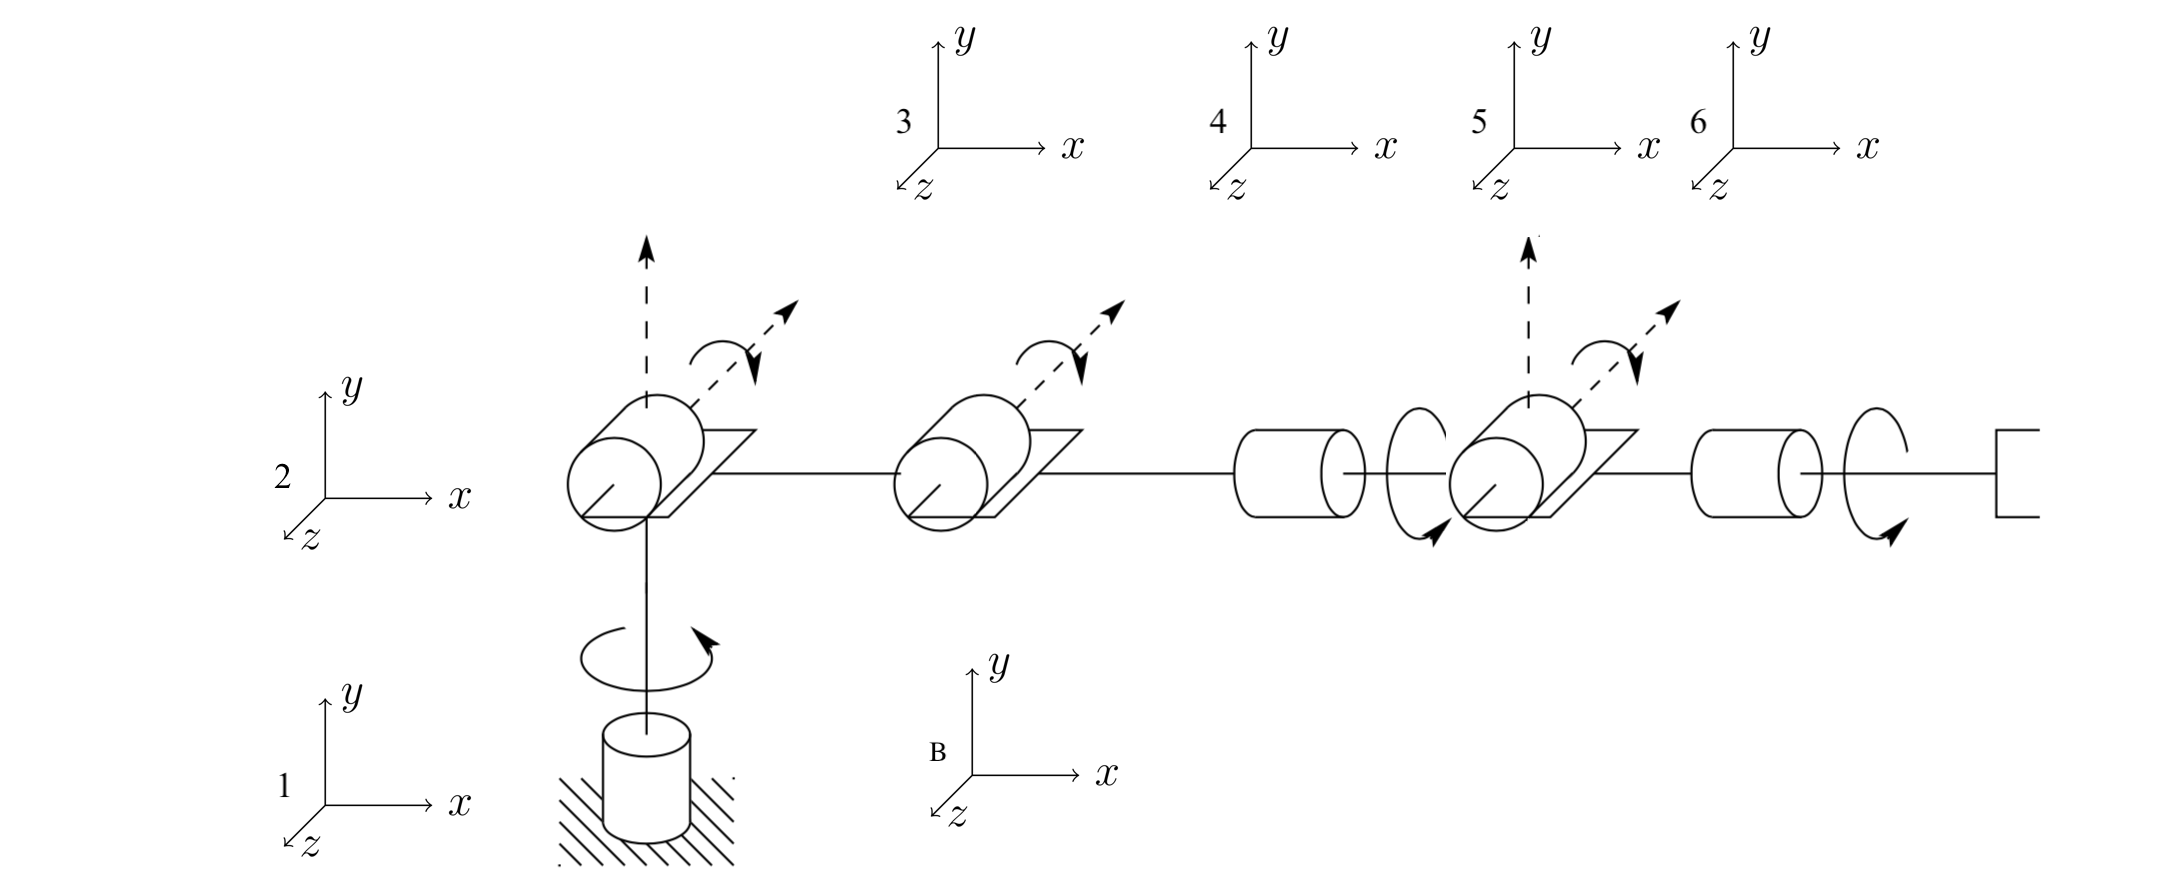
\includegraphics[width=.9\textwidth]{zero2}
  \caption{Coordinate Systems}
  \label{fig:coords}
\end{figure}

Given the lengths of each of the manipulator links,
\[
\begin{aligned}
  ^I_Br_1 = \begin{bmatrix} 0\\0\\ \ell_b\end{bmatrix} & \quad
  ^1_1r_2 = \begin{bmatrix} 0\\0\\ \ell_1\end{bmatrix} & \quad
  ^2_2r_3 = \begin{bmatrix} 0\\\ell_2\\ 0\end{bmatrix} & \quad
  ^3_3r_4 = \begin{bmatrix} 0\\\ell_3\\ 0\end{bmatrix} & \quad
  ^4_4r_5 = \begin{bmatrix} 0\\\ell_4\\ 0\end{bmatrix} & \quad
  ^5_5r_6 = \begin{bmatrix} 0\\\ell_5\\ 0\end{bmatrix} & \quad
\end{aligned}
\]
The position of each link relative to the inertial frame is given as:
\[
\begin{aligned}
^I_Br_1 &= {}_Br_1 &\quad
^I_Br_2 &= r_1 + {}^IT_1 {}^1_1r_2 &\quad
^I_Br_3 &= r_2 + {}^IT_2 {}^2_2r_3 \\
^I_Br_4 &= r_3 + {}^IT_3 {}^3_3r_4 &\quad
^I_Br_5 &= r_4 + {}^IT_4 {}^4_4r_5 &\quad
^I_Br_6 &= r_5 + {}^IT_5 {}^5_5r_6
\end{aligned}
\]

\[
\begin{aligned}
  ^I_Br_1 =&
  \begin{bmatrix}
    0\\ 0\\ \ell_b
  \end{bmatrix} & \quad
  ^I_Br_2 =
  \begin{bmatrix}
    0\\ 0\\ \ell_b + \ell_1
  \end{bmatrix} & \quad
  ^I_Br_3 =
  \begin{bmatrix}
    -\ell_2c_{\theta_2}s_{\theta_1}\\
    \ell_2c_{\theta_{12}}\\
    \ell_b+\ell_1+\ell_2s_{\theta_2}
  \end{bmatrix} & \quad
  ^I_Br_4 =
  \begin{bmatrix}
    -s_{\theta_1}(\ell_3c_{\theta_{23}} + \ell_2c_{\theta_2}) \\
    c_{\theta_1}(\ell_3c_{\theta_{23}} + \ell_2c_{\theta_2}) \\
    \ell_1 + \ell_b + \ell_3s_{\theta_{23}} + \ell_2s_{\theta_2}
  \end{bmatrix} \\
\end{aligned}
  \]
  \[
  ^I_Br_5 =
  \begin{bmatrix}
    -s_{\theta_1}(\ell_3c_{\theta_{23}} + \ell_4c_{\theta_{23}} + \ell_2c_{\theta_2}) \\
    c_{\theta_1}(\ell_3c_{\theta_{23}} + \ell_4c_{\theta_{23}} + \ell_2c_{\theta_2}) \\
    \ell_1 + \ell_b + \ell_3s_{\theta_{23}} + \ell_4s_{\theta_{23}} + \ell_2s_{\theta_2}
  \end{bmatrix}
  \]
  \[
  ^I_Br_6 =
  \begin{bmatrix}
  \begin{aligned}
      &\ell_5c_{\theta_1}s_{\theta_4}s_{\theta_5} - \ell_4c_{\theta_{23}}s_{\theta_1} - \ell_2c_{\theta_2}s_{\theta_1} - \ell_5c_{\theta_{23}}c_{\theta_5}s_{\theta_1} - \ell_3c_{\theta_{23}}s_{\theta_1} \\
      &\qquad\qquad+ \ell_5c_{\theta_2}c_{\theta_4}s_{\theta_1}s_{\theta_3}s_{\theta_5} + \ell_5c_{\theta_3}c_{\theta_4}s_{\theta_1}s_{\theta_2}s_{\theta_5} \\
      &\ell_5(s_{\theta_5}(s_{\theta_1}s_{\theta_4} - c_{\theta_4}(c_{\theta_1}c_{\theta_2}s_{\theta_3} + c_{\theta_1}c_{\theta_3}s_{\theta_2})) - c_{\theta_5}(c_{\theta_1}s_{\theta_2}s_{\theta_3} - c_{\theta_1}c_{\theta_2}c_{\theta_3})) \\
      &\qquad\qquad -\ell_3(c_{\theta_1}s_{\theta_2}s_{\theta_3} - c_{\theta_1}c_{\theta_2}c_{\theta_3}) -\ell_4(c_{\theta_1}s_{\theta_2}s_{\theta_3} - c_{\theta_1}c_{\theta_2}c_{\theta_3}) + \ell_2c_{\theta_1}c_{\theta_2} \\
      &\ell_1 + \ell_b + \ell_3s_{\theta_{23}} + \ell_4s_{\theta_{23}} + \ell_2s_{\theta_2} + \dfrac{\ell_5c_{\theta_{23}}s_{\theta_{45}}}{2} + \ell_5s_{\theta_{23}}c_{\theta_5} - \dfrac{\ell_5s_{\theta_4 - \theta_5}c_{\theta_{23}}}{2}
    \end{aligned}
  \end{bmatrix}
\]
\newpage
Given the direction cosine matrices,

\[
rotx(\theta) = \begin{bmatrix}
 1 & 0 & 0\\
 0 & \cos(\theta) & -\sin(\theta) \\
 0 & \sin(\theta) & \cos(\theta)
\end{bmatrix}~,\quad
roty(\theta) = \begin{bmatrix}
 1 & 0 & 0\\
 0 & \cos(\theta) & -\sin(\theta) \\
 0 & \sin(\theta) & \cos(\theta)
\end{bmatrix}
\]
\[
rotz(\theta) = \begin{bmatrix}
 \cos(\theta) & 0 & \sin(\theta)\\
  0 & 1 & 0 \\
 -\sin(\theta) & \cos(\theta) & 0
\end{bmatrix}
\]
The orientation of each link with respect to the inertial frame is given as:
\[
\begin{aligned}
^IT_1 &= rotz(\theta_1) \\
^IT_2 &= rotz(\theta_1)~rotx(\theta_2)\\
^IT_3 &= rotz(\theta_1)~rotx(\theta_2)~rotx(\theta_3)\\
^IT_4 &= rotz(\theta_1)~rotx(\theta_2)~rotx(\theta_3)~roty(\theta_4)\\
^IT_5 &= rotz(\theta_1)~rotx(\theta_2)~rotx(\theta_3)~roty(\theta_4)~rotx(\theta_5)\\
^IT_6 &= rotz(\theta_1)~rotx(\theta_2)~rotx(\theta_3)~roty(\theta_4)~rotx(\theta_5)~roty(\theta_6)\\
\end{aligned}
\]
\[
\begin{aligned}
  ^IT_1 =
  \begin{bmatrix}
    c_{\theta_1}& -s_{\theta_1}& 0\\
    s_{\theta_1}&  c_{\theta_1}& 0\\
    0&            0& 1\\
  \end{bmatrix} & \quad
  ^IT_2 =
  \begin{bmatrix}
    c_{\theta_1}& -c_{\theta_2}s_{\theta_1}&  s_{\theta_1}s_{\theta_2}\\
    s_{\theta_1}&  c_{\theta_1}c_{\theta_2}& -c_{\theta_1}s_{\theta_2}\\
    0&              s_{\theta_2}&              c_{\theta_2}\\
  \end{bmatrix} & \quad
  ^IT_3 =
  \begin{bmatrix}
    c_{\theta_1}& -c_{\theta_{23}}s_{\theta_1}&  s_{\theta_{23}}s_{\theta_1}\\
    s_{\theta_1}&  c_{\theta_{23}}c_{\theta_1}& -s_{\theta_{23}}c_{\theta_1}\\
    0&              s_{\theta_{23}}&              c_{\theta_{23}}\\
  \end{bmatrix}
\end{aligned}
\]
\[
^IT_4 =
\begin{bmatrix}
c_{\theta_1}c_{\theta_4} - s_{\theta_{23}}s_{\theta_1}s_{\theta_4}& -c_{\theta_{23}}s_{\theta_1}& c_{\theta_1}s_{\theta_4} + s_{\theta_{23}}c_{\theta_4}s_{\theta_1}\\
c_{\theta_4}s_{\theta_1} + s_{\theta_{23}}c_{\theta_1}s_{\theta_4}&  c_{\theta_{23}}c_{\theta_1}& s_{\theta_1}s_{\theta_4} - s_{\theta_{23}}c_{\theta_1}c_{\theta_4}\\
-c_{\theta_{23}}s_{\theta_4}&              s_{\theta_{23}}&                                       c_{\theta_{23}}c_{\theta_4}\\
\end{bmatrix}
\]
\[
^IT_5 =
\begin{bmatrix}
c_{\theta_1}c_{\theta_4} - s_{\theta_{23}}s_{\theta_1}s_{\theta_4}& s_{\theta_5}(c_{\theta_1}s_{\theta_4} + s_{\theta_{23}}c_{\theta_4}s_{\theta_1}) - c_{\theta_{23}}c_{\theta_5}s_{\theta_1}& c_{\theta_5}(c_{\theta_1}s_{\theta_4} +
 s_{\theta_{23}}c_{\theta_4}s_{\theta_1}) + c_{\theta_{23}}s_{\theta_1}s_{\theta_5}\\
c_{\theta_4}s_{\theta_1} + s_{\theta_{23}}c_{\theta_1}s_{\theta_4}& s_{\theta_5}(s_{\theta_1}s_{\theta_4} - s_{\theta_{23}}c_{\theta_1}c_{\theta_4}) + c_{\theta_{23}}c_{\theta_1}c_{\theta_5}& c_{\theta_5}(s_{\theta_1}s_{\theta_4} - s_{\theta_{23}}c_{\theta_1}c_{\theta_4}) - c_{\theta_{23}}c_{\theta_1}s_{\theta_5}\\
-c_{\theta_{23}}s_{\theta_4}&                                                     s_{\theta_{23}}c_{\theta_5} + c_{\theta_{23}}c_{\theta_4}s_{\theta_5}&                                                     c_{\theta_{23}}c_{\theta_4}c_{\theta_5} - s_{\theta_{23}}s_{\theta_5}\\
\end{bmatrix}
\]
\[
^IT_6 =
\begin{bmatrix}
  ^IT_{6(1,1)} & ^IT_{6(1,2)} & ^IT_{6(1,3)}\\
  ^IT_{6(2,1)} & ^IT_{6(2,2)} & ^IT_{6(2,3)}\\
  ^IT_{6(3,1)} & ^IT_{6(3,2)} & ^IT_{6(3,3)}\\
\end{bmatrix}
\]
\[
\begin{aligned}
^IT_{6(1,1)} &=
c_{\theta_6}(c_{\theta_1}c_{\theta_4} - s_{\theta_{23}}s_{\theta_1}s_{\theta_4}) - s_{\theta_6}(c_{\theta_5}(c_{\theta_1}s_{\theta_4} + s_{\theta_{23}}c_{\theta_4}s_{\theta_1}) + c_{\theta_{23}}s_{\theta_1}s_{\theta_5})\\
^IT_{6(1,2)} &=
s_{\theta_5}(c_{\theta_1}s_{\theta_4} + s_{\theta_{23}}c_{\theta_4}s_{\theta_1}) - c_{\theta_{23}}c_{\theta_5}s_{\theta_1}\\
^IT_{6(1,3)} &=
c_{\theta_6}(c_{\theta_5}(c_{\theta_1}s_{\theta_4} + s_{\theta_{23}}c_{\theta_4}s_{\theta_1}) + c_{\theta_{23}}s_{\theta_1}s_{\theta_5}) + s_{\theta_6}(c_{\theta_1}c_{\theta_4} - s_{\theta_{23}}s_{\theta_1}s_{\theta_4})\\
^IT_{6(2,1)} &=
c_{\theta_6}(c_{\theta_4}s_{\theta_1} + s_{\theta_{23}}c_{\theta_1}s_{\theta_4}) - s_{\theta_6}(c_{\theta_5}(s_{\theta_1}s_{\theta_4} - s_{\theta_{23}}c_{\theta_1}c_{\theta_4}) - c_{\theta_{23}}c_{\theta_1}s_{\theta_5})\\
^IT_{6(2,2)} &=
s_{\theta_5}(s_{\theta_1}s_{\theta_4} - s_{\theta_{23}}c_{\theta_1}c_{\theta_4}) + c_{\theta_{23}}c_{\theta_1}c_{\theta_5}\\
^IT_{6(2,3)} &=
s_{\theta_6}(c_{\theta_4}s_{\theta_1} + s_{\theta_{23}}c_{\theta_1}s_{\theta_4}) + c_{\theta_6}(c_{\theta_5}(s_{\theta_1}s_{\theta_4} - s_{\theta_{23}}c_{\theta_1}c_{\theta_4}) - c_{\theta_{23}}c_{\theta_1}s_{\theta_5})\\
^IT_{6(3,1)} &=
s_{\theta_6}(s_{\theta_{23}}s_{\theta_5} - c_{\theta_{23}}c_{\theta_4}c_{\theta_5}) - c_{\theta_{23}}c_{\theta_6}s_{\theta_4}\\
^IT_{6(3,2)} &=
s_{\theta_{23}}c_{\theta_5} + c_{\theta_{23}}c_{\theta_4}s_{\theta_5}\\
^IT_{6(3,3)} &=
c_{\theta_6}(s_{\theta_{23}}s_{\theta_5} - c_{\theta_{23}}c_{\theta_4}c_{\theta_5}) - c_{\theta_{23}}s_{\theta_4}s_{\theta_6}
\end{aligned}
\]

\subsection{Velocity Kinematics}
The translational and rotational velocties ($\dot{r}$ \& $\omega$) can be found given the geometric jacobian of the body and transformation matrix corresponding to it.
\[
\begin{bmatrix}
  ^B_B\omega_I\\
  ^I_B\dot{r}_B
\end{bmatrix}
= J_B =
\begin{bmatrix}
  ^IT_B(:,3)^T \cdot \dfrac{\partial}{\partial\gamma}{}^IT_B(:,2) \\
  ^IT_B(:,1)^T \cdot \dfrac{\partial}{\partial\gamma}{}^IT_B(:,3) \\
  ^IT_B(:,2)^T \cdot \dfrac{\partial}{\partial\gamma}{}^IT_B(:,1) \\
\end{bmatrix}
\]

\subsection{Inverse Kinematics}
The inverse kinematics can be calculated given desired position and orientation vectors, $o$ and $R$, respecitvely.
\[
\begin{bmatrix}x_c & y_c & z_c \end{bmatrix} = o~,\quad
  R =
  \begin{bmatrix}
    r_{11} & r_{12} & r_{13} \\
    r_{21} & r_{22} & r_{23} \\
    r_{31} & r_{32} & r_{33}
  \end{bmatrix}
\]
\begin{equation}
\begin{aligned}
\text{Inverse Position:}\qquad\qquad&\\
\theta_{1}&= \text{atan2} \left(x_{c},~ y_{c}\right) - \sfrac{\pi}{2}\\
\theta_{2}&= \text{atan2} \left(z_c - \ell_1, ~\sqrt{x_c^2 + y_c^2}\right) - \text{atan2}\left(\ell_3s_3,~\ell_2 + \ell_3c_3\right) \\
\theta_{3}&= \text{atan2} (-\sqrt{1-D^{2}},~ D) \\
& \quad \text { where } D\equiv\frac{x_{c}^{2}+y_{c}^{2}+\left(z_{c}-\ell_{1}\right)^{2}-\ell_{2}^{2}-\ell_{3}^{2}}{2 \ell_{2} \ell_{3}} \\
\text{Inverse Orientation}:\qquad\qquad&\\
^IT_3 &= rotz(\theta_1)~rotx(\theta_2)~rotx(\theta_3) \\
{}^3T_6 &= {}^IT_3^TR \\ % TODO: reference the FK orientation sec#/p.
\theta_4 &= \text{atan2} \left({}^3T_{6(1,2)},~{}^3T_{6(3,2)}\right) \\
\theta_5 &= \text{atan2} \left({{}^3T_{6(3,2)}} / {c_4},~{}^3T_{6(2,2)}\right) \\
\theta_6 &= \text{atan2} \left({}^3T_{6(2,1)},~ -{}^3T_{6(2,3)}\right) \\
\end{aligned}
\nonumber
\end{equation}
% \newpage

\subsection{Equations of Motion}
Given robot dynamics described by \(H(\gamma) \ddot{\gamma}+d(\gamma, \dot{\gamma})+G(\gamma)=F_{\gamma},\) the equations of motion for
the manipulator can be determined. Solving this equation for the acceleration, \(\ddot{\gamma}\), gives:
\begin{equation}
  \ddot{\gamma}=H(\gamma)^{-1}\left(F_{\gamma}-d(\gamma, \dot{\gamma})-G(\gamma)\right)
  \label{eq:eoms}
\end{equation}
Where $H$ is the system mass matrix, $F_{\gamma}$ is the vector of generalized forces, $d$ is the vector of centripital and coriolis effects, and $G$ is gravitational effects.
\[
  \renewcommand{\arraystretch}{1.5}
  H(\gamma) = \sum_B^N J_B(\gamma)^T
  \begin{bmatrix}
    ^B_BJ & \mathring{S}(^B_B\Gamma) ^IT_B^T\\
    ^IT_B\mathring{S}(^B_B\Gamma)^T & m_BI
  \end{bmatrix}
  J_B(\gamma)~,\quad
  ^B_B\Gamma = ^B_Br_{cm}m_b~,\quad \mathring{S}(\omega)r=(\omega\times r)
\]
\[
  \renewcommand{\arraystretch}{1.5}
  d(\gamma,\dot{\gamma}) = \sum_B^N J_B(\gamma)^T
  \begin{bmatrix}
    ^B_BJ & \mathring{S}(^B_B\Gamma) ^IT_B^T\\
    ^IT_B\mathring{S}(^B_B\Gamma)^T & m_BI
  \end{bmatrix}
  \dot{J}_B(\gamma,\dot{\gamma})\dot{\gamma}+J_B(\gamma)^T
  \begin{bmatrix}
    ^B_B\omega_I \times ^B_BJ ^B_B\omega_I \\
    ^IT_B\left(^B_B\omega_I\times(^B_B\omega_I\times^B_B\Gamma)\right)
  \end{bmatrix}
\]
\[
G(\gamma) = \left(\frac{\partial U(^Ir(\gamma))}{\partial\gamma}\right)^T~,\quad U_B = \begin{bmatrix} 0 & 0 & g\end{bmatrix}\left(^I_Br_Bm_B + ^IT_B{}_B^B\Gamma\right)
\]
Where $J_B$ is the jacobian of the body, $\Gamma$ is the vector of first mass moments, $m_B$ is the mass of the body, and $^B_B\omega_I$ is the rotational velocity of the body relative to the inertial frame.
\subsubsection{Actuator Dynamics}
Given robot dynamics described by \(H(\gamma)\ddot{\gamma} + n(\gamma,\dot{\gamma}) = \tau\), the torque, $\tau$, provided by the servo motors is necessary to solve the closed loop dynamics of the system. Assuming the servo is driven by a D.C. motor with proportional derivative control,
\begin{equation}
  \tau_a = Ki_a = J_a\ddot{\theta}_a + b_a\dot{\theta}_a + \tau_L
  \label{eq:motor}
\end{equation}
Where $\tau_a$ is the actuator torque, $K$ is the back-EMF constant, $i_a$ is the motor current, $J_a$ is the armature inertia, $\theta_a,~\dot{\theta}_a,\ddot{\theta}_a$ is the motor position and it's first and second time derivatives respectively, $b_a$ is the viscous friction coefficient, and $\tau_L$ is the torque available for the actuator to do work. The basic equation for a motor is known to be:
\begin{equation}
  V_a = i_aR_a + K\dot{\theta}_a
  \label{eq:va}
\end{equation}
Where $V_a$ is the voltage applied to the actuator and $R_a$ is the armature resistance. Given a gearbox with $\sfrac{\text{in}}{\text{out}}$ ratio $N$ and efficiency $\eta$,
\begin{center}
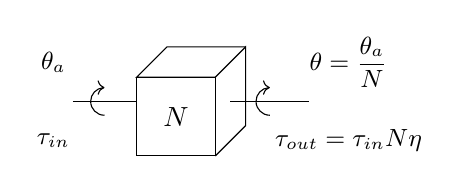
\begin{tikzpicture}
\pgfmathsetmacro{\cubex}{1}
\pgfmathsetmacro{\cubey}{1}
\pgfmathsetmacro{\cubez}{1}
\draw (0,0,0) -- ++(-\cubex,0,0) -- ++(0,-\cubey,0) -- ++(\cubex,0,0) -- cycle;
\draw (0,0,0) -- ++(0,0,-\cubez) -- ++(0,-\cubey,0) -- ++(0,0,\cubez);
\draw (0,0,0) -- ++(-\cubex,0,0) -- ++(0,0,-\cubez) -- ++(\cubex,0,0);
\draw (-2,-.5,-.5) -- ++(.8,0,0) node(a)[midway,above]{} node(b)[midway]{} node(c)[midway,below]{};
\pic [draw,angle radius=5,<-] {angle = a--b--c};
\node at (-2.25,0,-.5) {\small $\theta_a$};
\node at (-2.25,-1,-.5) {\small $\tau_{in}$};
\draw (0,-.5,-.5) -- ++(1,0,0);
\draw (0,-.5,-.5) -- ++(1,0,0) node(a1)[midway,above]{} node(b1)[midway]{} node(c1)[midway,below]{};
\pic [draw,angle radius=5,<-] {angle = a1--b1--c1};
\node at (1.5,0,-.5) {\small $\theta=\dfrac{\theta_a}{N}$};
\node at (1.5,-1,-.5) {\small $\tau_{out}=\tau_{in}N\eta$};
\node at (-.5,-.5,0) {$N$};
\end{tikzpicture}
\end{center}

The motor equation (\ref{eq:motor}) can be expressed in the output coordinates:
\[
Ki_a = J_aN\ddot{\theta} + b_aN\dot{\theta} + \frac{\tau}{N\eta}
\]
Substituing into equation (\ref{eq:va}) and solving for $i_a$:
\[
  i_a = \frac{J_aN}{K}\ddot{\theta} + b_aN\dot{\theta} + \frac{\tau}{N\eta}
\]
\begin{equation}
  V_a = \frac{R_aJ_aN}{K}\ddot{\theta} + \frac{R_ab_aN}{K}\dot{\theta} + \frac{R_a}{KN\eta}\tau + KN\dot{\theta}
  \label{eq:newva}
\end{equation}
Assuming PD control, \(V_a = K_p(\theta-\theta_d) + K_d\dot{\theta}\), where $\theta_d$ is the desired orientation of the actuator, the following solution is found by setting the PD solution equal to (\ref{eq:newva}). After collecting like terms:

\begin{equation}
  \frac{R_aJ_aN}{K}\ddot{\theta} + \left( \frac{R_aJ_aN}{K} - K_d + KN \right)\dot{\theta} - K_p\theta = -K_p\theta_d - \frac{R_a}{KN\eta}\tau
  \label{eq:end1}
\end{equation}
\newpage
The following parameters of the system can be obtained by applying a step input to the system with $\tau=0$ and measuring the characteristics of it's response. Denoting $\zeta$ as the damping ratio and $\omega_n$ as the natural frequency of the system,
\[
  \text{\% Overshoot} = \left( \frac{\theta_{max} - \theta_{ss}}{\theta_{ss}} \right) \times 100~,\quad \zeta = \frac{-\ln(\sfrac{\%\text{OS}}{100})}{\sqrt{\pi^2 + \ln^2(\sfrac{\%\text{OS}}{100})}}~,\quad \omega_n = \frac{\pi}{T_p\sqrt{1-\zeta^2}}
\]

Given $\theta_{max},~\theta_{ss},$ and $T_p$ as measured parameters of the system's max output, steady state, and time to peak, respectively.

Refactoring equation (\ref{eq:end1}) and equating with the general solution for a second order system given by $\ddot{\theta} + 2\zeta\omega_n\dot{\theta} + \omega_n^2\theta = \omega_n^2\theta_d$, the following solutions are found:

\begin{minipage}[c]{.5\textwidth}
\begin{equation}
  2\zeta\omega_n = \frac{b_a}{J_a} - \frac{KK_d}{R_aJ_aN} + \frac{K^2}{R_aJ_a}
  \label{eq:one}
\end{equation}
\end{minipage}%
\begin{minipage}[c]{.5\textwidth}
\begin{equation}
  \omega_n^2 = \frac{-KK_p}{R_aJ_aN}
  \label{eq:two}
\end{equation}
\end{minipage}

Performing a similar experiment as previously described, except with a known inertial load $\tau = J_m\ddot{\theta}$, the following parameters can be found:
\[
  \alpha_m \equiv 2\zeta\omega_n = \frac{R_ab_aN^2\eta-KK_dN\eta+K^2N^2\eta}{R_aJ_aN^2\eta+R_aJ_m}~,\quad
  \beta_m \equiv \omega_n =-\frac{KK_pN\eta}{R_aJ_aN^2\eta+R_aJ_m}
\]

\begin{equation}
\begin{bmatrix}
  1 & -(\alpha_1J_1+\beta_1J_1) \\
  1 & -(\alpha_2J_2+\beta_2J_2) \\
  \vdots & \vdots
\end{bmatrix}
\begin{bmatrix}
  \dfrac{R_ab_aN^2\eta-KK_dN\eta+K^2N^2\eta-KK_pN\eta}{R_aJ_aN^2\eta} \\
  ~\\
  \dfrac{1}{J_aN^2\eta}
\end{bmatrix}
=
\begin{bmatrix}
  \alpha_1+\beta_1 \\
  \alpha_2+\beta_2 \\
  \vdots
\end{bmatrix}
\label{eq:soe}
\end{equation}
With multiple datasets (varying inertial loads, $J_m$), the solutions of (\ref{eq:soe}) can be found using the least-squares method, yeilding

\begin{minipage}[c]{.5\textwidth}
\begin{equation}
  \frac{R_ab_aN-KK_d+K^2N\eta-KK_p}{R_aJ_aN}
  \label{eq:three}
\end{equation}
\end{minipage}%
\begin{minipage}[c]{.5\textwidth}
\begin{equation}
  \frac{1}{J_aN^2\eta}
  \label{eq:four}
\end{equation}
\end{minipage}

Finally, the coefficients of the second order system (\ref{eq:fin}) are known:
\begin{equation}
  \underbrace{\bigg(J_aN^2\eta\bigg)}_{\scalebox{1.25}{\sfrac{1}{(\ref{eq:four})}}}\ddot{\theta} + \underbrace{\left(\frac{R_ab_aN^2\eta - KK_dN\eta + K^2N^2\eta}{R_a}\right)}_{\quad\scalebox{1.25}{\sfrac{(\ref{eq:one})}{(\ref{eq:four})}}}
  \dot{\theta} - \underbrace{\left(\frac{KK_pN\eta}{R_a}\right)}_{\scalebox{1.25}{\sfrac{(\ref{eq:two})}{(\ref{eq:four})}}}
  \theta + \underbrace{\left(\frac{KK_pN\eta}{R_a}\right)}_{\scalebox{1.25}{\sfrac{(\ref{eq:two})}{(\ref{eq:four})}}}
  \theta_d = -\tau
  \label{eq:fin}
\end{equation}
The MATLAB code implementing this process can be found in the Appendix (see section \ref{sec:app}, p. \pageref{sec:app}, \emph{Listing \ref{code:mmodel}}).
\newpage
The torque provided by the servo can now be solved for, given the current position ($\theta$), velocity ($\dot{\theta}$), angular acceleration ($\ddot{\theta}$), and desired position ($\theta_d$) are known.

Given the complete equation for the dynamical response of the system (\ref{eq:dynamics}), substituting in the solution obtained for the motor dynamics and solving for the acceleration,
\begin{equation}
\left(H + J_aN^2\eta\right)^{-1} \left[\left(B - \frac{R_ab_aN^2\eta - KK_dN\eta + K^2N^2\eta}{R_a}\right)\dot{\gamma} - \left(\frac{KK_pN\eta}{R_a}\right)(\gamma_d - \gamma) - n\right]= \ddot{\gamma}
\end{equation}
Where
\[
n(\gamma,\dot{\gamma}) = d(\gamma,\dot{\gamma}) + G(\gamma) + C\text{sgn}(\dot{\gamma})
\]
\newpage

\subsection{Open-Loop Simulation}
The equations of motion described in equation (\ref{eq:eoms}) can be integrated to simulate the motion of the system. For the open loop control, no input torque is supplied, meaning the system responds only to gravity. Due to the complexity of the equations of motion, they will be integrated numerically using a 4th Order Runge-Kutta method algorithm \cite{mit}. Since no input force is supplied, the equations of motion reduce down to the relation described in equation (\ref{eq:eoms2}).

\begin{equation}
\ddot{\gamma}=H(\gamma)^{-1}(-d(\gamma, \dot{\gamma})-G(\gamma))
\label{eq:eoms2}
\end{equation}

The resulting simulation shows the manipulator assembly starting in the zeroed configuration, (\emph{Figure \ref{fig:olsnap1}}) then "falling" due to the forces of gravity acting on the links (\emph{Figure \ref{fig:olsnap2}}). The manipulator continues to oscillate analogous to a simple pendulum, being that there are no frictional forces accounted for.

\begin{figure}[htp]
  \center
  \begin{subfigure}[c]{0.5\textwidth}
  \center
  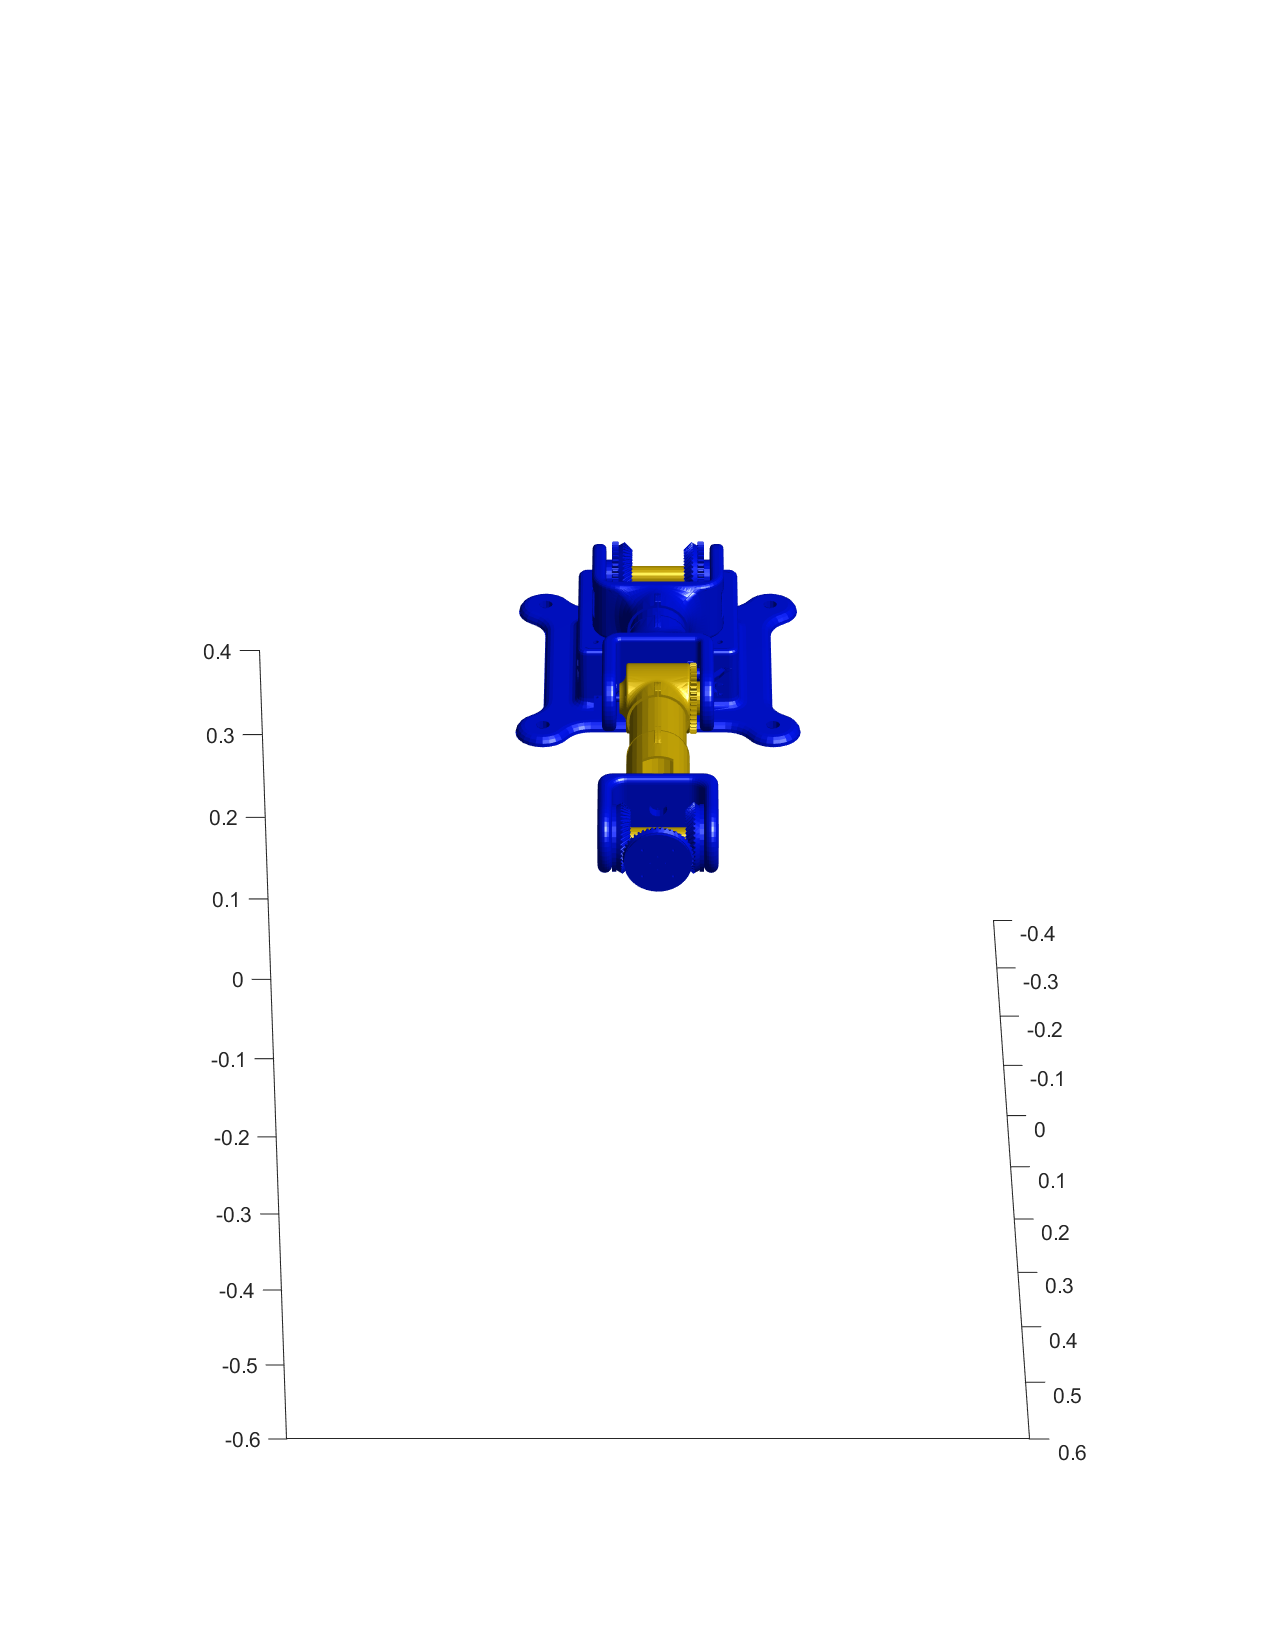
\includegraphics[width=.55\textwidth,frame]{olsnap1}
  \caption{Frame Snapshot near Simulation \\Initiation}
  \label{fig:olsnap1}
\end{subfigure}%
\begin{subfigure}[c]{0.5\textwidth}
  \center
  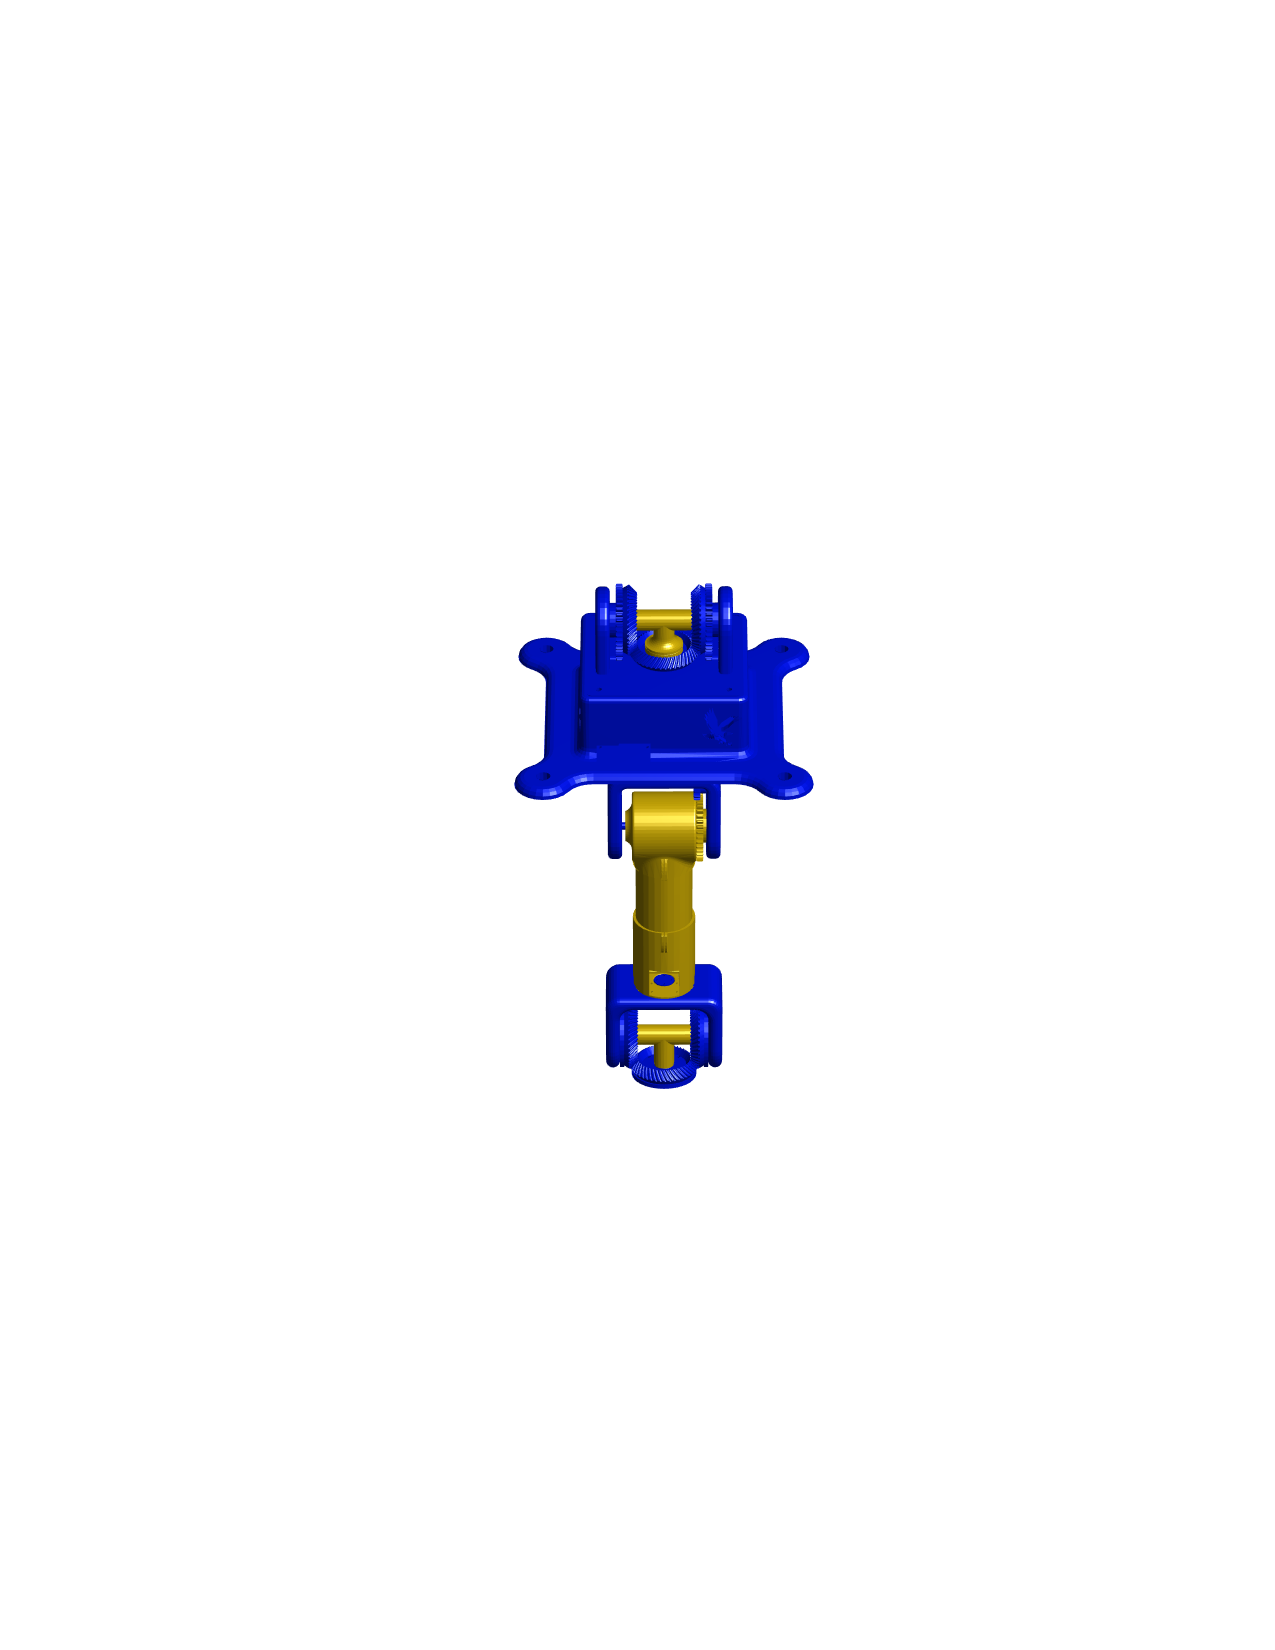
\includegraphics[width=.55\textwidth,frame]{olsnap2}
  \caption{Frame Snapshot near Simulation Termination}
  \label{fig:olsnap2}
\end{subfigure}
  \caption{Open-Loop Control Simulation Animation Snapshots}
  \label{fig:olsnaps}
\end{figure}
\looseness=-1

\begin{figure}[htp]
  \center
  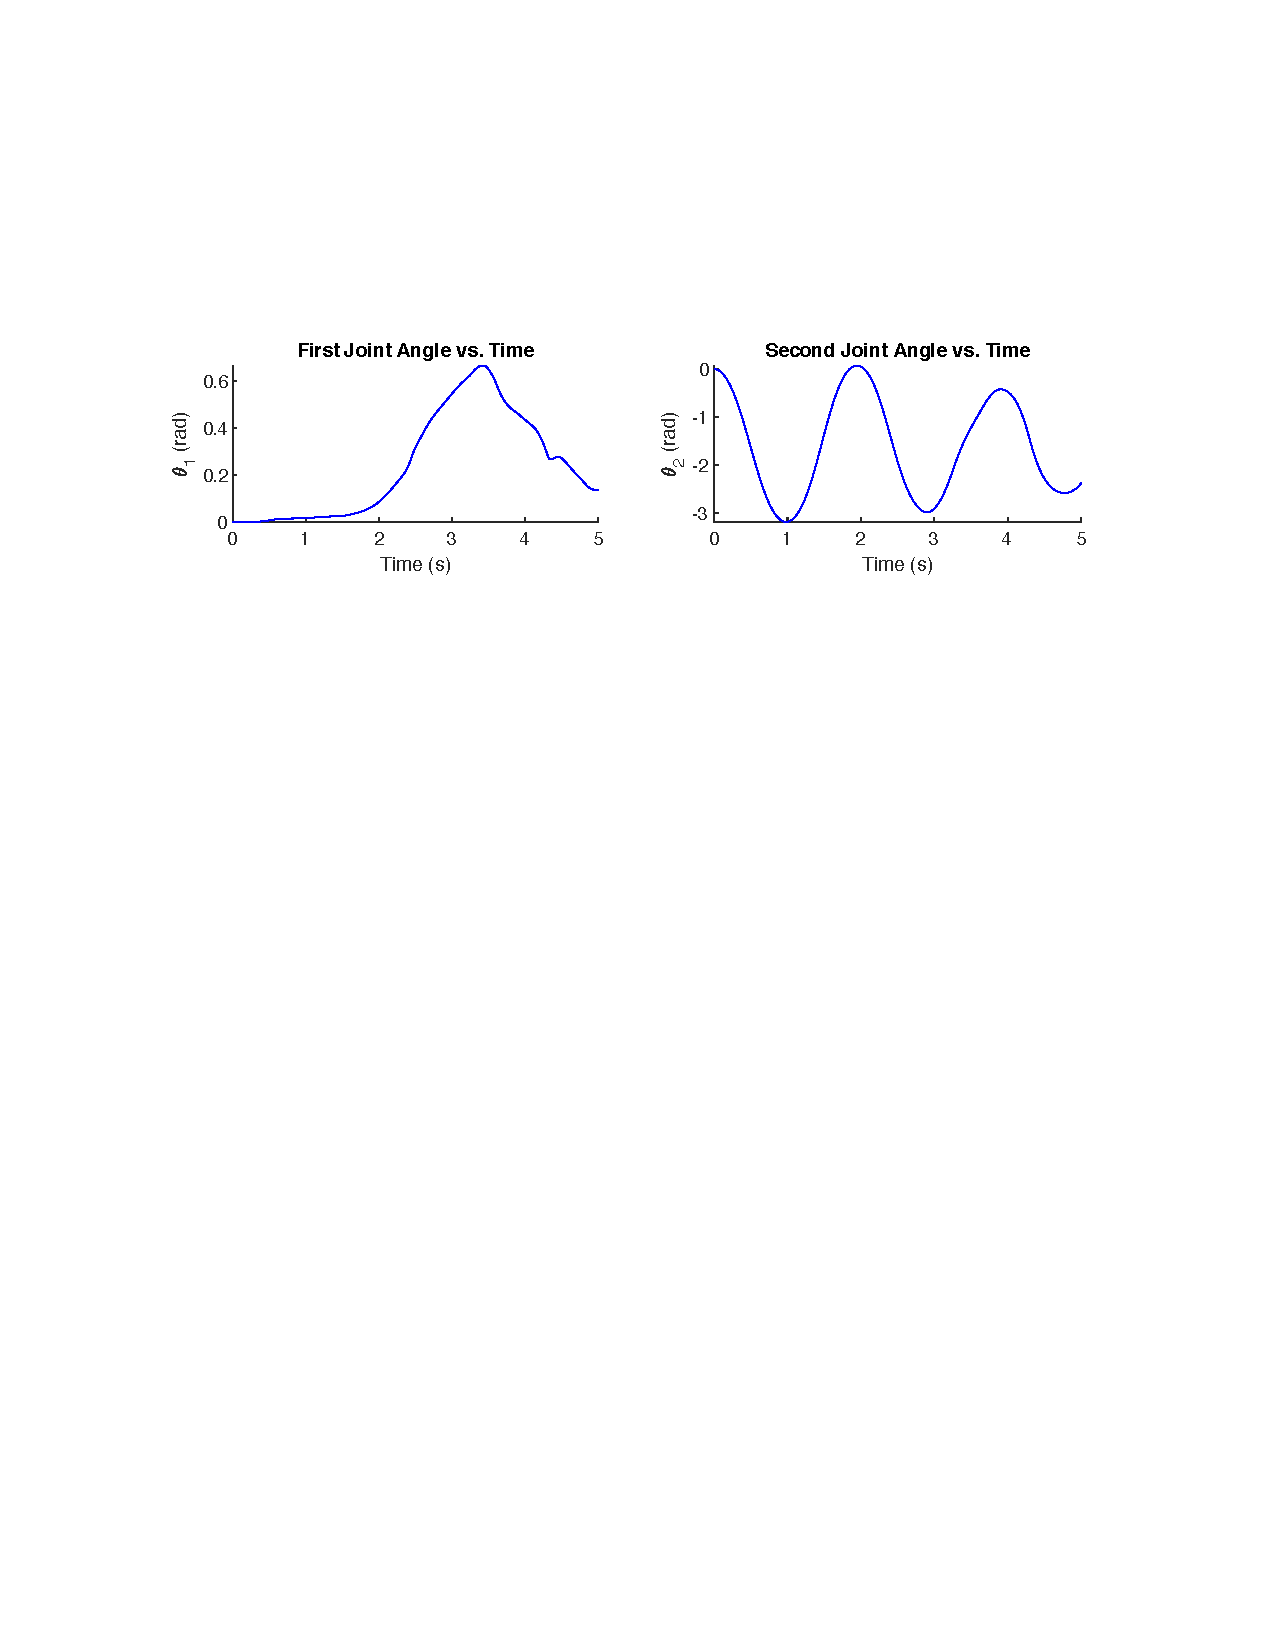
\includegraphics[width=.95\textwidth]{oljplots1}
  \caption{Joint Angles vs Time in Open-Loop Simulation}
  \label{fig:oljplots1}
\end{figure}
\begin{figure}[htp]
  \center
  \ContinuedFloat
  \captionsetup{list=off,format=cont}
  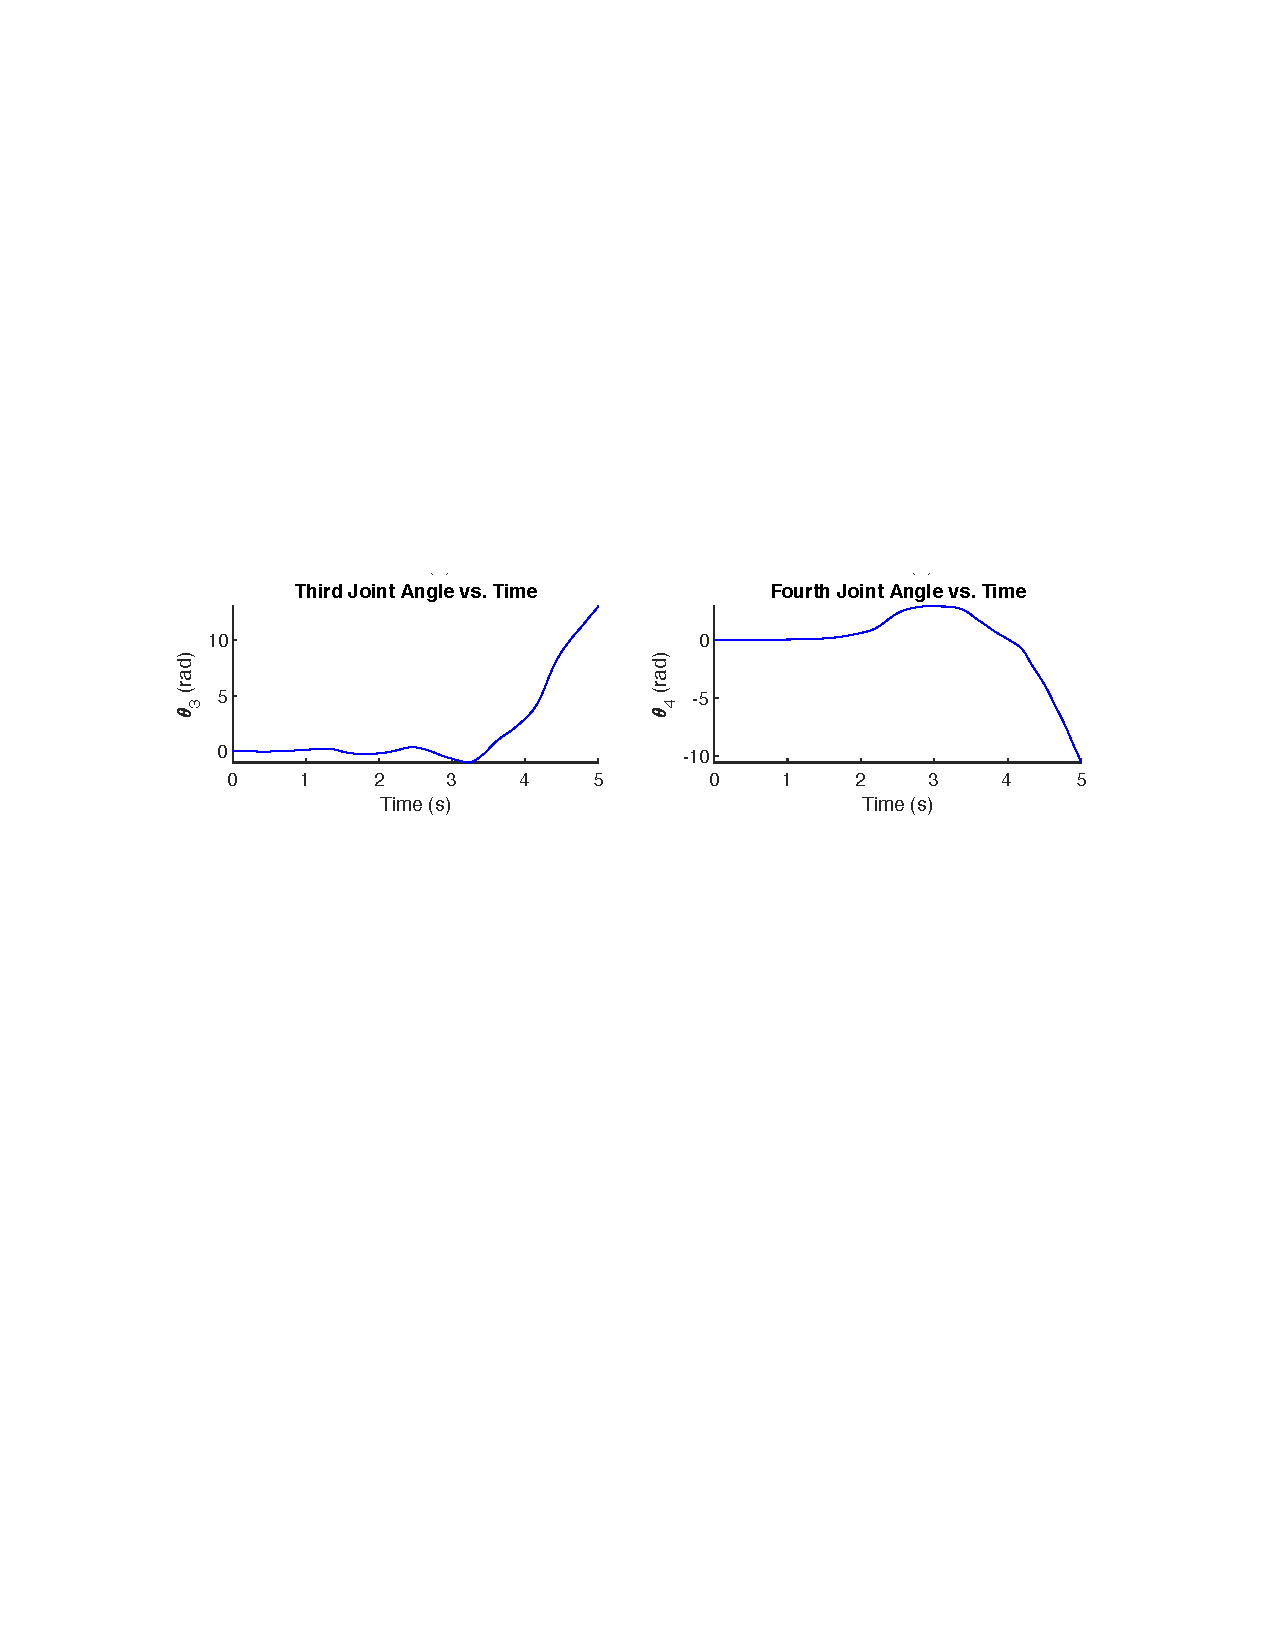
\includegraphics[width=.95\textwidth]{oljplots2}
  \caption{Joint Angles vs Time in Open-Loop Simulation}
  \label{fig:oljplots2}
\end{figure}
\begin{figure}[htp]
  \center
  \ContinuedFloat
  \captionsetup{list=off,format=cont}
  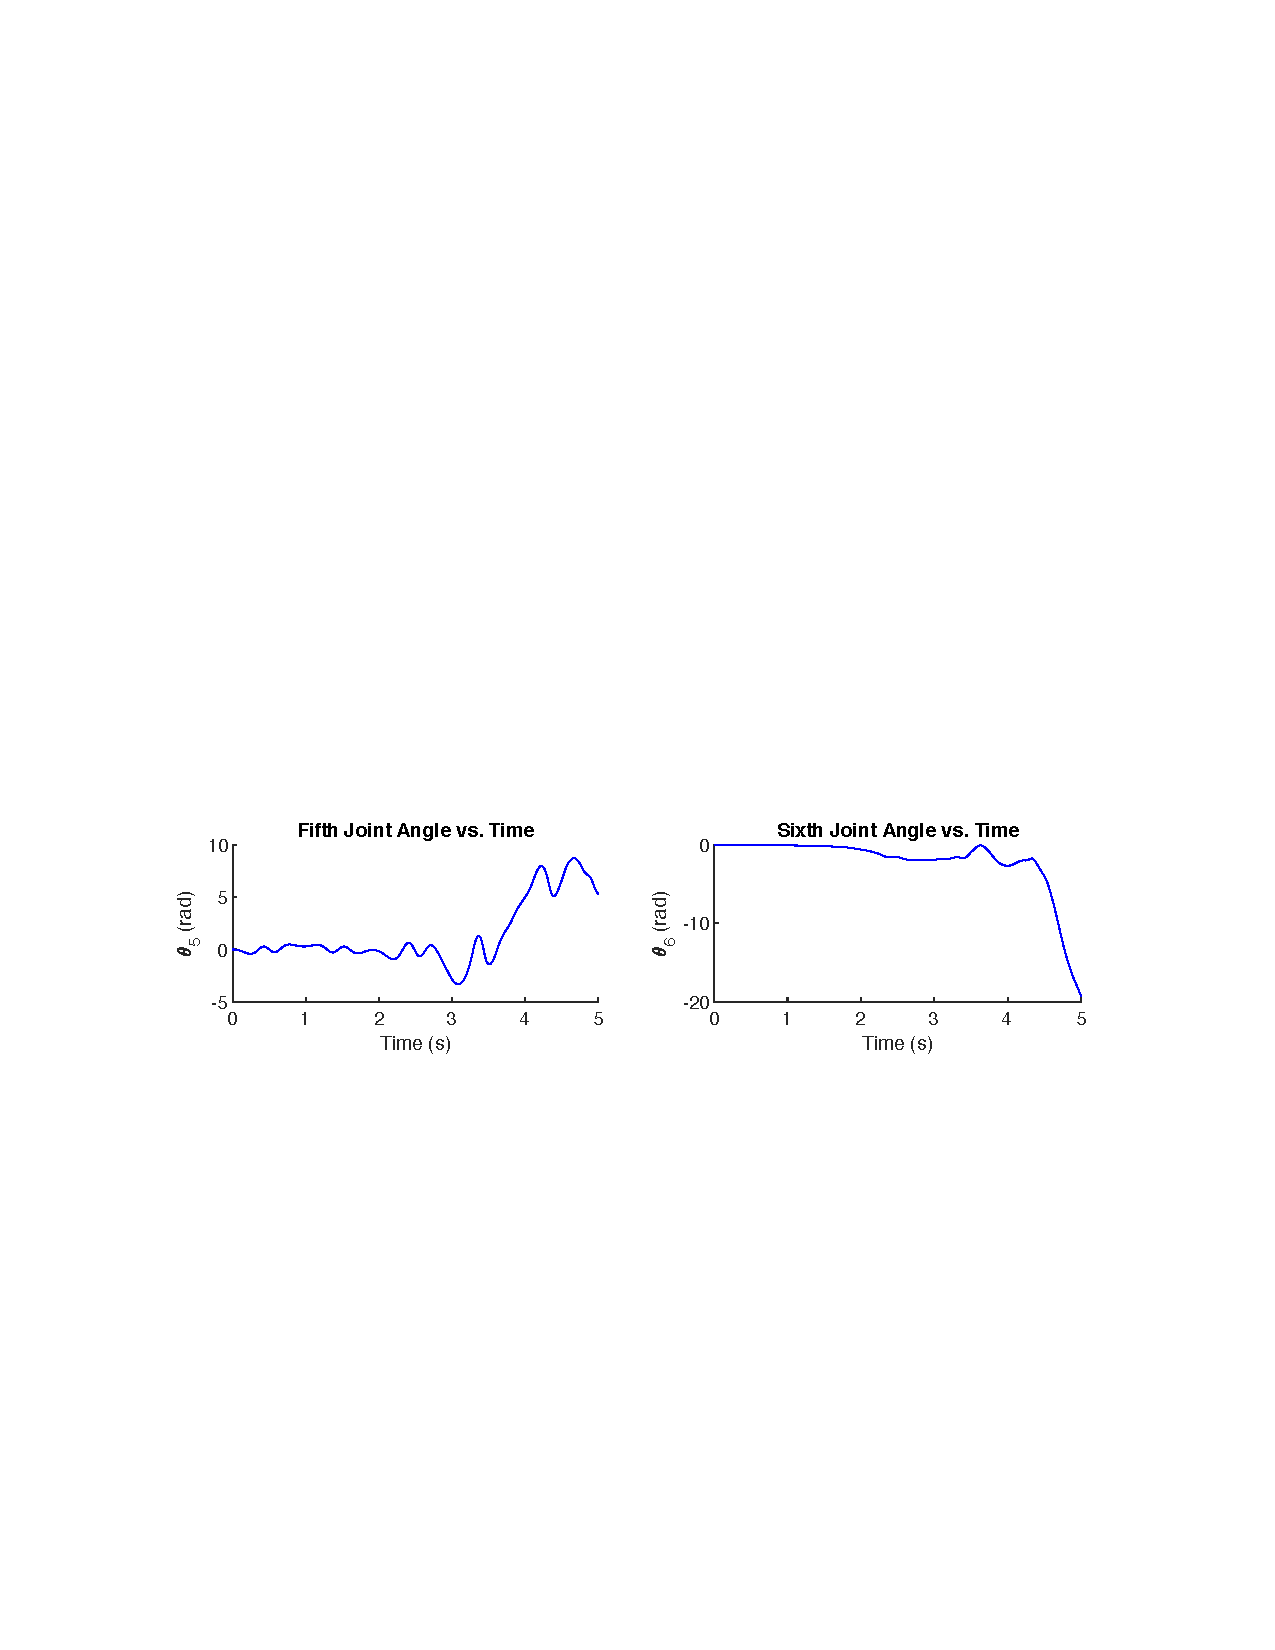
\includegraphics[width=.95\textwidth]{oljplots3}
  \caption{Joint Angles vs Time in Open-Loop Simulation}
  \label{fig:oljplots3}
\end{figure}

\newpage
\subsection{Closed-Loop Simulation}
The motor equation (\ref{eq:fin}) gives an expression for the motor torques, however the system dynamics are defined in terms of geometric joint angles. The inclusion of differential drive systems means that the joint angles, $\gamma$ do not directly correspond to motor rotations, $\theta$. However, there is a linear relation between them, described in equation (\ref{eq:A}).
\begin{equation}
  \gamma = A\theta\quad \text{where}~~A=\left[\begin{array}{cccccc}{1 /(2 N)} & {1 /(2 N)} & {0} & {0} & {0} & {0} \\ {1 /(2 N)} & {-1 /(2 N)} & {0} & {0} & {0} & {0} \\ {0} & {0} & {-1 / N} & {0} & {0} & {0} \\ {0} & {0} & {0} & {1} & {0} & {0} \\ {0} & {0} & {0} & {0} & {-1 / 2} & {1 / 2} \\ {0} & {0} & {0} & {0} & {1 / 2} & {1 / 2}\end{array}\right]
\label{eq:A}
\end{equation}
Equation (\ref{eq:A}) can be used to map the joint angles to the motor angles. The gear ratio of 1:10 is represented by the variable N. Similarly, the motor angles can be determined by multiplying both sides of equation (\ref{eq:A}) by the inverse of matrix A, giving the following relation.
\begin{equation}
\theta=A^{-1} \gamma
\label{eq:Ainv}
\end{equation}
It is important to note that the virtual work done by the joint torques ($F_{\gamma}$) and the virtual work done by the motor torques ($F_{\theta}$) are equal. Using equation (\ref{eq:Ainv}), a linear relation between the joint torques and motor torques can be determined.
\[
\begin{aligned}
  \delta W = F_{\theta}^{T} \delta \theta&=F_{\gamma}^{T} \delta \gamma, \text { where } \delta \gamma=A \delta \theta \\
  F_{\theta}^{T} \delta \theta &= F_{\gamma}^{T}(A \delta \theta) \\
  F_{\theta}^{T}&=F_{\gamma}^{T} A\\
  \left(F_{\theta}^{T}\right)^{T}&=\left(F_{\gamma}^{T} A\right)^{T}\\
  F_{\theta}=A^{T} F_{\gamma} &\Leftrightarrow F_{\gamma}=A^{-T} F_{\theta}\qquad\quad
\end{aligned}
\]
Using this equation, a relation can be determined between the motor dynamics and the system dynamics given in equation (\ref{eq:fin}) and equation (\ref{eq:eoms}) respectively.

\[
H(\gamma) \ddot{\gamma}+d(\gamma, \dot{\gamma})+G(\gamma)=-A^{-T}\left(C_1A^{-1} \ddot{\gamma}+C_2 A^{-1} \dot{\gamma}+C_3 \theta_{d}- C_3A^{-1} \gamma\right)
\]
\begin{equation}
\ddot{\gamma}=H(\gamma)^{-1}\left(-A^{-T}\left(C_1 A^{-1} \ddot{\gamma}+C_2 A^{-1} \dot{\gamma}+C_3 \theta_{d}-C_3A^{-1} \gamma\right)-d(\gamma, \dot{\gamma})-G(\gamma)\right)
\label{eq:gddot}
\end{equation}

Because this equation includes the motor model, which in turn includes an internal PD controller, this equation can be integrated to solve for the system response given a desired motor angle input, $\theta_d$. However, doing so will not result in the desired system response. This control scheme does not have any compensation for the inertia of the links, and it is also lacking gravity compensation. This can be remedied by modifying the input to the motors, $\theta_d$. A new input, $u$, is defined such that gravity can be compensated. Thus, the motor input term in equation (\ref{eq:gddot}) must include both compensation for gravity and the desired motor angle.
\[
A^{-T} C_3  u=G(\gamma)+d(\gamma, \dot{\gamma})+A^{-T} C_3\theta_{d}
\]
\begin{equation}
u=\left(A^{-T} C_3\right)^{-1} \left(G(\gamma)+d(\gamma, \dot{\gamma})\right) + \theta_{d}
\end{equation}
With this new motor input, the closed loop control system equations of motion are given as:
\begin{equation}
\ddot{\gamma}=H(\gamma)^{-1}\left(-A^{-T}\left(C_1 A^{-1} \ddot{\gamma}+C_2 A^{-1} \dot{\gamma}+C_3 u-C_3A^{-1} \gamma\right)-d(\gamma, \dot{\gamma})-G(\gamma)\right)
\label{eq:gddotfin}
\end{equation}
Equation (\ref{eq:gddotfin}) can then be integrated to solve for the system response given desired motor angles.

\begin{figure}[htp]
  \center
  \begin{subfigure}[c]{0.33\textwidth}
    \center
    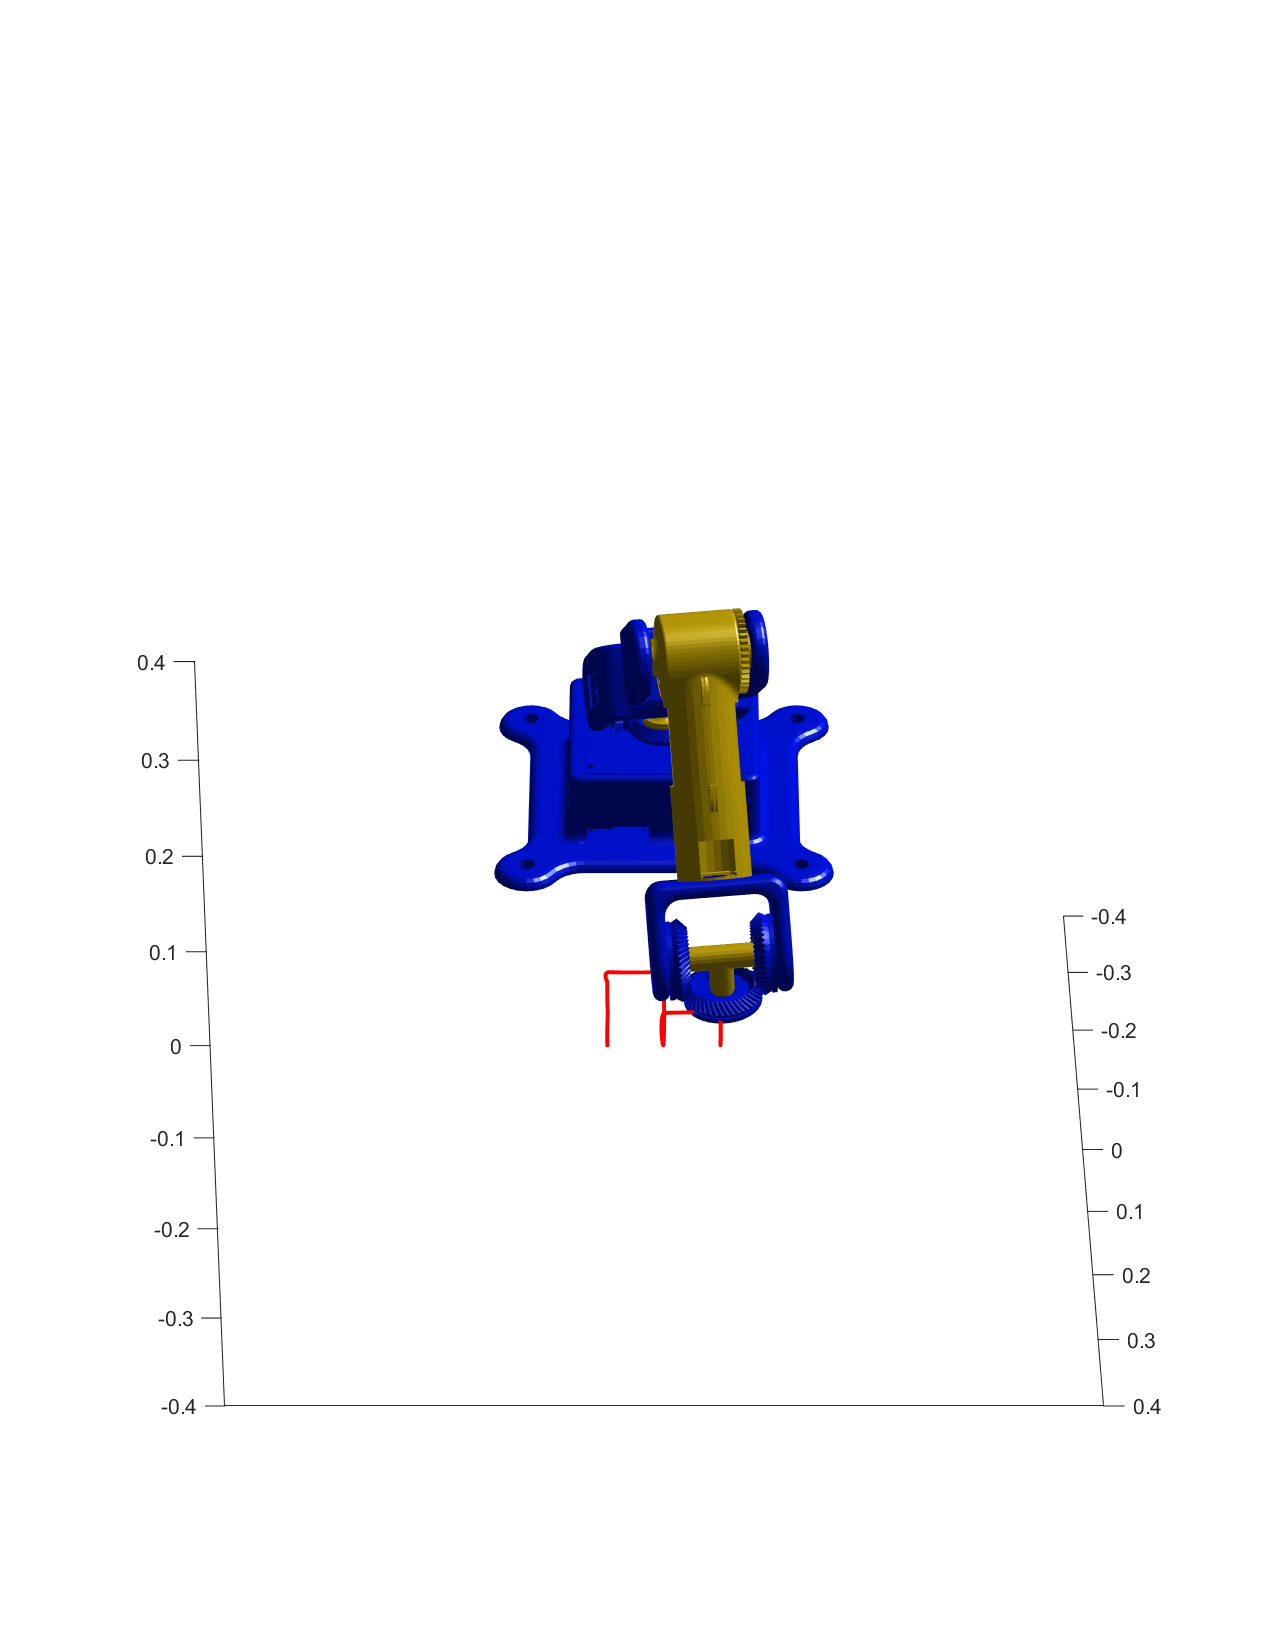
\includegraphics[width=.9\textwidth,frame]{clsnap1}
    \caption{Frame Snapshot near Simulation \\Initiation}
  \end{subfigure}%
  \begin{subfigure}[c]{0.33\textwidth}
    \center
    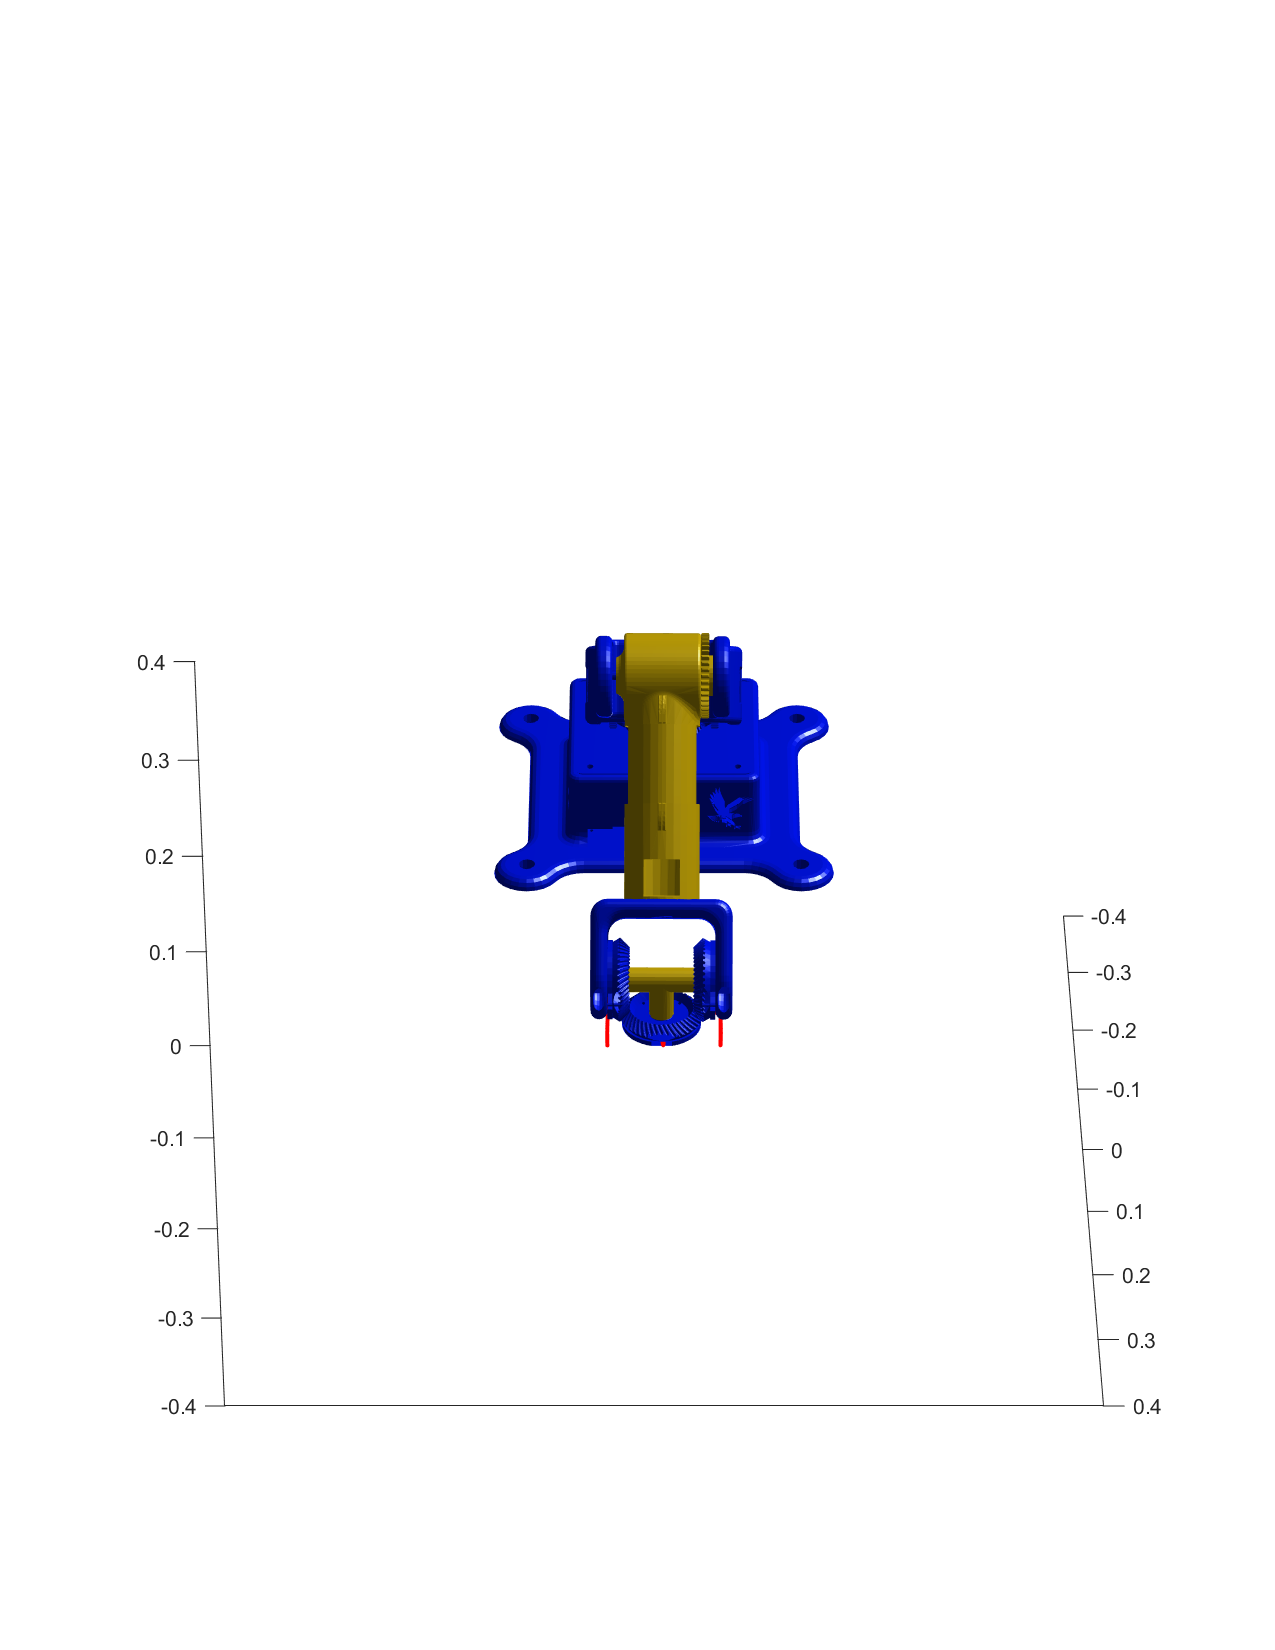
\includegraphics[width=.9\textwidth,frame]{clsnap2}
    \caption{Frame Snapshot near Simulation \\Middle}
  \end{subfigure}%
\begin{subfigure}[c]{0.33\textwidth}
  \center
  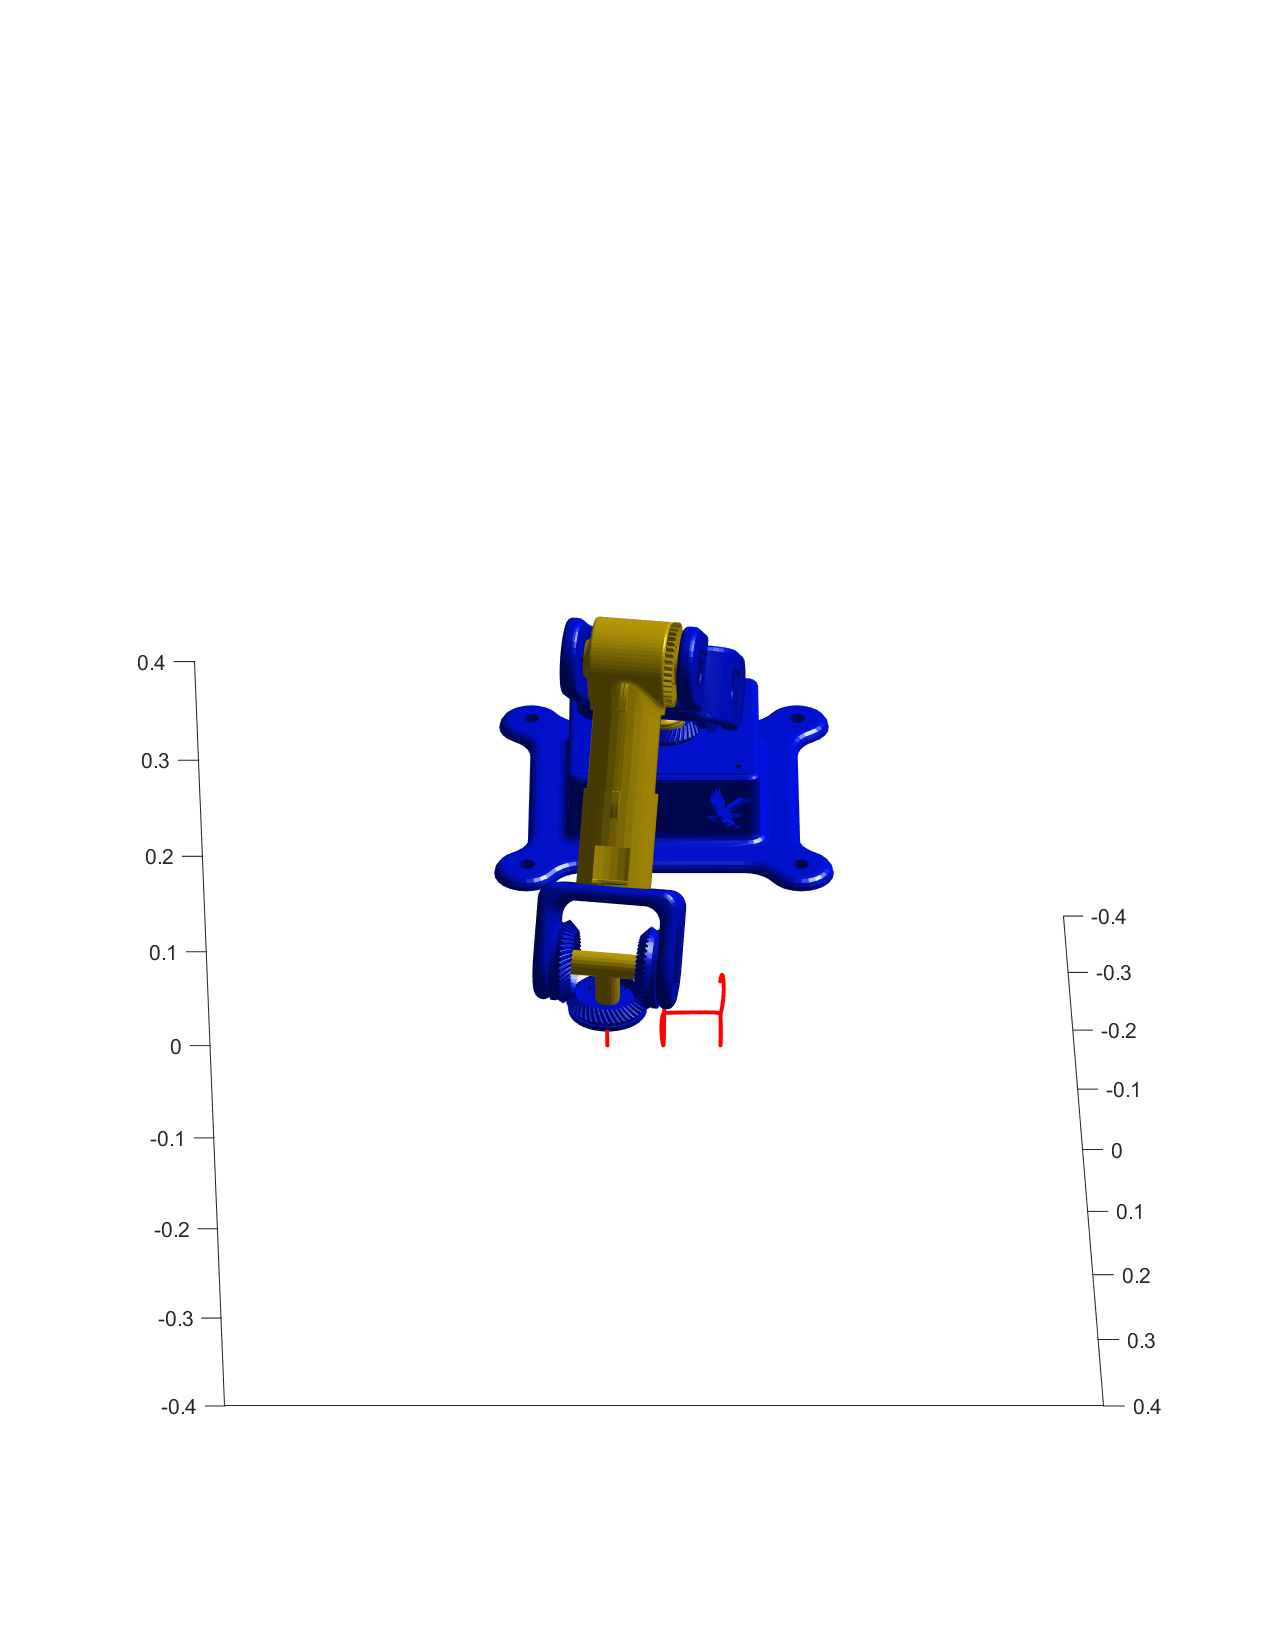
\includegraphics[width=.9\textwidth,frame]{clsnap3}
  \caption{Frame Snapshot near Simulation \\Termination}
\end{subfigure}
  \caption{Closed-Loop Control Simulation Animation Snapshots}
  \label{fig:clsnaps}
\end{figure}

% The closed-loop system can now be simulated, the results are shown below in Figure (\ref{fig:jplots}).
\begin{figure}[htp]
  \center
  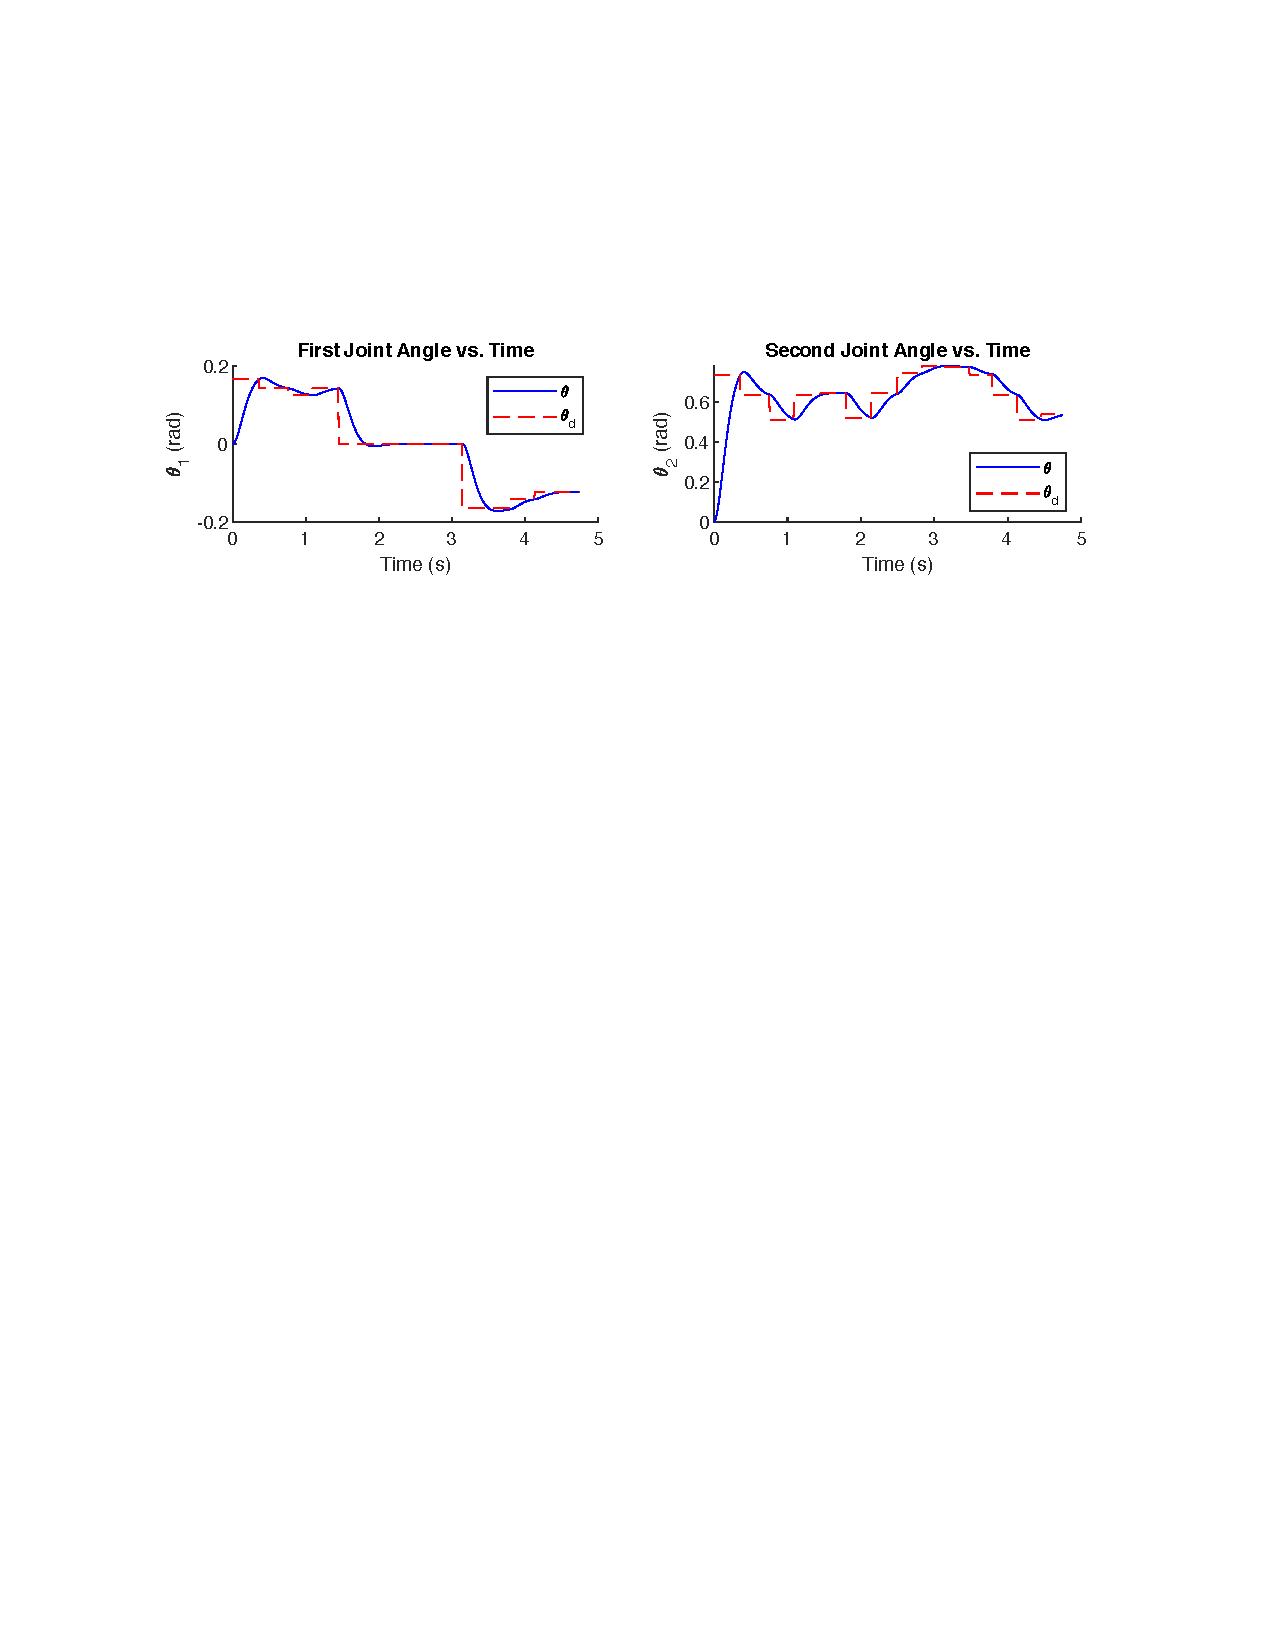
\includegraphics[width=.95\textwidth]{cljplots1}
  \caption{Joint Angles vs Time in Closed-Loop Simulation}
  \label{fig:cljplots1}
\end{figure}
\begin{figure}[htp]
  \center
  \ContinuedFloat
  \captionsetup{list=off,format=cont}
  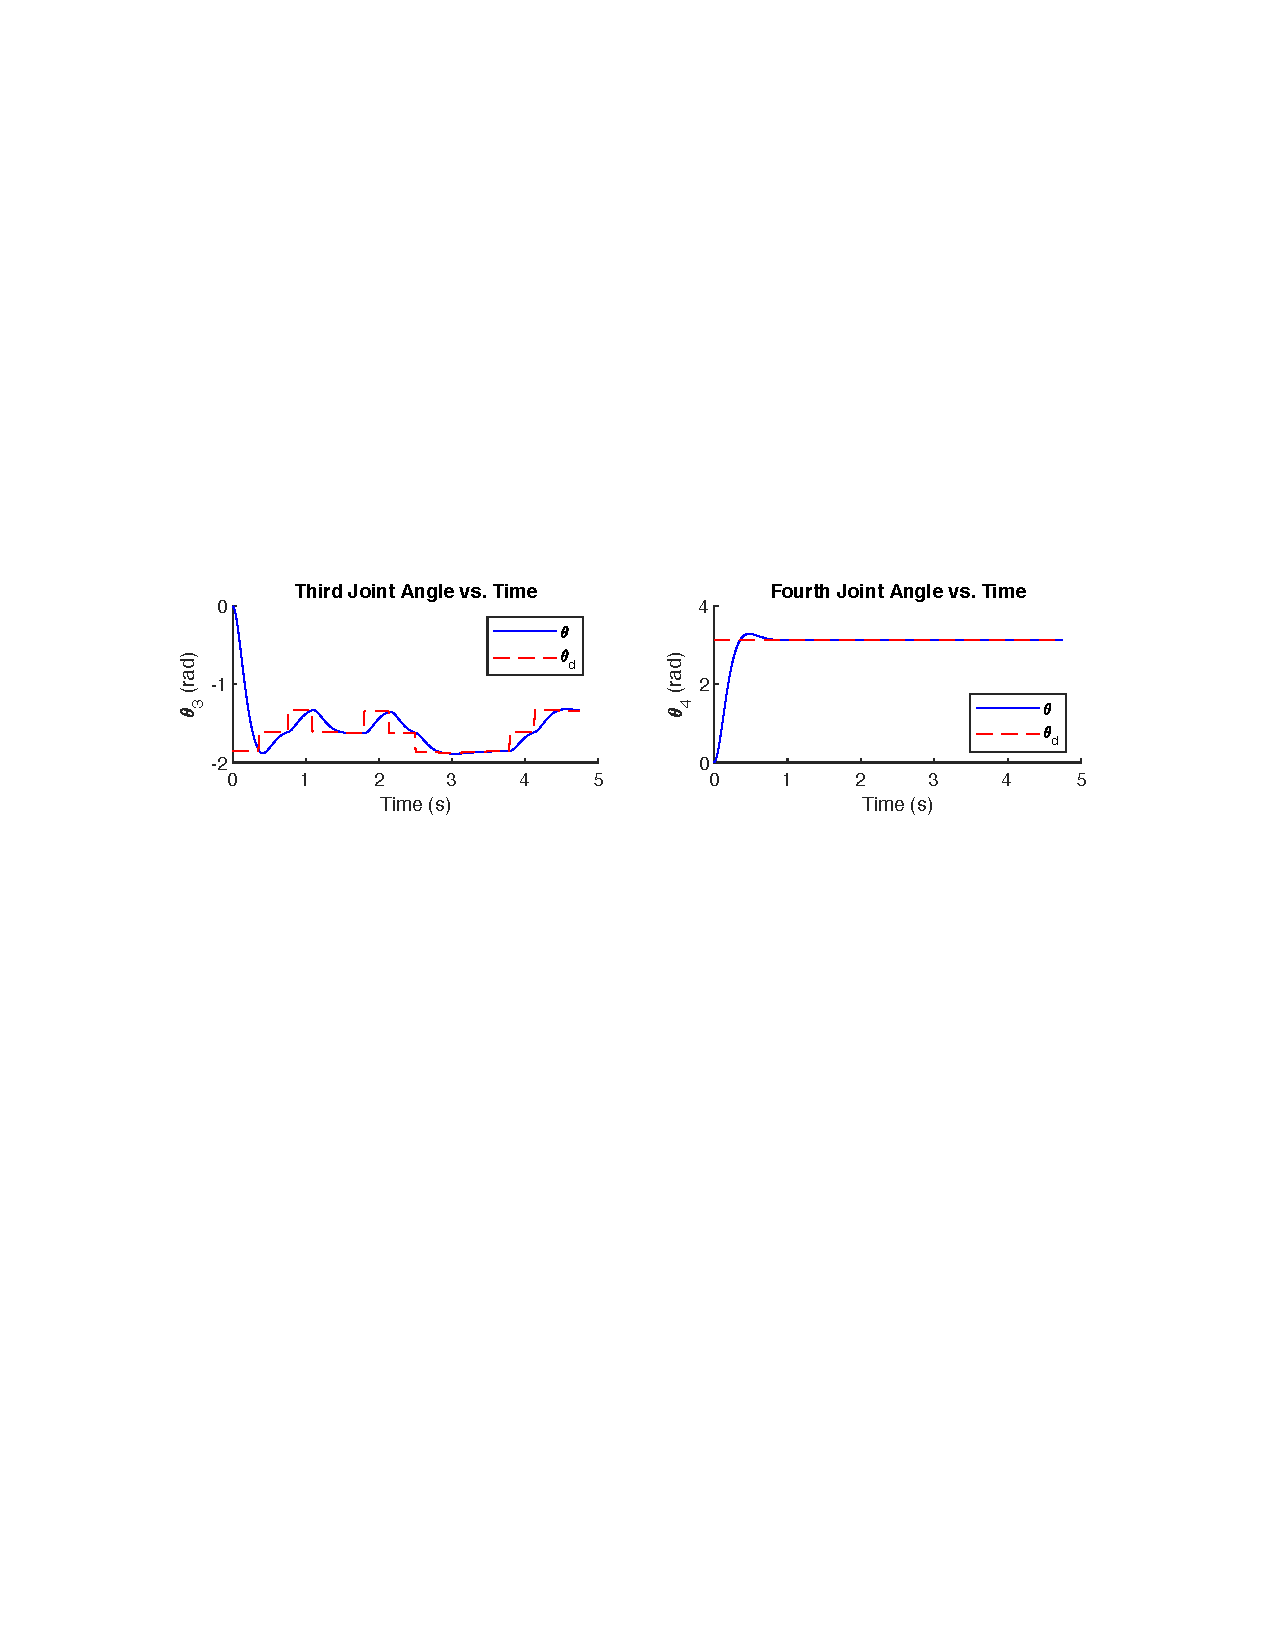
\includegraphics[width=.95\textwidth]{cljplots2}
  \caption{Joint Angles vs Time in Closed-Loop Simulation}
  \label{fig:cljplots2}
\end{figure}
\begin{figure}[htp]
  \center
  \ContinuedFloat
  \captionsetup{list=off,format=cont}
  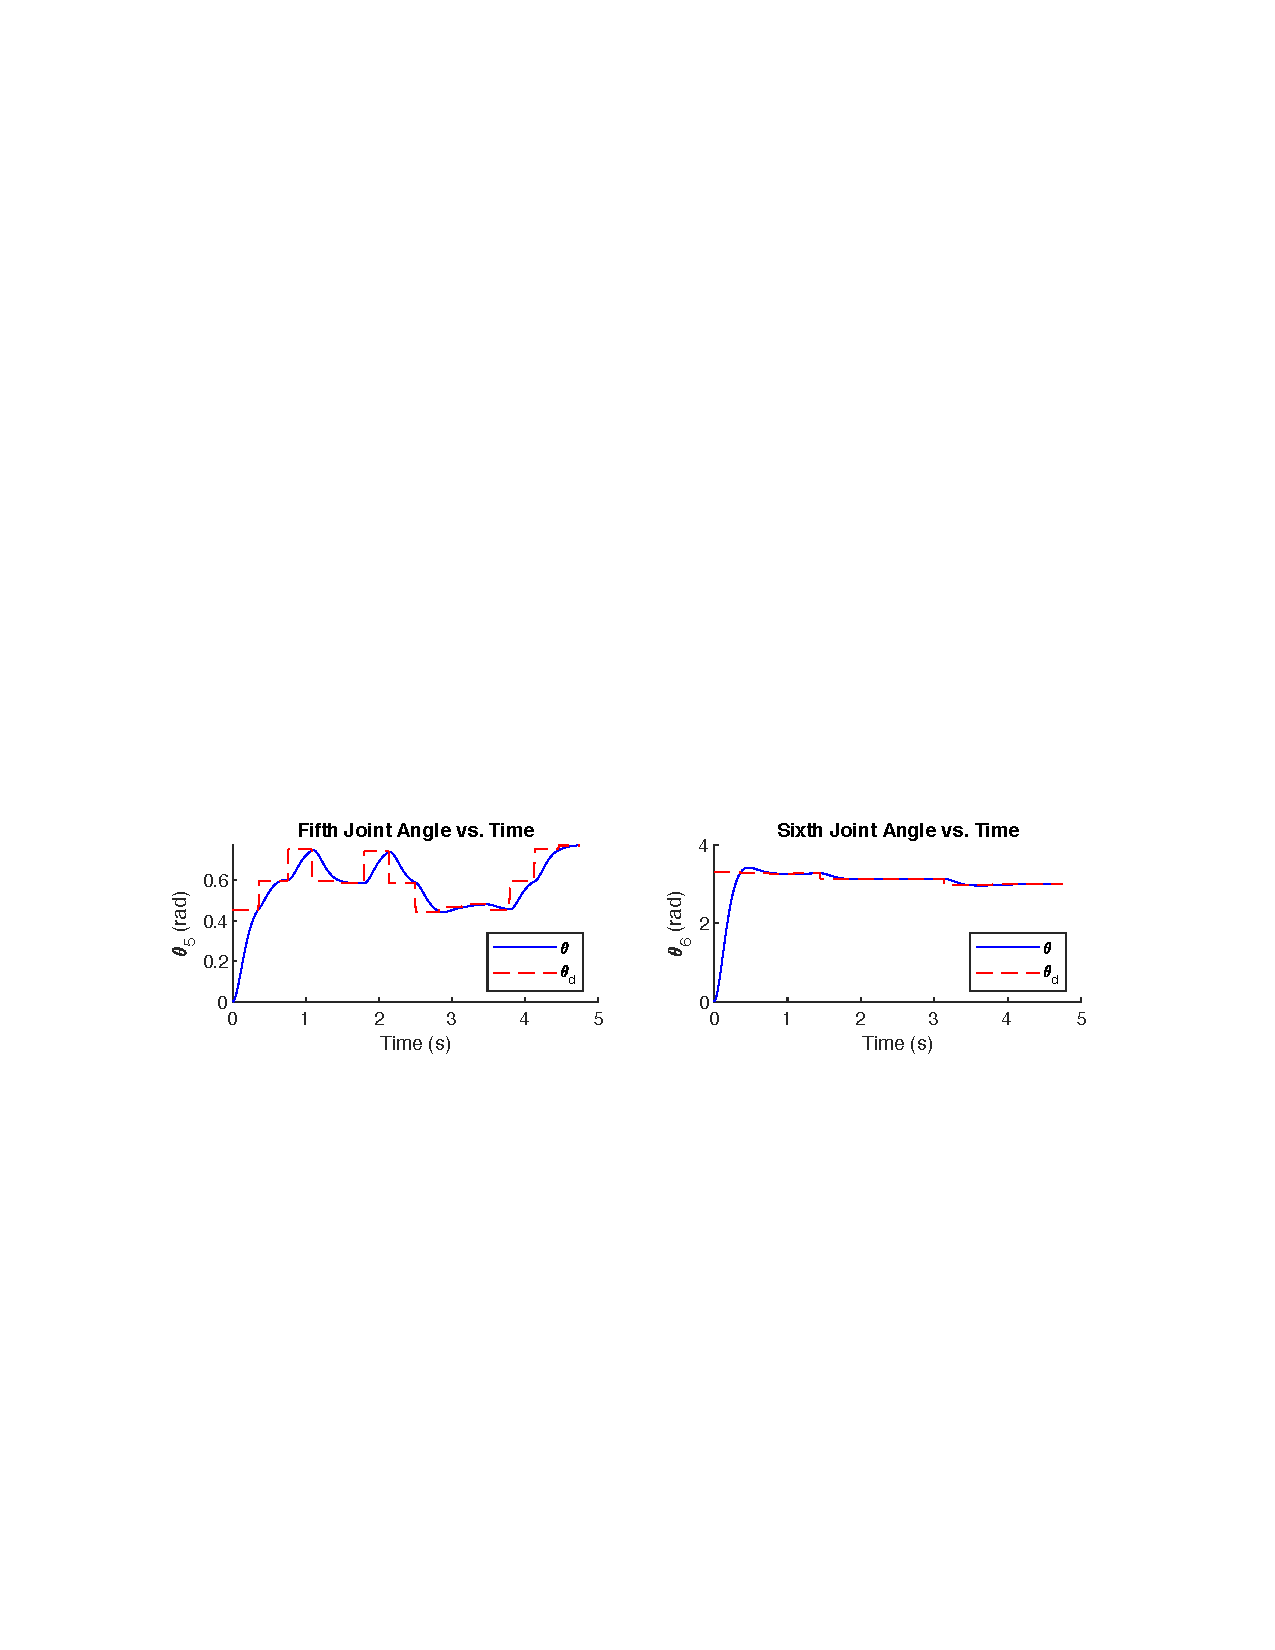
\includegraphics[width=.95\textwidth]{cljplots3}
  \caption{Joint Angles vs Time in Closed-Loop Simulation}
  \label{fig:cljplots3}
\end{figure}

\newpage
\subsection{ANSYS}
With 100\% infill, 3D printed PLA has a maximum shear stress of 13.6 kpsi. The manipulator applies a load of 13N in the negative y-direction. Without gears in the base differential, the differential support would bear the load on its bearing mounts. \emph{Figure \ref{fig:tbar}} shows the manipulator’s differential support could experience up to 97 kPa or 0.014 kpsi of shear stress, which is less than the maximum shear stress of PLA with 100\% infill. Since some of the manipulator’s mass is supported by the gears, the actual shear experienced by the differential support will be less.

\begin{figure}[htp]
  \center
  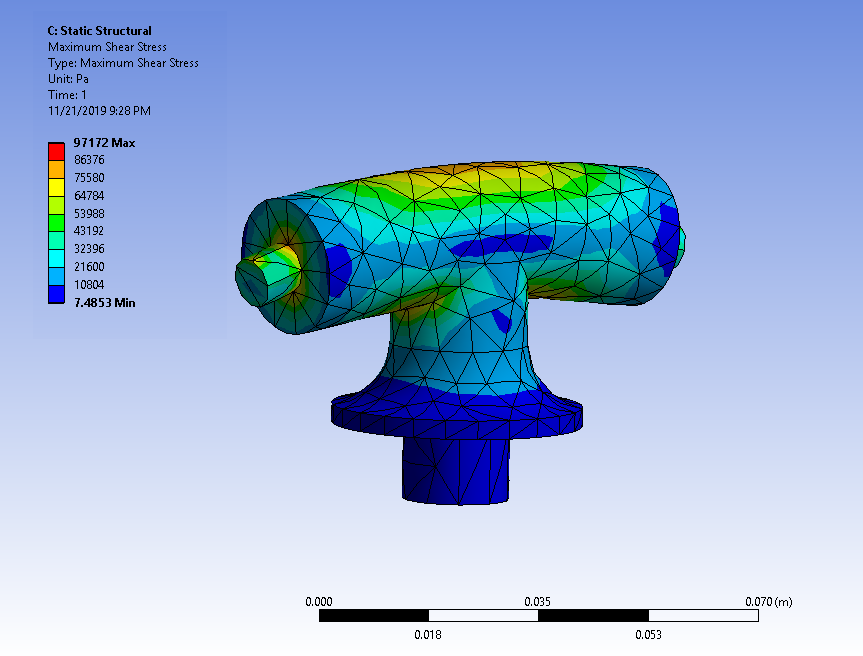
\includegraphics[width=.99\textwidth, frame]{tbar}
  \caption{T-Bar ANSYS FEA}
  \label{fig:tbar}
\end{figure}

To simulate a dynamical loading situation where the manipulator would be under the largest amount of stress, gravitational forces and an outward force (parallel to the arm direction in it's zeroed configuration) were applied to the structure. This situation represents the worst-case loading scenario, such as the manipulator swinging while outstretched. The supports and simulated forces can be seen in the ANSYS image capture shown in \emph{Figure \ref{fig:ansys_forces}}. \\

\begin{figure}[htp]
  \center
  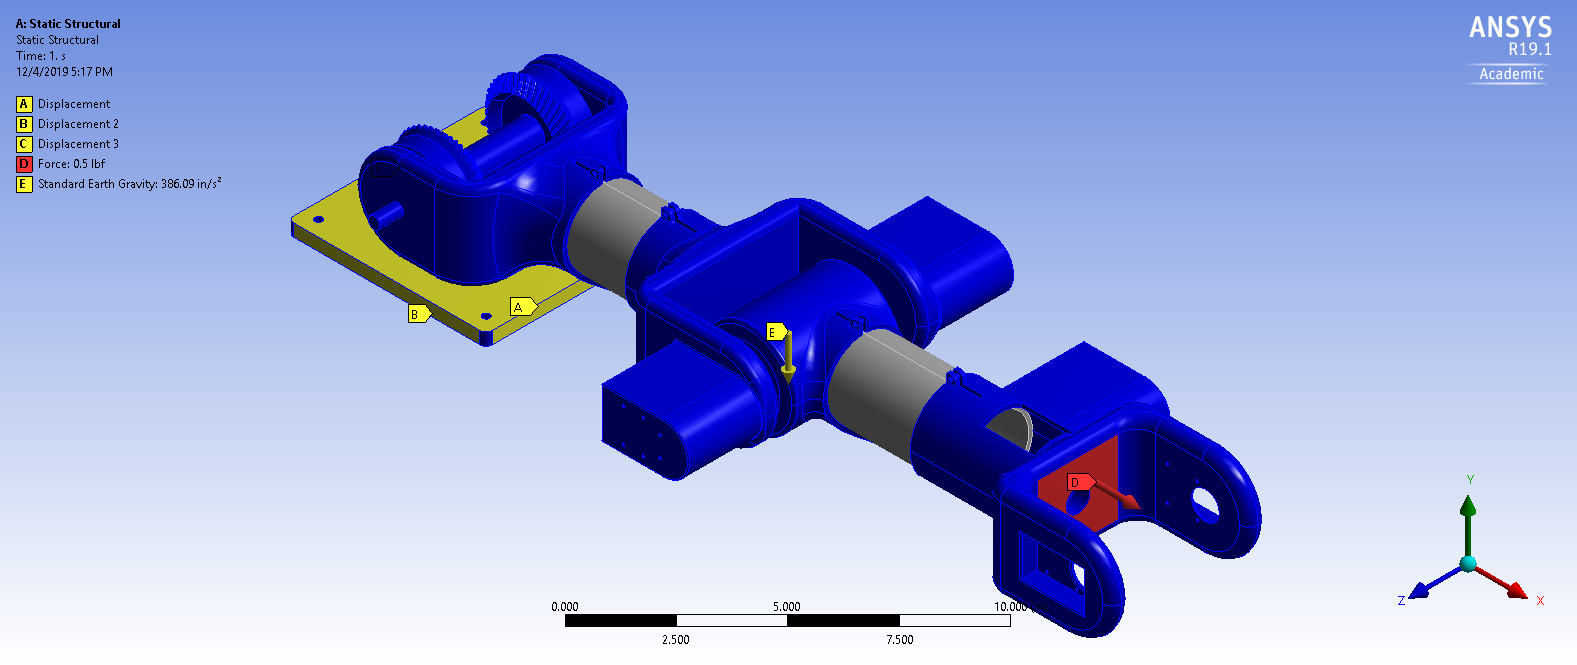
\includegraphics[width=.99\textwidth, frame]{ansys_forces}
  \caption{ANSYS Simulated Forces Image Capture}
  \label{fig:ansys_forces}
\end{figure}
As shown in \emph{Figure \ref{fig:ansys_forces}}, the red arrow is the outward force simulating centrifugal forces, the yellow arrow represents gravity acting at the manipulator's center of mass, and the yellow highlighted faces show the fixed support at the base.

The dynamical loadings resulted in a maximum shear stress at the shoulder differential bearing, as seen in \emph{Figure \ref{fig:ansys_full}}; a close-up image of the bearing analysis can be seen in \emph{Figure \ref{fig:ansys_bearing}}.

\begin{figure}[htp]
  \center
  \begin{subfigure}[t]{0.5\textwidth}
  \center
  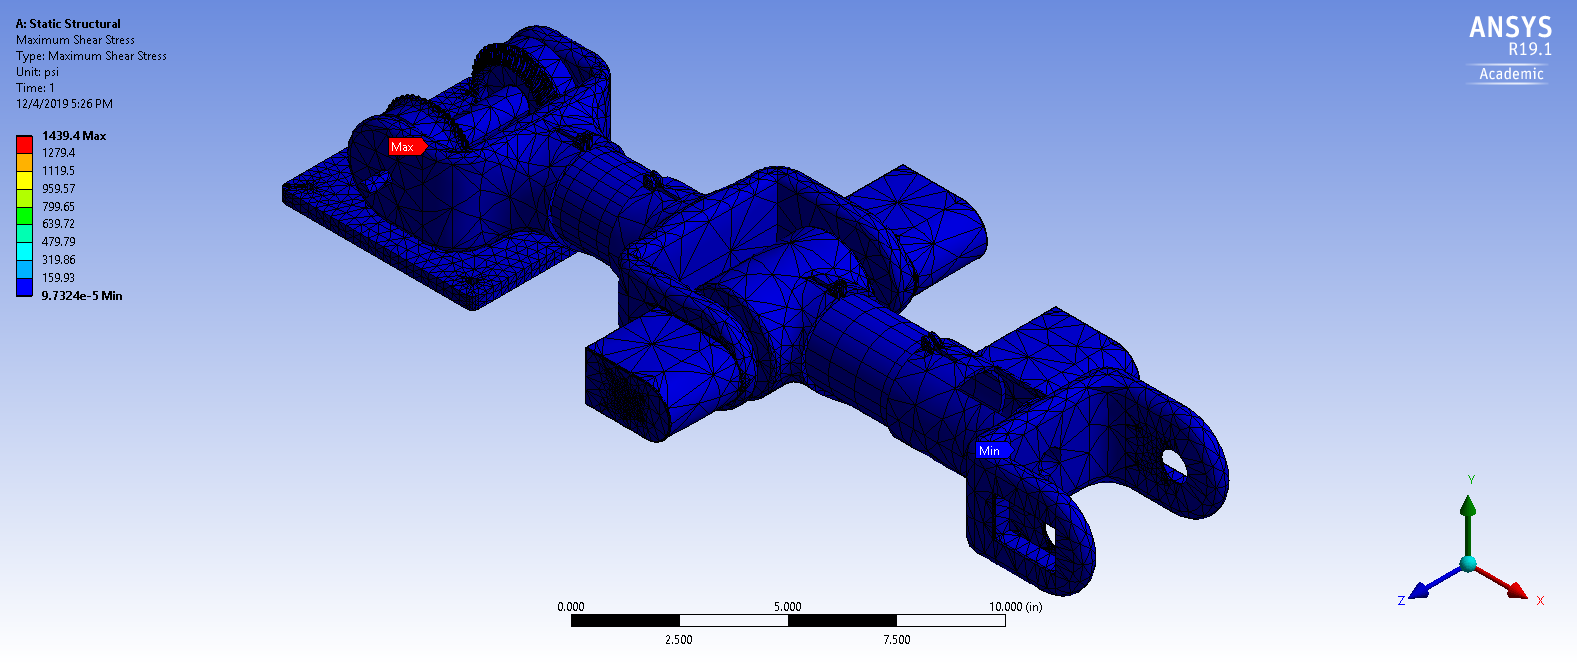
\includegraphics[width=.9\textwidth,frame]{ansys_full}
  \caption{ANSYS Full View of Maximum Shear}
  \label{fig:ansys_full}
\end{subfigure}%
\begin{subfigure}[t]{0.5\textwidth}
  \center
  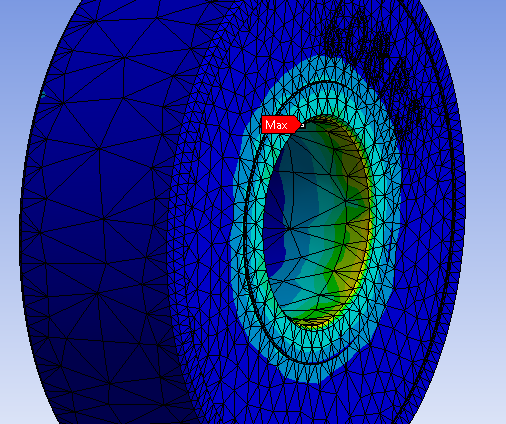
\includegraphics[width=.75\textwidth,frame]{ansys_bearing}
  \caption{ANSYS Bearing Shear Stress Close-up}
  \label{fig:ansys_bearing}
\end{subfigure}
  \caption{ANSYS FEA of Dynamical Loading Scenario}
\end{figure}

To further validate that the structure is capable of handling alternating stresses, a fatigue test was also performed showing the life of the manipulator handles a minimum of 1e6 cycles, as seen in \emph{Figure \ref{fig:ansys_life}}, showing it is unlikely to fail due to material yeilding.
\newpage

\begin{figure}[htp]
  \center
  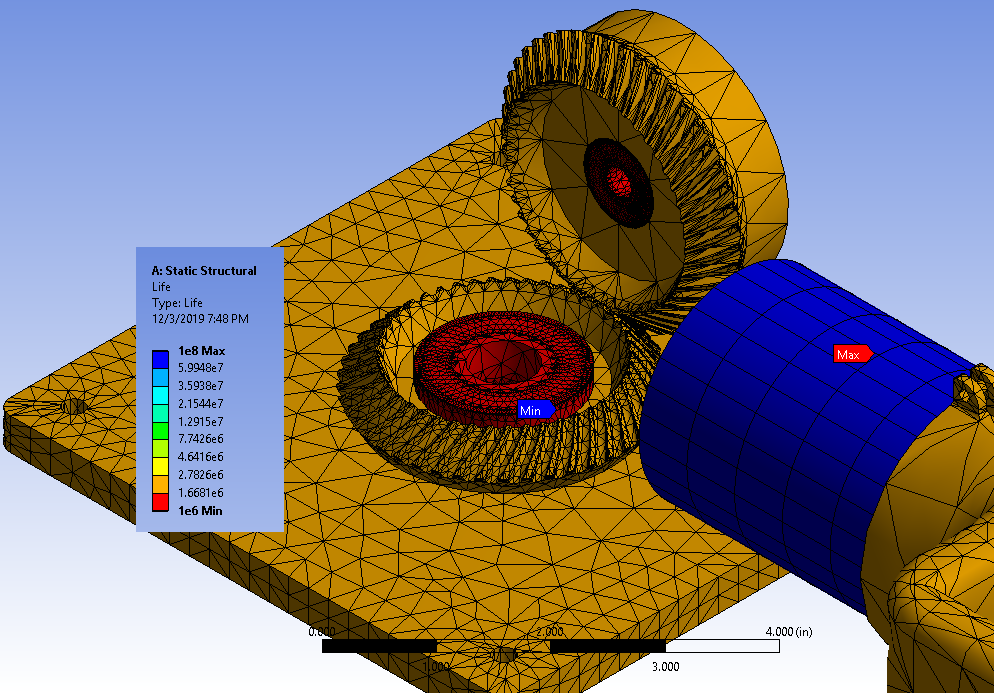
\includegraphics[width=.99\textwidth, frame]{ansys_life}
  \caption{ANSYS Fatigue Test}
  \label{fig:ansys_life}
\end{figure}

As seen in \emph{Figure \ref{fig:ansys_life}}, the lower bearing of the differential drive on the shoulder of the manipulator would be the most likely component to fail under repeating loadings.
\newpage
\subsection{Electrical Schematic}
The electrical schematic shown in \emph{Figure \ref{fig:eschem}} consists of a power supply that receives 120V AC that is standardly supplied from wall outlets. The Power supply has two outputs, a 5V terminal that has a max current output of 3A, and a 12V terminal that has a max output of 7A. The Raspberry Pi 3B is powered by the 5V terminal, and since the max current draw from the Pi is 1.2A the maximum current draw from the terminal is not surpassed. The six MX-12W servos used in the manipulator, as well as the AX-12A servo used in the end effector, are connected in parallel across the 12V terminal from the power supply. Since the MX-12W has a stall current of .6A and the AX-12A has a stall current of 1.5A, the maximum current to be pulled from the 12V terminal would be 5.1A, less than the 7A the supply can output. In order to communicate to the servos, a U2D2 communication converter is connected to the Raspberry Pi which creates a serial connection used by the servos, allowing the servos to be daisy-chained together. The Raspberry Pi also connects to an external PC so that the user can communicate with the Pi using a mouse, keyboard, and monitor.
\vfill
\begin{figure}[htp]
  \centering
  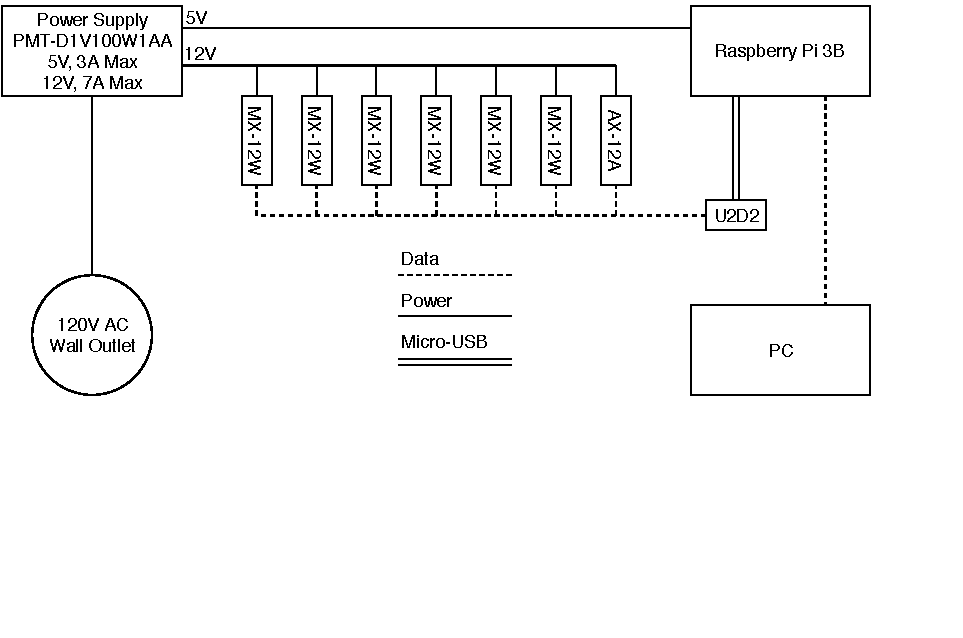
\includegraphics[width=.95\textwidth]{eschem}
  \caption{Electrical Schematic}
  \label{fig:eschem}
\end{figure}
\vfill\null
\newpage
\subsection{Software Flowchart}
% The software the system will need will take in a row vector of position, orientation, path type, and end effector function information for all points to be traveled through and run the manipulator through the desired points following the specified paths requested. To do this, the user will first be asked what the number of points being input will be so that a few data structures can be preallocated. The user will then be asked if the manipulator will be writing or doing pick and place, and store the response. If the user is doing pick and place, the user will be asked for the full point data consisting of the x, y, and z location in millimeters, the phi, theta, and psi angles in degrees, the path type, and the end effector function. If the user is doing writing, only the x, y, and z locations will be requested. The orientation of the point will be defaulted in the “down” orientation since the marker will be held vertically, the path type will be set to cartesian straight line, and the end effector function will be set to stay unchanged. When all the desired points have been input, the software will then create intermediate points every centimeter between points whose paths are specified as cartesian straight line and store the new path points in a different data structure. After the path has been created, each point will be run through inverse kinematics to get the required joint angles to achieve the position and will be stored as the motor data for each point. If the user is writing with the manipulator, the user will be prompted to press a key to close the end effector to grab the marker. The user will then be prompted to press a key to begin, at which point the software will send the motor data to each servo for the first point that the system is trying to reach, wait till the servos are in the desired position, run the end effector function if there is one, and then repeat the process with the next set of motor data until all the points have been traveled through. When the last point has been reached, the program will prompt the user to input the number of desired points and wait for the input to start the process over again.

The software the system uses takes in a row vector of position, orientation, path type, and end effector function information for all points to be traveled through and runs the manipulator through the desired points following the specified paths requested. The general overview of the code is shown in \emph{Figure \ref{fig:soverall}}.

\begin{figure}[htp]
  \center
  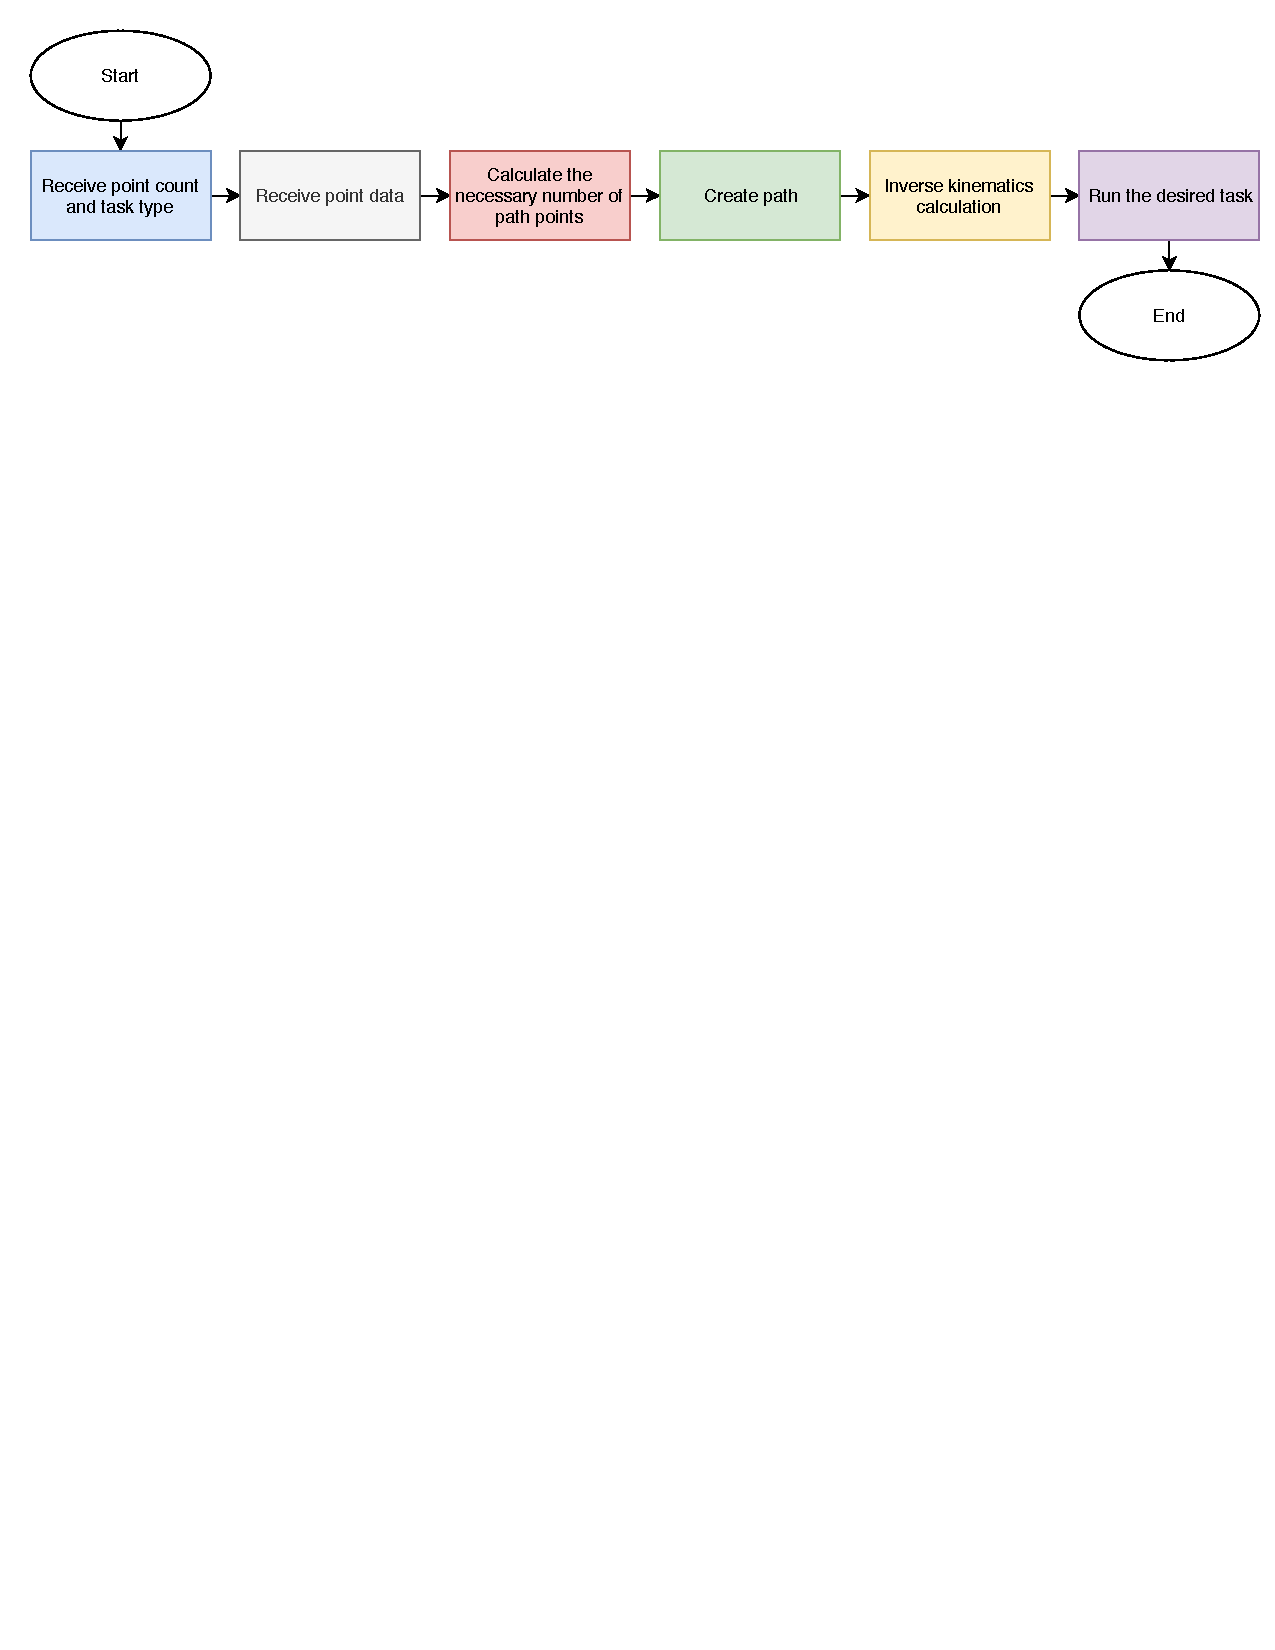
\includegraphics[width=\textwidth]{soverall}
  \caption{Software Flowchart}
  \label{fig:soverall}
\end{figure}

\emph{Figure \ref{fig:soverall}} shows that the software for the manipulator is broken up into six subsections, two sections that receive data, three that do calculations, and one that runs the specified task.

The first subsection of the software works to receive the number of points the user is inputting as well as the general task the user is completing, shown in \emph{Figure \ref{fig:sf1}}. \\

\begin{figure}[htp] \ContinuedFloat
  \begin{subfigure}[c]{\textwidth}
  \center
  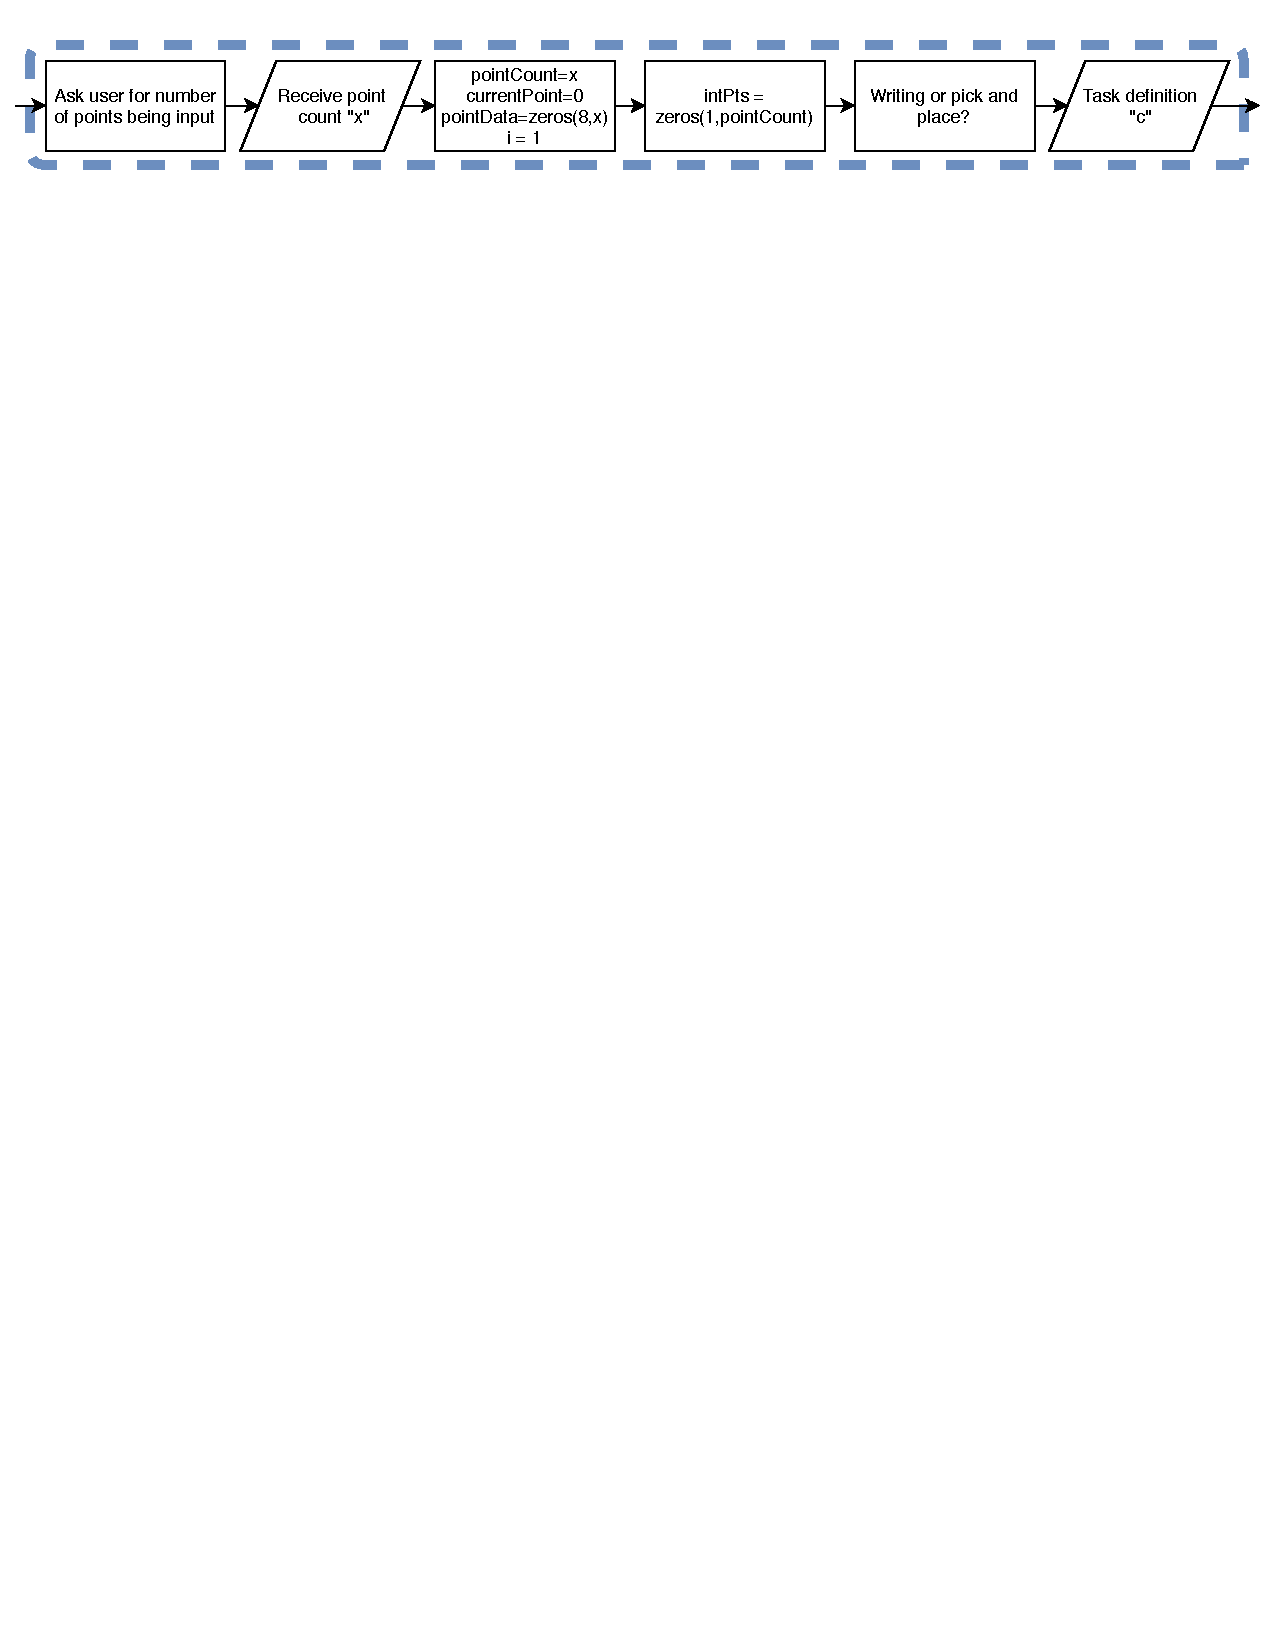
\includegraphics[width=\textwidth]{sf1}
  \caption{Software Flowchart Subsection 1}
  \label{fig:sf1}
  \end{subfigure}
\end{figure}

\emph{Figure \ref{fig:sf1}} specifies that the software prompts the user for the number of points that the manipulator will travel through and stores the input as a variable, in this case ‘x’. The ‘x’ variable is only used to help preallocate data vectors so that the size of the vector does not change with each input. The software also receives the task specification as either a 0 for cartesian straight line pathing or a 1 for a straight line in the joint space and stores this value in the variable ‘c’.

The second general block in the software flowchart works to receive and store the necessary data for the points the user is inputting depending on the path type as seen in \emph{Figure \ref{fig:sf2}}.
\newpage
\begin{figure}[htp] \ContinuedFloat
  \begin{subfigure}[c]{\textwidth}
  \center
  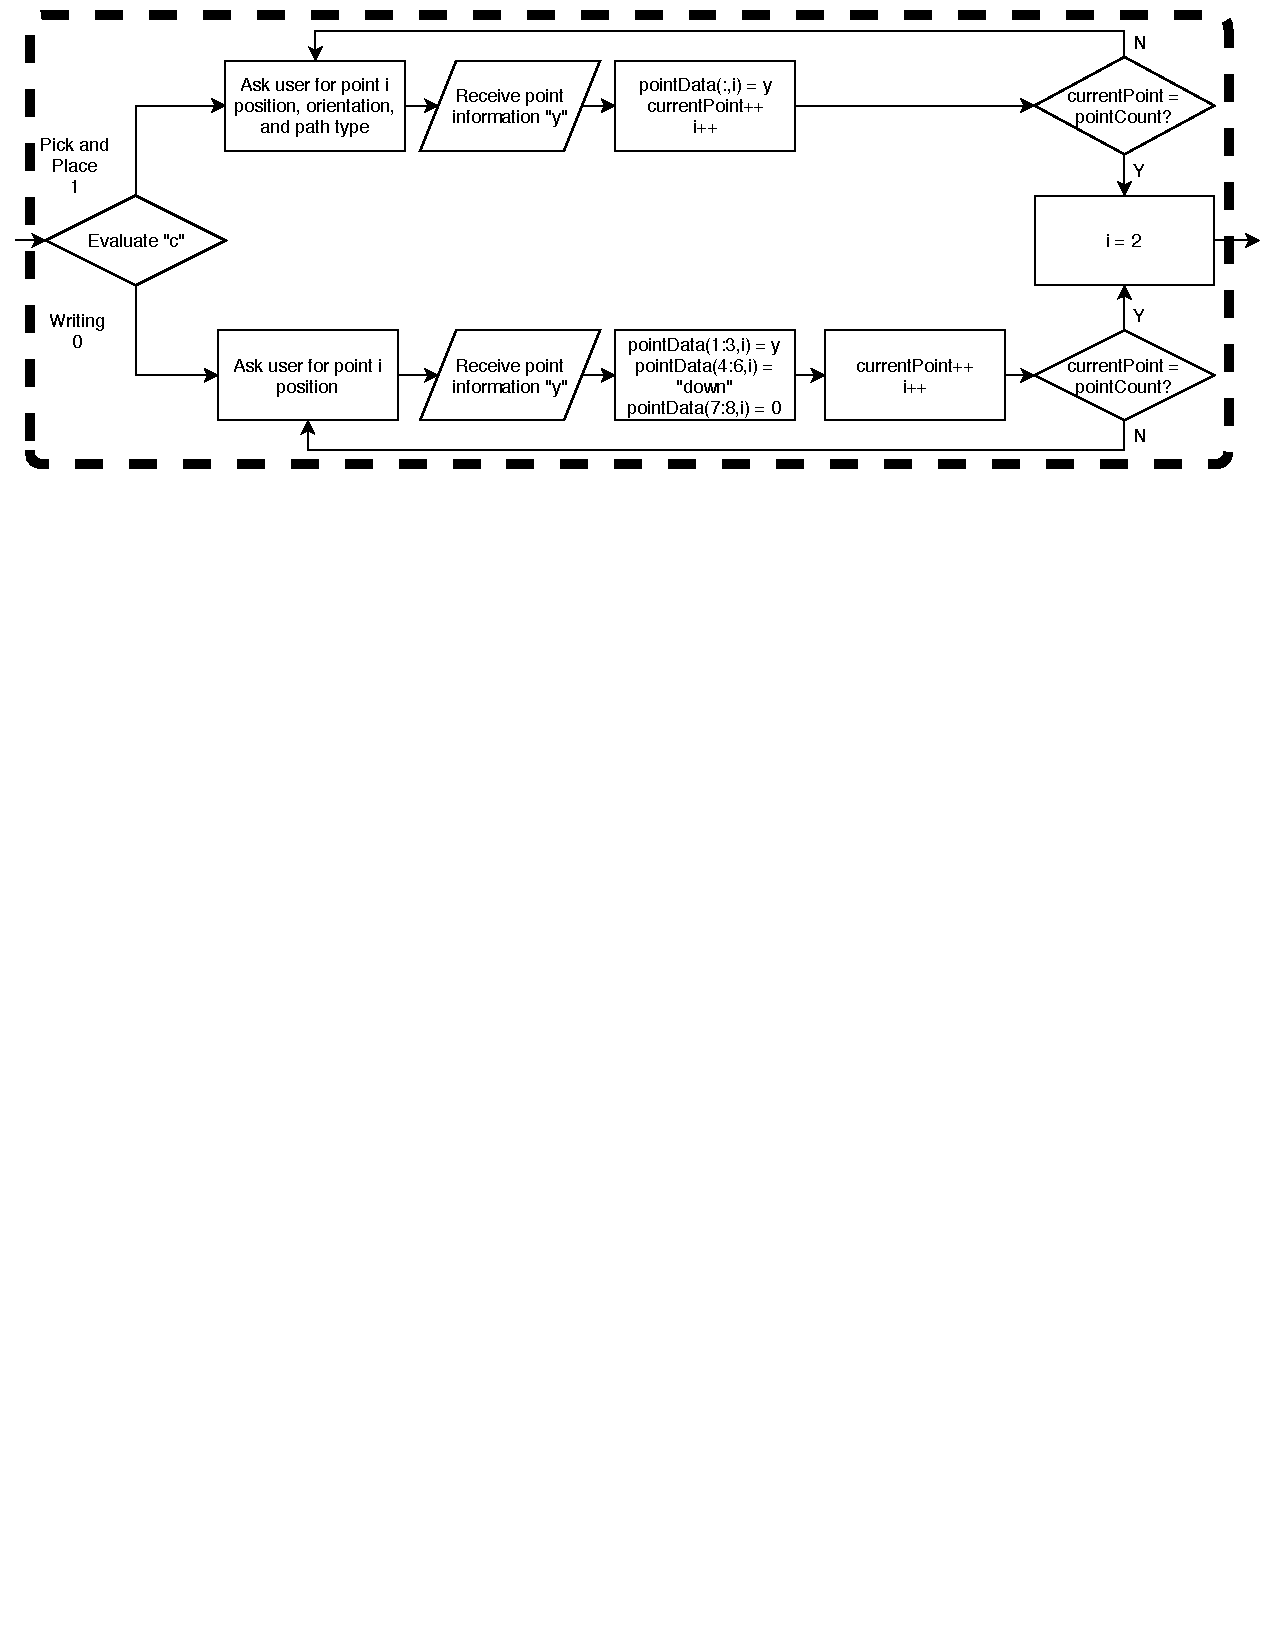
\includegraphics[width=\textwidth]{sf2}
  \caption{Software Flowchart Subsection 2}
  \label{fig:sf2}
\end{subfigure}
\end{figure}

\emph{Figure \ref{fig:sf2}} shows that the path type variable ‘c’ is used to determine what information is necessary to collect. If the user is doing a writing task, the software only collects the x, y, and z distances for the point and assumes that the end effector orientation will be facing down so that the marker is vertical. If the user is doing pick and place, the software prompts the user for the x, y, z, phi, theta, psi, path type, and end effector data. The software loops until all the points have been input.

The next block in the software flowchart calculates the total points necessary to complete the task. The overview for this section can be seen in \emph{Figure \ref{fig:sf3}}.

\begin{figure}[htp]\ContinuedFloat
  \begin{subfigure}[c]{\textwidth}
  \center
  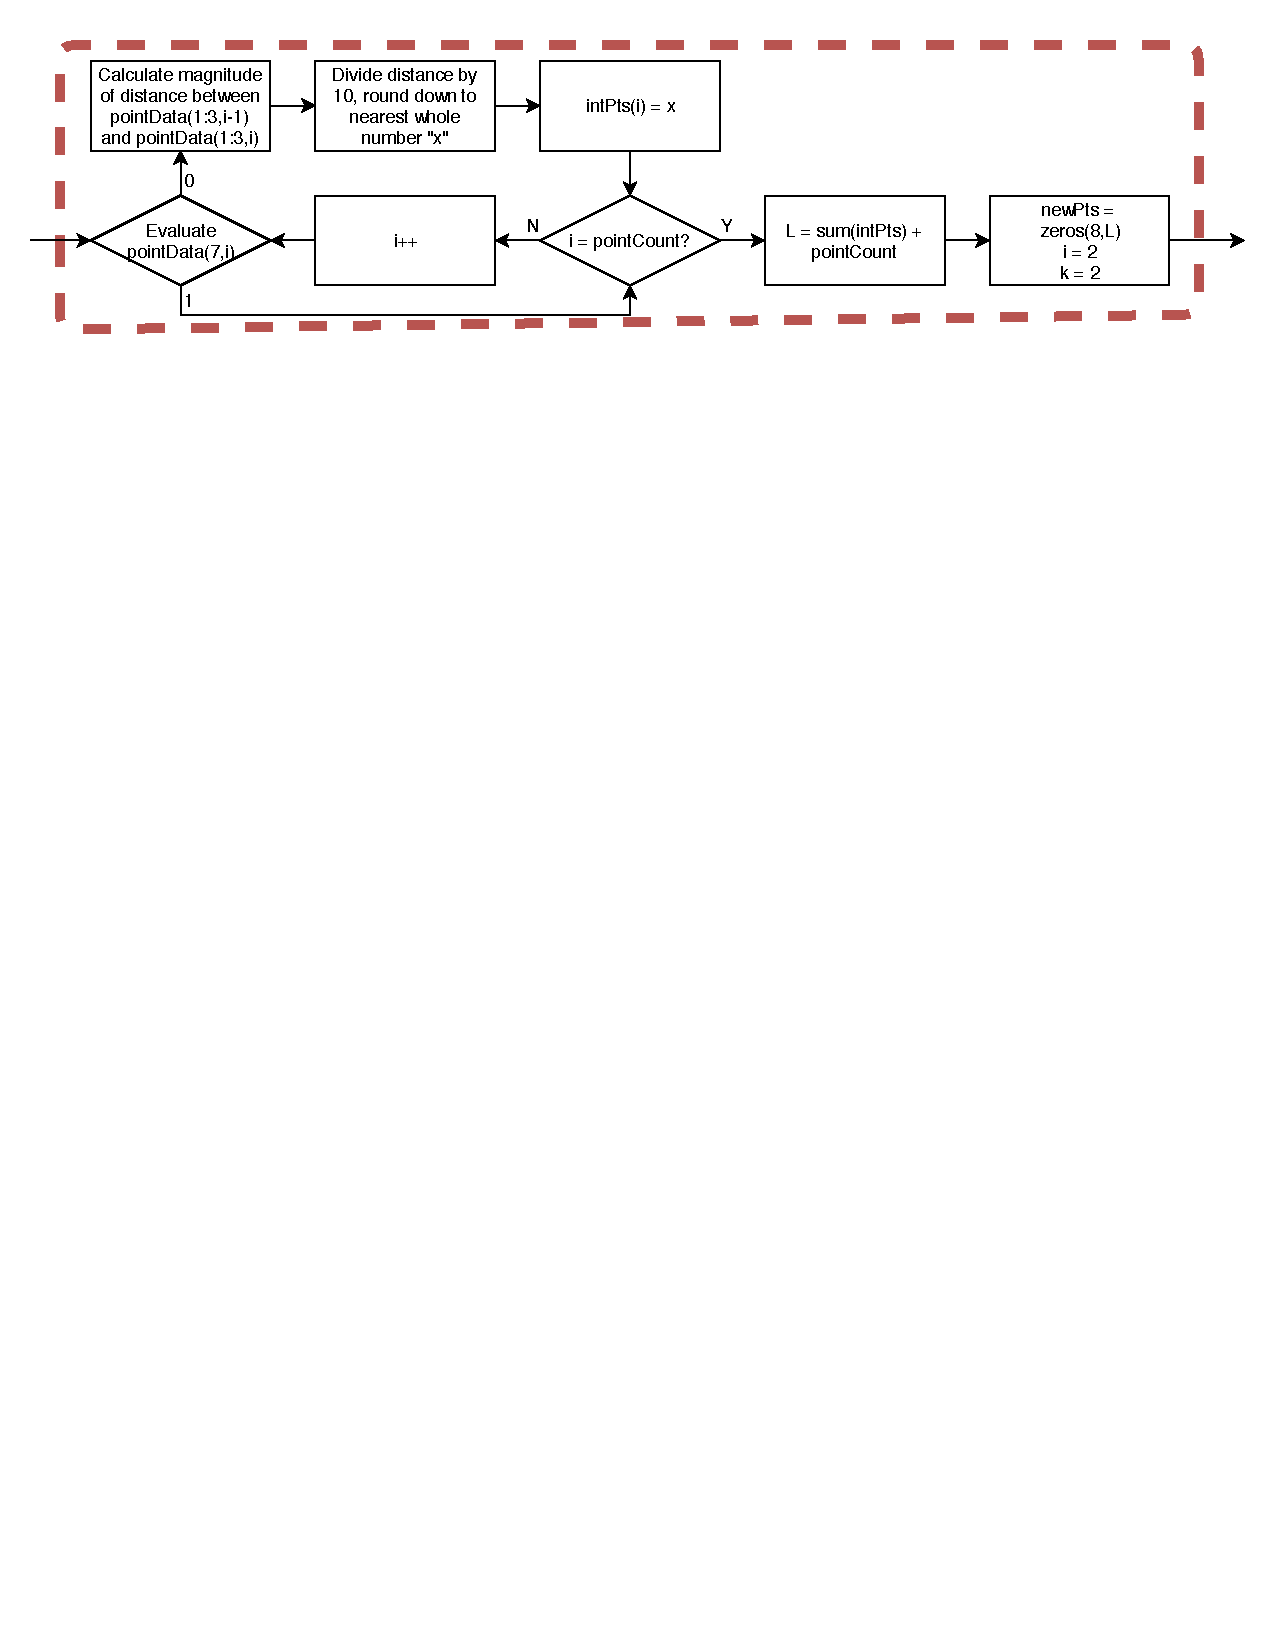
\includegraphics[width=\textwidth]{sf3}
  \caption{Software Flowchart Subsection 3}
  \label{fig:sf3}
  \end{subfigure}
\end{figure}

As seen in \emph{Figure \ref{fig:sf3}}, the section of software calculates the distance between the current point and the previous point if the path type is cartesian straight line and divides the distance by ten to find the number of centimeters between the two points. This value is stored as the necessary number of intermediate points, and the software will loop through until every point has been checked. The section of code also stores the total number of points that will be used as the variable level for later use.

The fourth code block in the flowchart creates and stores the necessary intermediate points along the desired path, shown in \emph{Figure \ref{fig:sf4}}.

\begin{figure}[htp] \ContinuedFloat
  \begin{subfigure}[c]{\textwidth}
  \center
  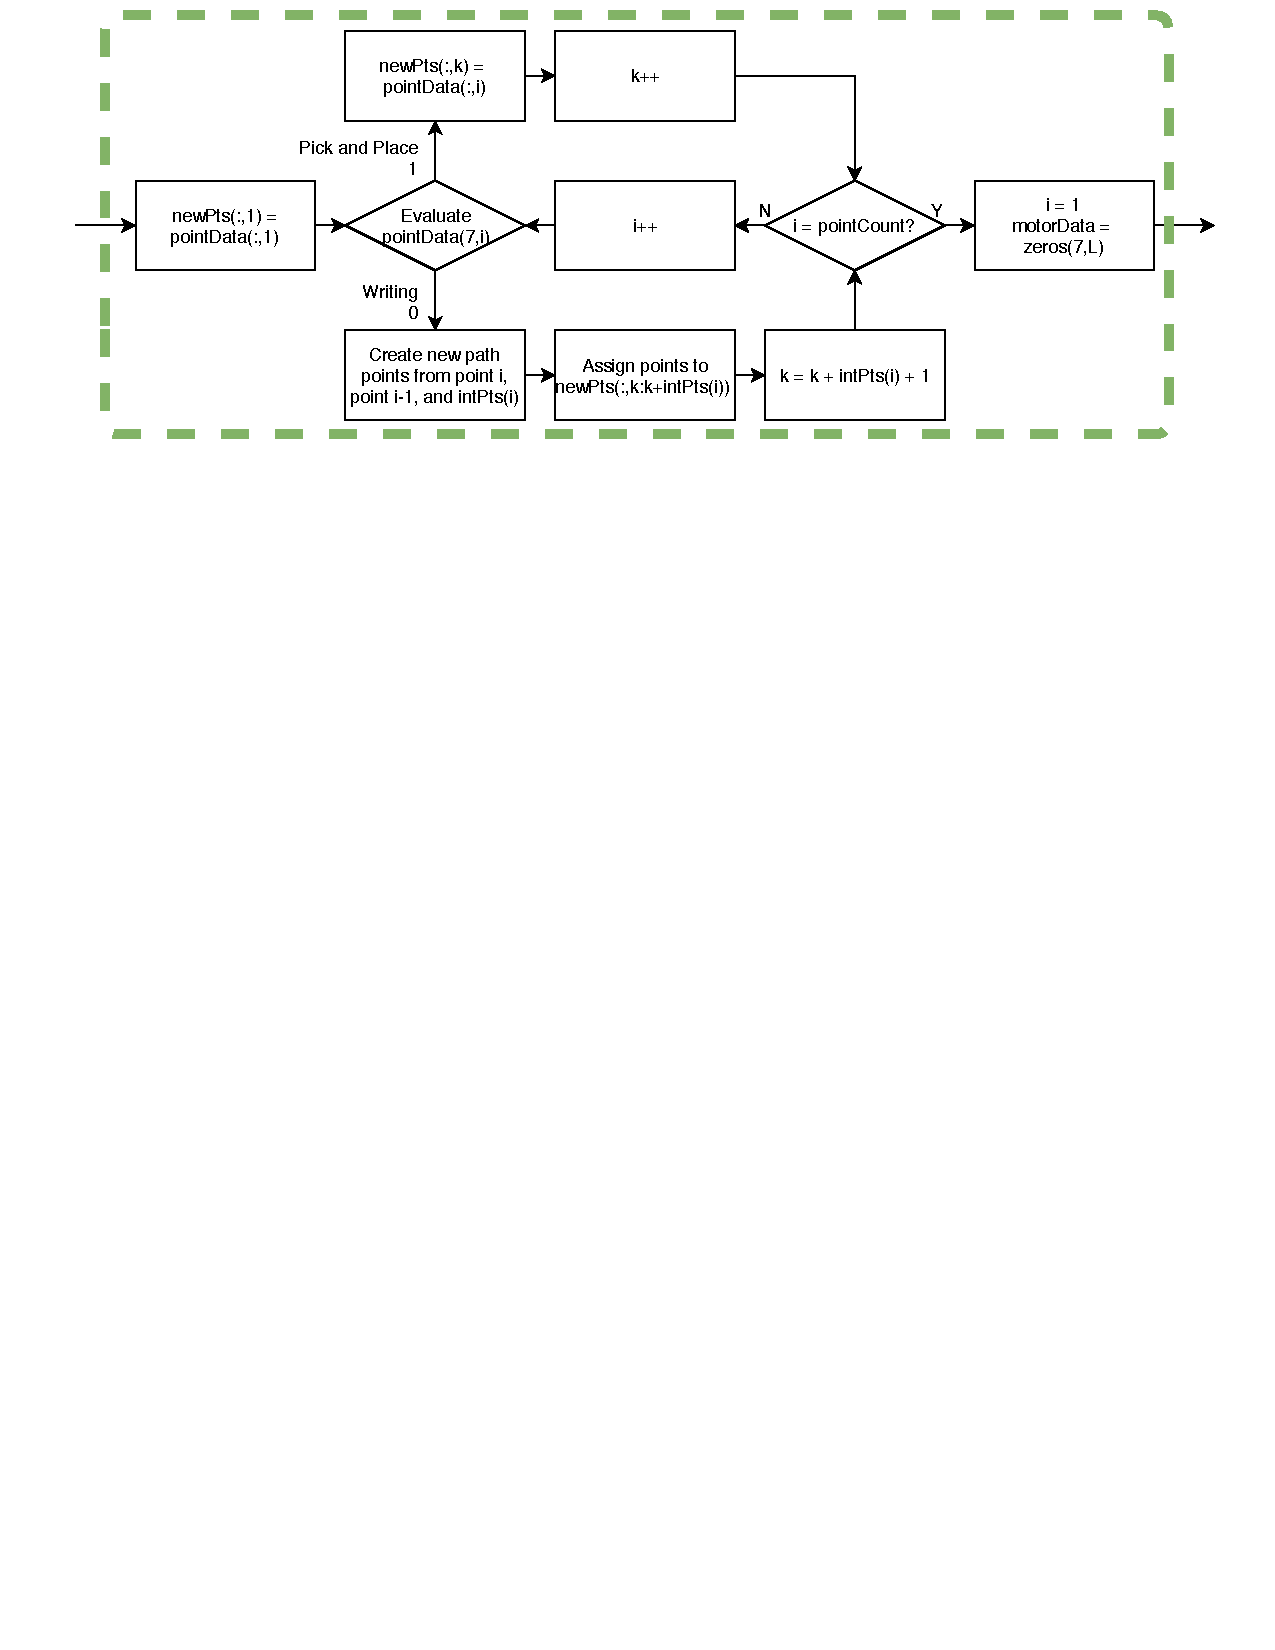
\includegraphics[width=.99\textwidth]{sf4}
  \caption{Software Flowchart Subsection 4}
  \label{fig:sf4}
  \end{subfigure}
\end{figure}
\looseness=-1

The code shown in \emph{Figure \ref{fig:sf4}} creates points every centimeter if the path type is cartesian straight line using the number of path points stored for each point from the previous block of software. This ensures that a straight line will be followed between the two user input points. If the path type is a straight line in the joint space, the software does not add any intermediate points since the path seen in the cartesian space does not matter.

The fifth code block in the flowchart calculates inverse kinematics of the points defined in the previous block of code and stores the angles as counts that can be used by the servos. The overview of this section can be seen in \emph{Figure \ref{fig:sf5}}.

\begin{figure}[htp] \ContinuedFloat
  \begin{subfigure}[c]{\textwidth}
  \center
  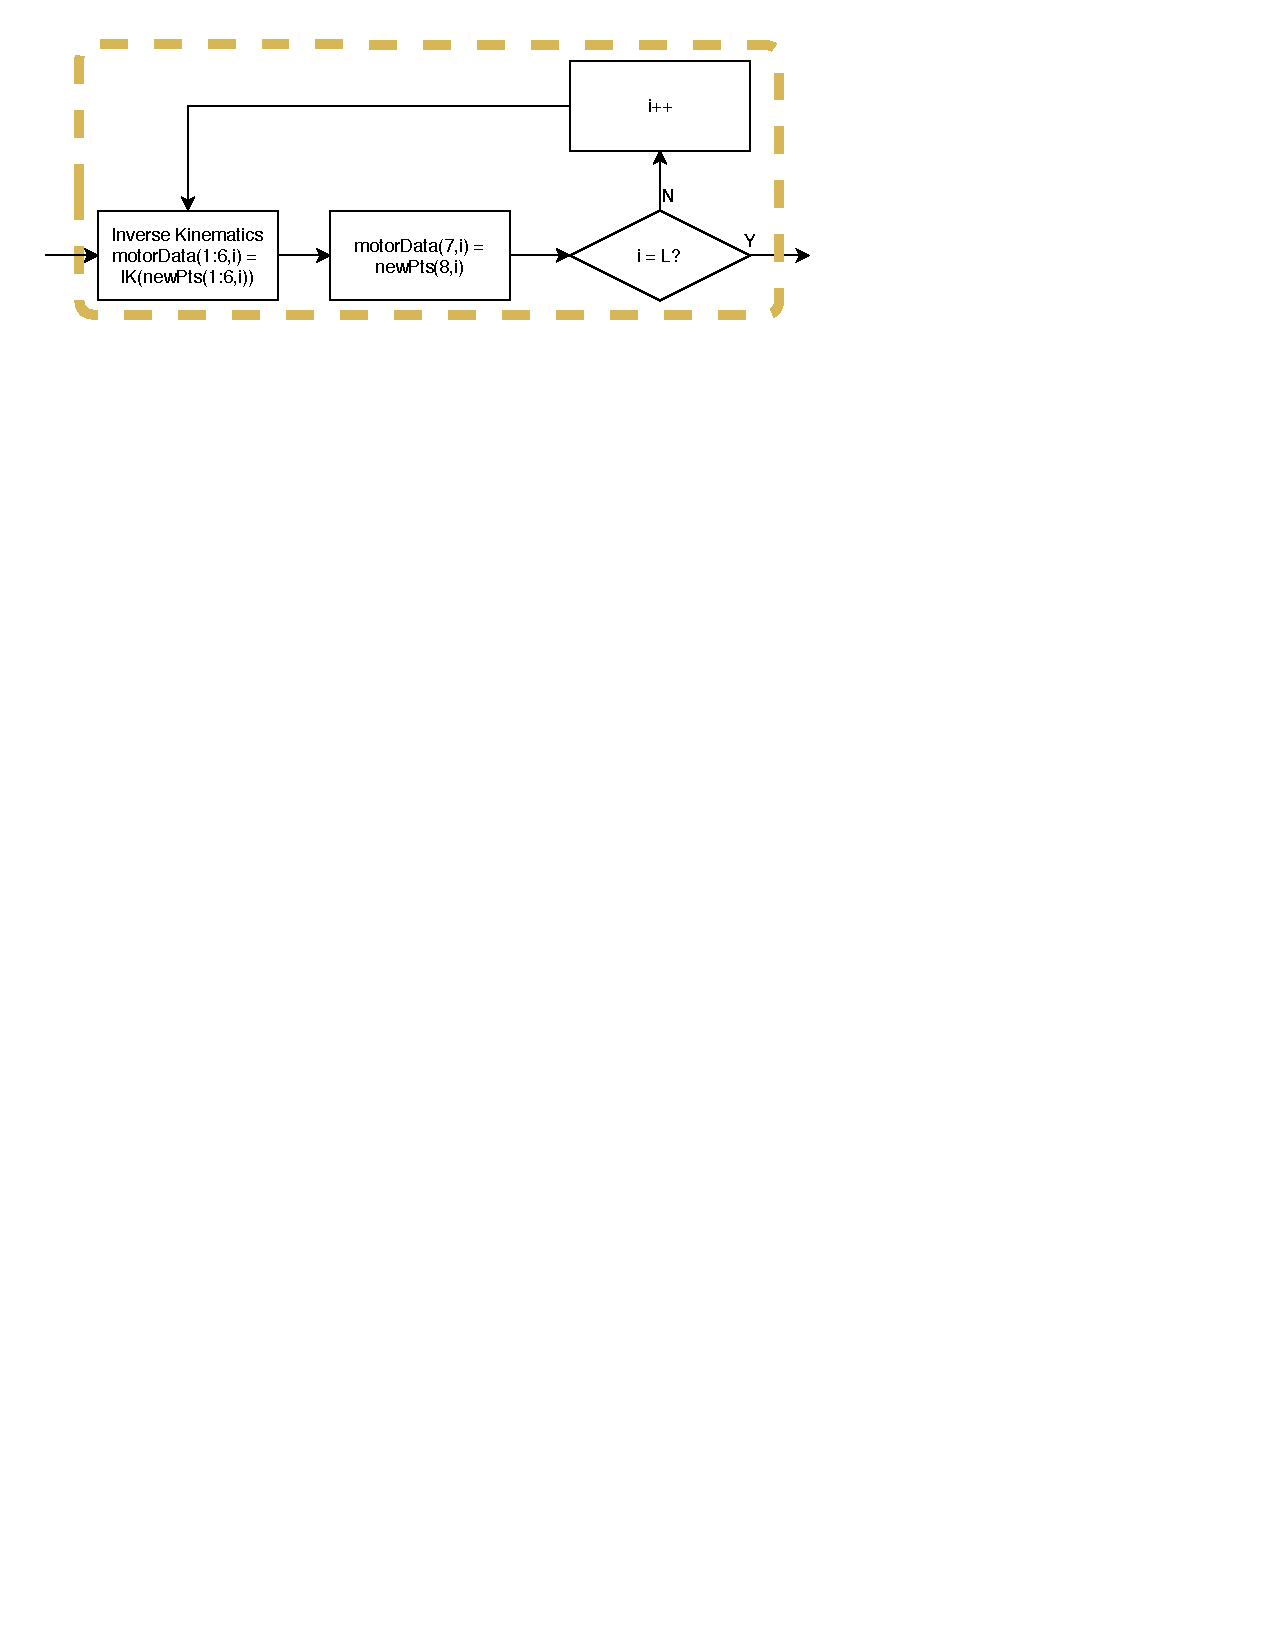
\includegraphics[width=\textwidth]{sf5}
  \caption{Software Flowchart Subsection 5}
  \label{fig:sf5}
  \end{subfigure}
\end{figure}

\emph{Figure \ref{fig:sf5}} shows that the new points found in the prior section of code are run through an inverse kinematics function that will output the necessary counts the servos can utilize. The code iterates through each point until the inverse kinematics have been calculated for all points.

The final block in the software diagram runs the manipulator through the desired task, with this section of code requiring user input at certain stages depending on the path type, seen in \emph{Figure \ref{fig:sf6}}.
\begin{figure}[htp] \ContinuedFloat
  \begin{subfigure}[c]{\textwidth}
  \center
  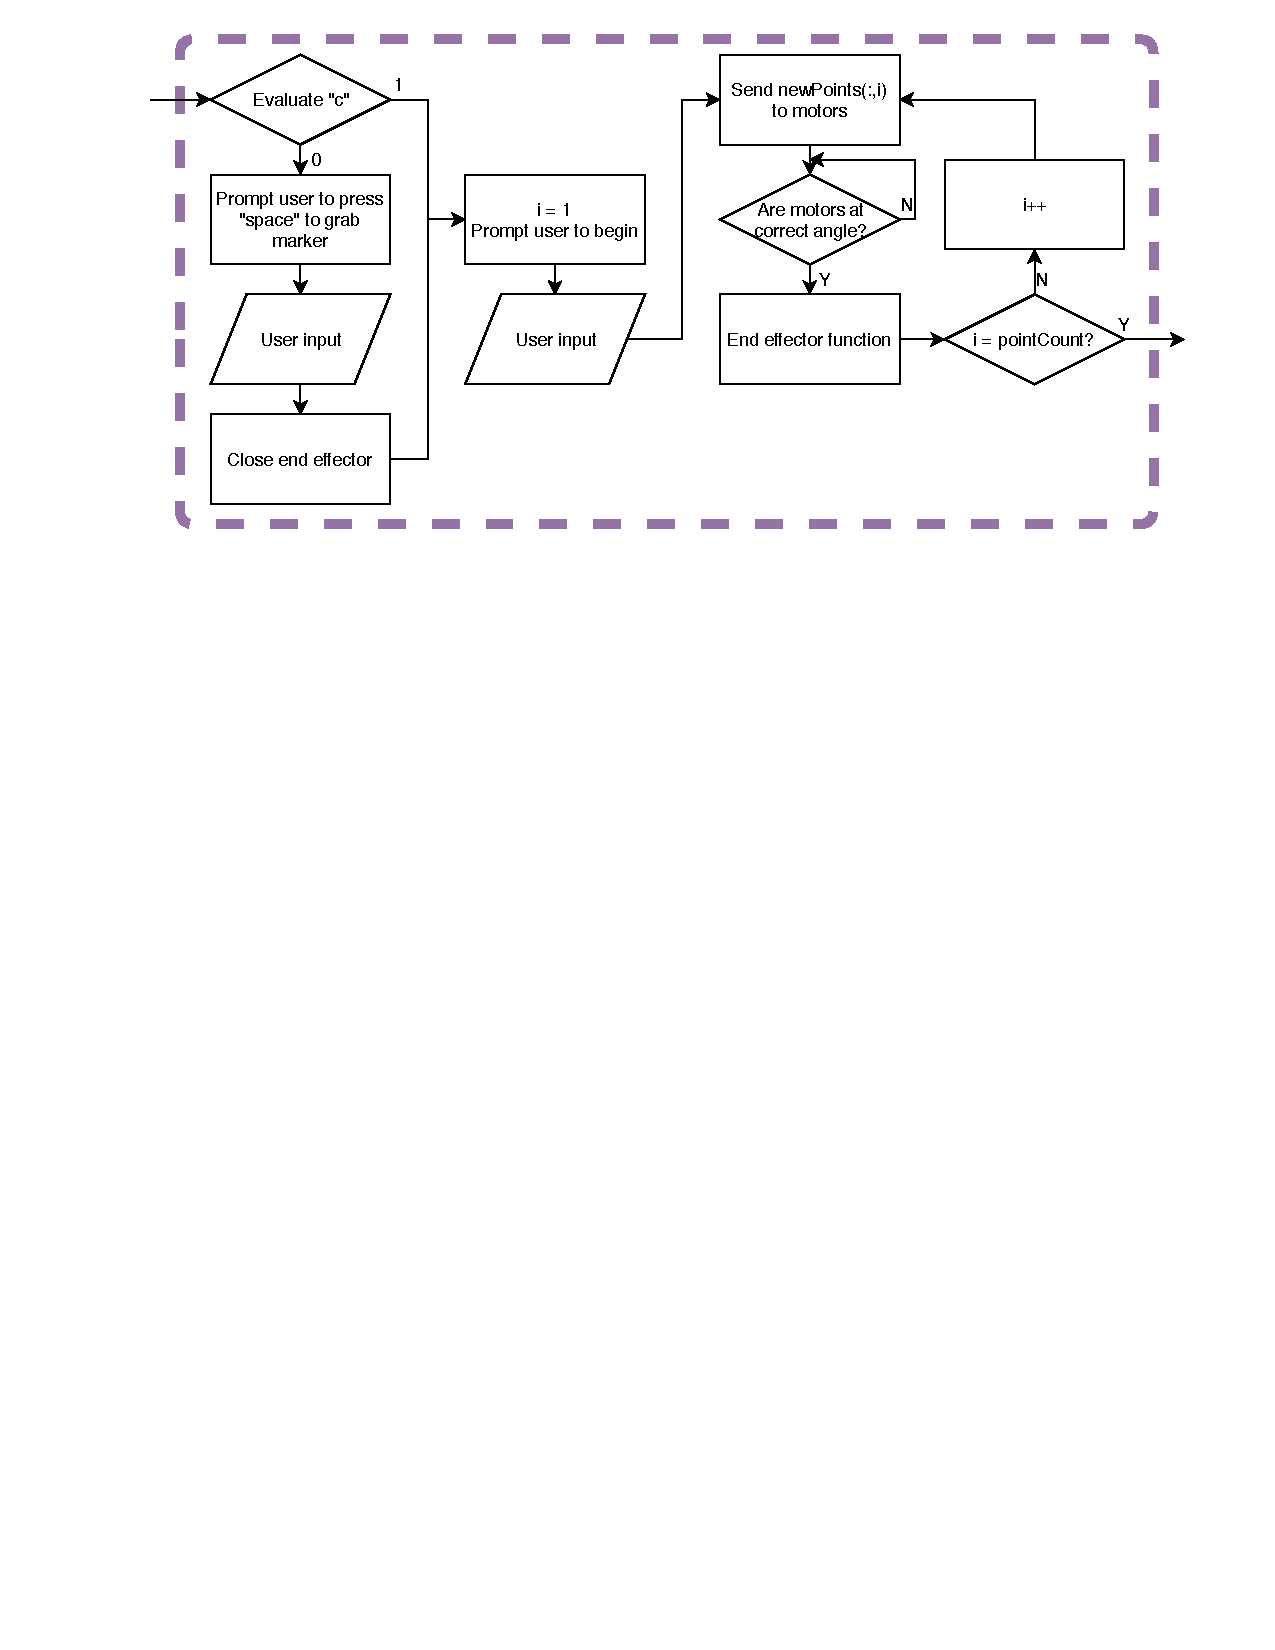
\includegraphics[width=\textwidth]{sf6}
  \caption{Software Flowchart Subsection 6}
  \label{fig:sf6}
  \end{subfigure}
\end{figure}

The code in \emph{Figure \ref{fig:sf6}} prompts the user to press space to close the end effector and grab the marker if drawing was the specified task, otherwise the software jumps straight into prompting the user to begin the task, and when the user begins the task the counts for each position are sent to the servos one at a time. The counts for the next position are not sent to the servos until the servos have reached the desired positions and the end effector function has been completed if there is one.

% 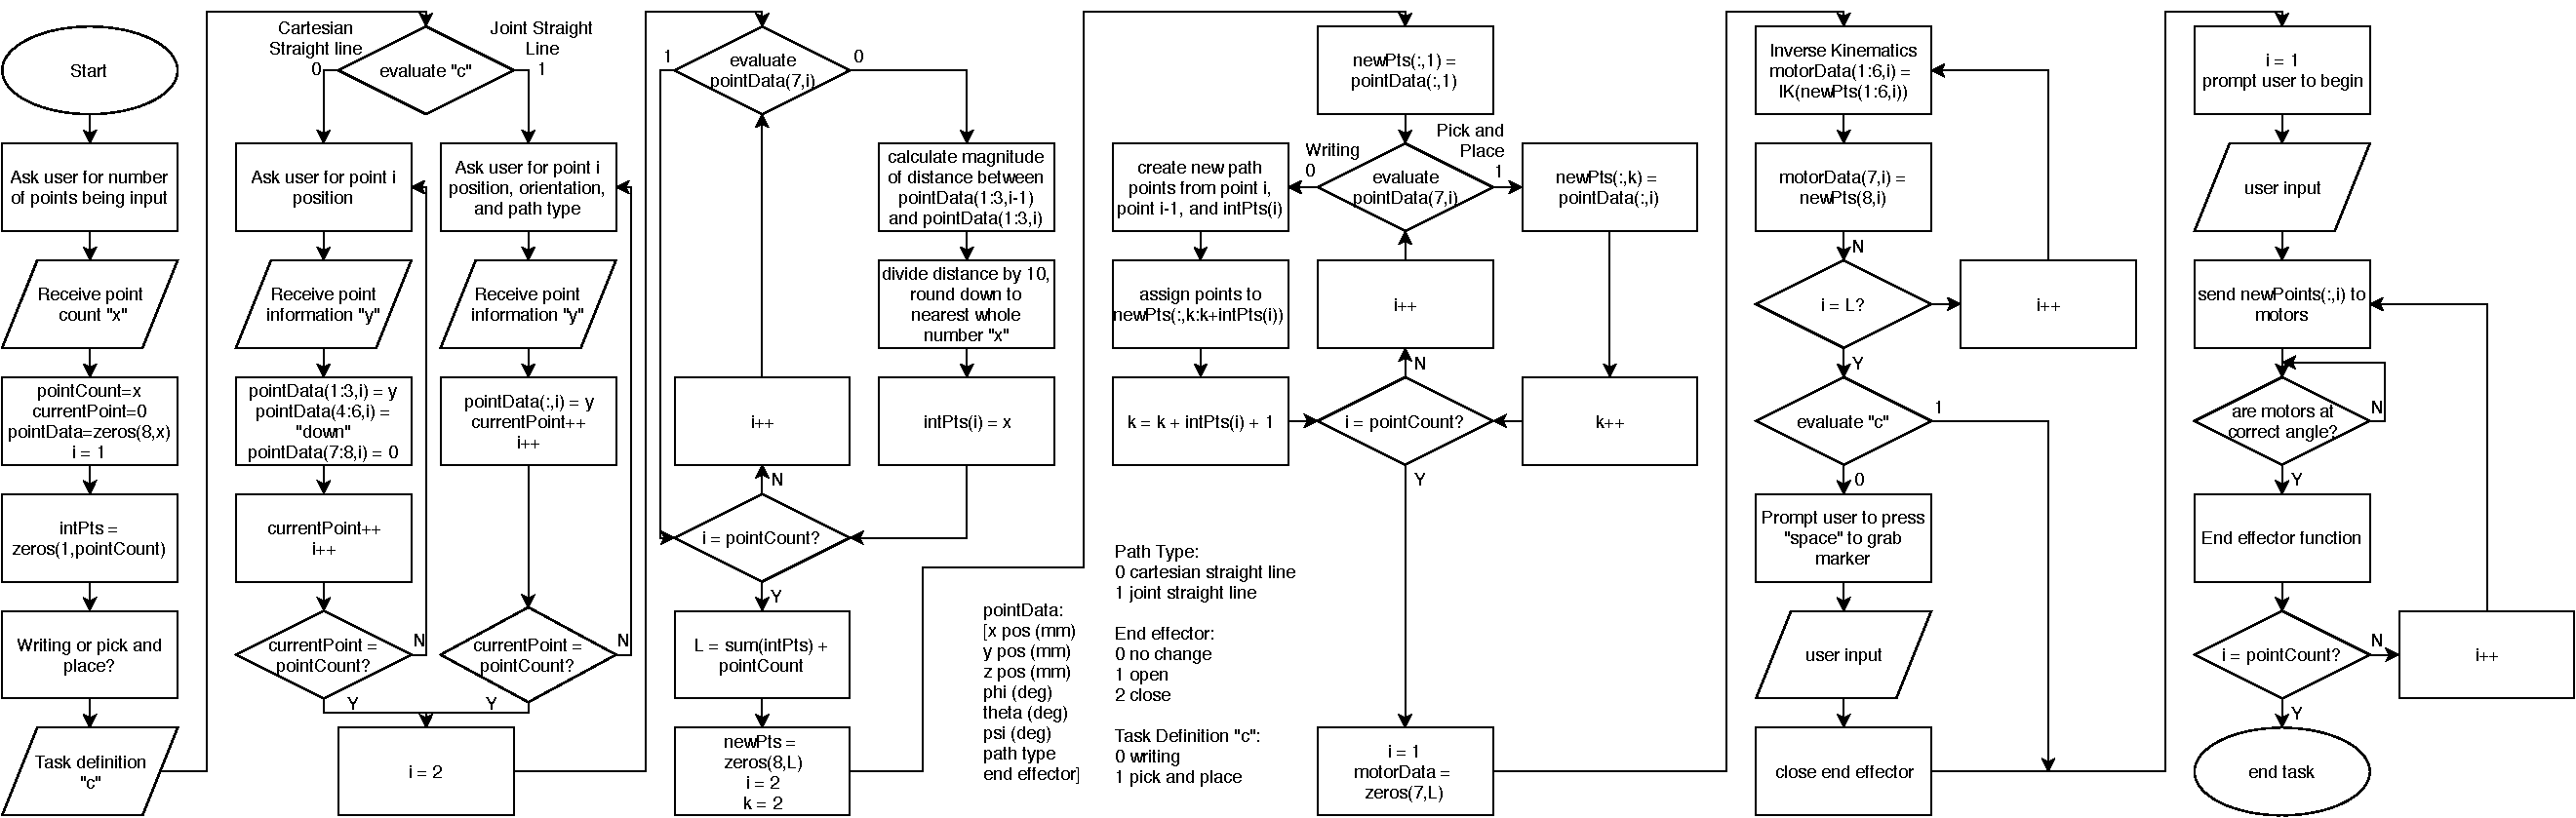
\includepdf[landscape,pages=-]{sflow}
\newpage
\subsection{Project Status and Future}
\begin{itemize}[label=---]
  \item Print Differential
  \item Cut Aluminum Supports
  \item Print Base
  \item Print Link 1
  \item Test Link 1 and Differential
  \item Print Differential Support
  \item Test Differential
  \item Test Link 1 Pulleys
  \item Test Link 1 with Motors
  \item Test Motor Control of Differential
  \item Test Link 1 With Load
  \item Implement Kinematics in Python
  \item Test Kinemtics with Motors
\end{itemize}
% The Gantt chart can be seen on the following page.
% 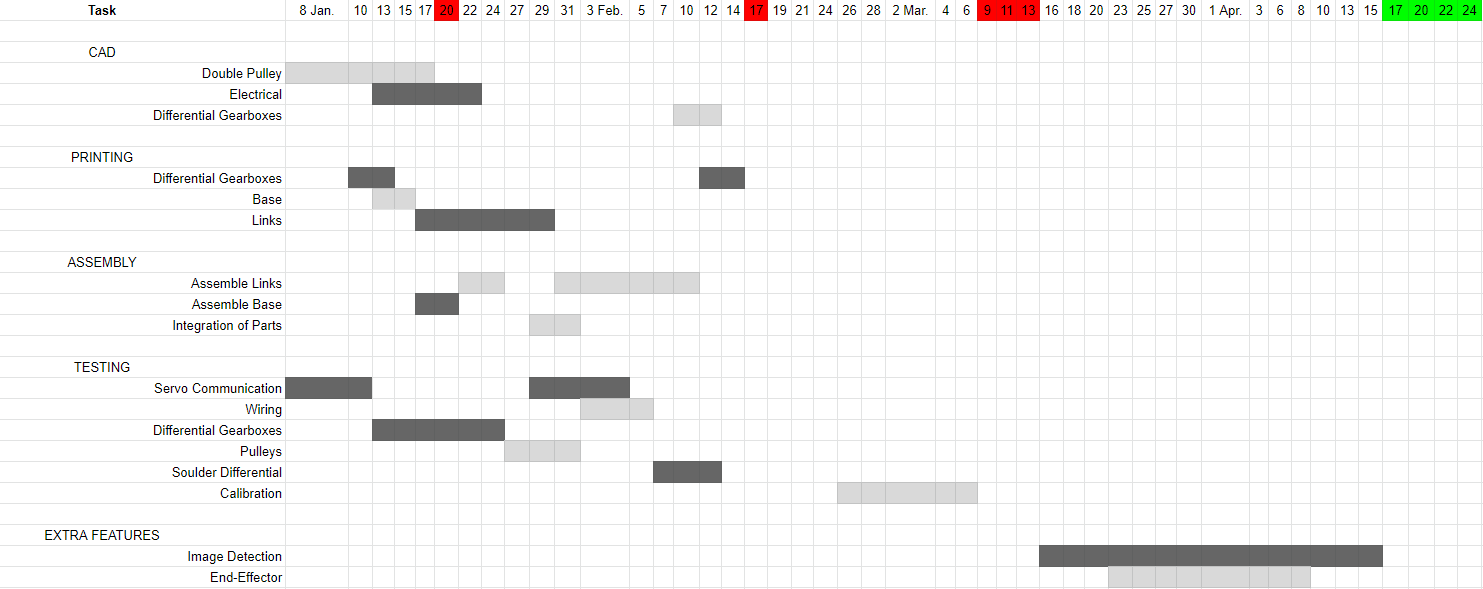
\includepdf[landscape,pages=-]{gantt}
\newpage
\subsection{Parts List}
\emph{Table \ref{tab:bom1}} lists the parts MEIOSIS will require to build the manipulator. The total cost is \$629.22 including shipping. Specification 1.1b required MEIOSOS’s cost to develop the manipulator be less than \$800. In addition to pulley belts for the current configuration, \emph{Table \ref{tab:bom1}} allocates \$20 for two additional belt sizes to increase joint 1/2’s and joint 3’s torque by a factor of 10. One belt size and the belt must be purchased in packs of 3 from Automation Direct. \emph{Table \ref{tab:bom1}}  accounts for increased cable lengths of 500 mm to communication bus signals from motor 2 to 3 and motor 3 to 4 and 350 mm to communication bus signals from motor 5 to 6. Motors are identified in [ZACK’S FIGURE]. Aside from electronic hardware, Figure ZZ accounts for physical hardware: To 100 threaded press-fit inserts. The manipulator will require between 21 and 46 inserts. The majority of inserts attach MX-12W servos to the manipulator. Mounting hardware accompanies each servo.
%TODO: [ZACK’S FIGURE] ^

\renewcommand{\arraystretch}{1.25}
\begin{table}[htp]
  \center
  \caption{MEIOSIS Bill of Materials with Costs}
  \label{tab:bom1}
\begin{tabular}{cC{3cm}@{\hskip 3pt}c@{\hskip 3pt}C{3cm}@{\hskip 3pt}|C{3cm}}
\multirow{2}{*}{\textbf{Part}} & \multirow{2}{*}{\textbf{Retailer}} & \multirow{2}{*}{\textbf{Quantity}} & \textbf{Unit Cost (USD)} & \textbf{Total Cost (USD)} \\\hline
3 pack, 300 tooth & \multirow{4}{*}{\shortstack[c]{Automation \\Direct}} & 1 & 11.5 & 11.5 \\
3 pack, 208 tooth &  & 1 & 9.5 & 28.5 \\
Base second belts &   & 1 & 10 & 10 \\
Link 3 second belts & & 1 & 10 & 10 \\\arrayrulecolor{gray}\hline
MX-12W & \multirow{4}{*}{\shortstack[c]{Trossen \\Robotics}} & 6 & 65.9 & 395.4 \\
500 mm, 1/2 pulleys &  & 2 & 3.95 & 7.9 \\
350 mm, 3 pulley &  & 1 & 2.95 & 2.95 \\
EE &  & 1 & 24.95 & 24.95 \\\arrayrulecolor{gray}\hline
Pi 3 B & \multirow{2}{*}{Amazon} & 1 & 37.99 & 37.99 \\
Bearings &  & 1 & 8.99 & 8.99 \\\arrayrulecolor{gray}\hline
\multirow{2}{*}{2 Sch 10 12" Al tube} & Industrial Metal Sales & 1 & 2.99 & 2.99 \\\arrayrulecolor{gray}\hline
\multirow{2}{*}{12 V, 5 V power supply} & Digi-Key Electronics & 1 & 43.21 & 43.21 \\\arrayrulecolor{gray}\hline
Automation Direct & \multirow{5}{*}{Shipping} & \multirow{5}{*}{---} & \multirow{5}{*}{---} & 0 \\
Trossen Robotics &  &  & & 13.15 \\
Amazon & &  & & 0 \\
Industrial Metal Sales &  & &  & 26.36 \\
Digi-Key &  & &  & 8.99 \\
& & & \textbf{Total} & 629.22 \\
\end{tabular}
\end{table}

In addition to the costs listed in \emph{Table \ref{tab:bom1}}, \emph{Table \ref{tab:bom2}} shows all further costs for the end-user. Since the Embry-Riddle robotics lab has 3D printing available without affecting MEIOSIS’s \$800 budget, \emph{Table \ref{tab:bom2}} accounts for outsourced 3D printing costs sufficient to print the entire manipulator with six sets of pulleys. If the end-user owns a 3D printer, the 3D printing cost would effectively reduce to filament cost. Additionally, \emph{Table \ref{tab:bom2}} assumes the end-user does not already possess an AX-12A servo to be used with the end-effector. Further, \emph{Table \ref{tab:bom2}} assumes the manipulator would be more accessible to end-users by using a proprietary U2D2 communication module in lieu of a soldered or bread-board circuit. The robotics lab has an AX-12A servo and U2D2 communication module MEIOSIS will use. With the aforementioned additional costs, the MEIOSIS manipulator costs the end-user \$1,007.98 including shipping costs. While \$1,007.98 is slightly above the maximum cost of \$1000 from specification 1.1a, it provides greater accessibility, which may be diminished by assuming end-users posess 3D printers.

\renewcommand{\arraystretch}{1.25}
\begin{table}[htp]
  \center
  \caption{End-User Bill of Materials with Costs}
  \label{tab:bom2}
  \begin{tabular}{C{3cm}C{3cm}@{\hskip 3pt}c@{\hskip 3pt}C{3cm}@{\hskip 3pt}|C{3cm}}
  \multirow{2}{*}{\textbf{Part}} & \multirow{2}{*}{\textbf{Retailer}} & \multirow{2}{*}{\textbf{Quantity}} & \textbf{Unit Cost (USD)} & \textbf{Total Cost (USD)} \\\hline
  Aforementioned Costs & \multirow{2}{*}{\emph{Table \ref{tab:bom1}}} & \multirow{2}{*}{---} & \multirow{2}{*}{---} & 629.22 \\
  \multirow{2}{*}{U2D2} & Trossen Robotics & \multirow{2}{*}{1} & \multirow{2}{*}{49.9} & \multirow{2}{*}{49.9}\\
  \multirow{2}{*}{EE with servo} & Trossen Robotics & \multirow{2}{*}{1} & \multirow{2}{*}{64.95} & \multirow{2}{*}{64.95} \\
  3D PLA outsourcing (incl. shipping) & \multirow{2}{*}{Craft Cloud} & \multirow{2}{*}{1} & \multirow{2}{*}{288.86} & \multirow{2}{*}{288.86} \\
  & & & \textbf{Total} & 1007.98 \\
  \end{tabular}
\end{table}
\renewcommand{\arraystretch}{1}
% \begin{enumerate}[label=\alph*.]
%   \item Description for callout a
%   \item Description for callout b
% \end{enumerate}

% Example citations:
% \cite{DBLP:journals/corr/JohnsonAL16}
% \cite{DBLP:journals/corr/abs-1803-09820}
% \cite{DBLP:journals/corr/RonnebergerFB15}


\newpage
\section*{Acknowledgements \& Attributions}
We would like to acknowledge the following people for their contibutions in creating this report.
\begin{itemize}
  \item Dr. Isenberg
  \item Dr. Schipper
\end{itemize}

\nocite{*}
\bibliographystyle{plainnat}
\raggedright
\bibliography{bibs}

\newpage
\appendix
\renewcommand\thesection{\Roman{section}}
\renewcommand\thesubsection{\roman{subsection}}
\hiddenappsec{Appendix}\label{sec:app}
% \section{Appendix}\label{sec:app}
\hiddenappsub{Relevant Figures and Materials}
% \subsection{Relevant Figures and Materials}
\begin{figure}[htp]
  \centering
  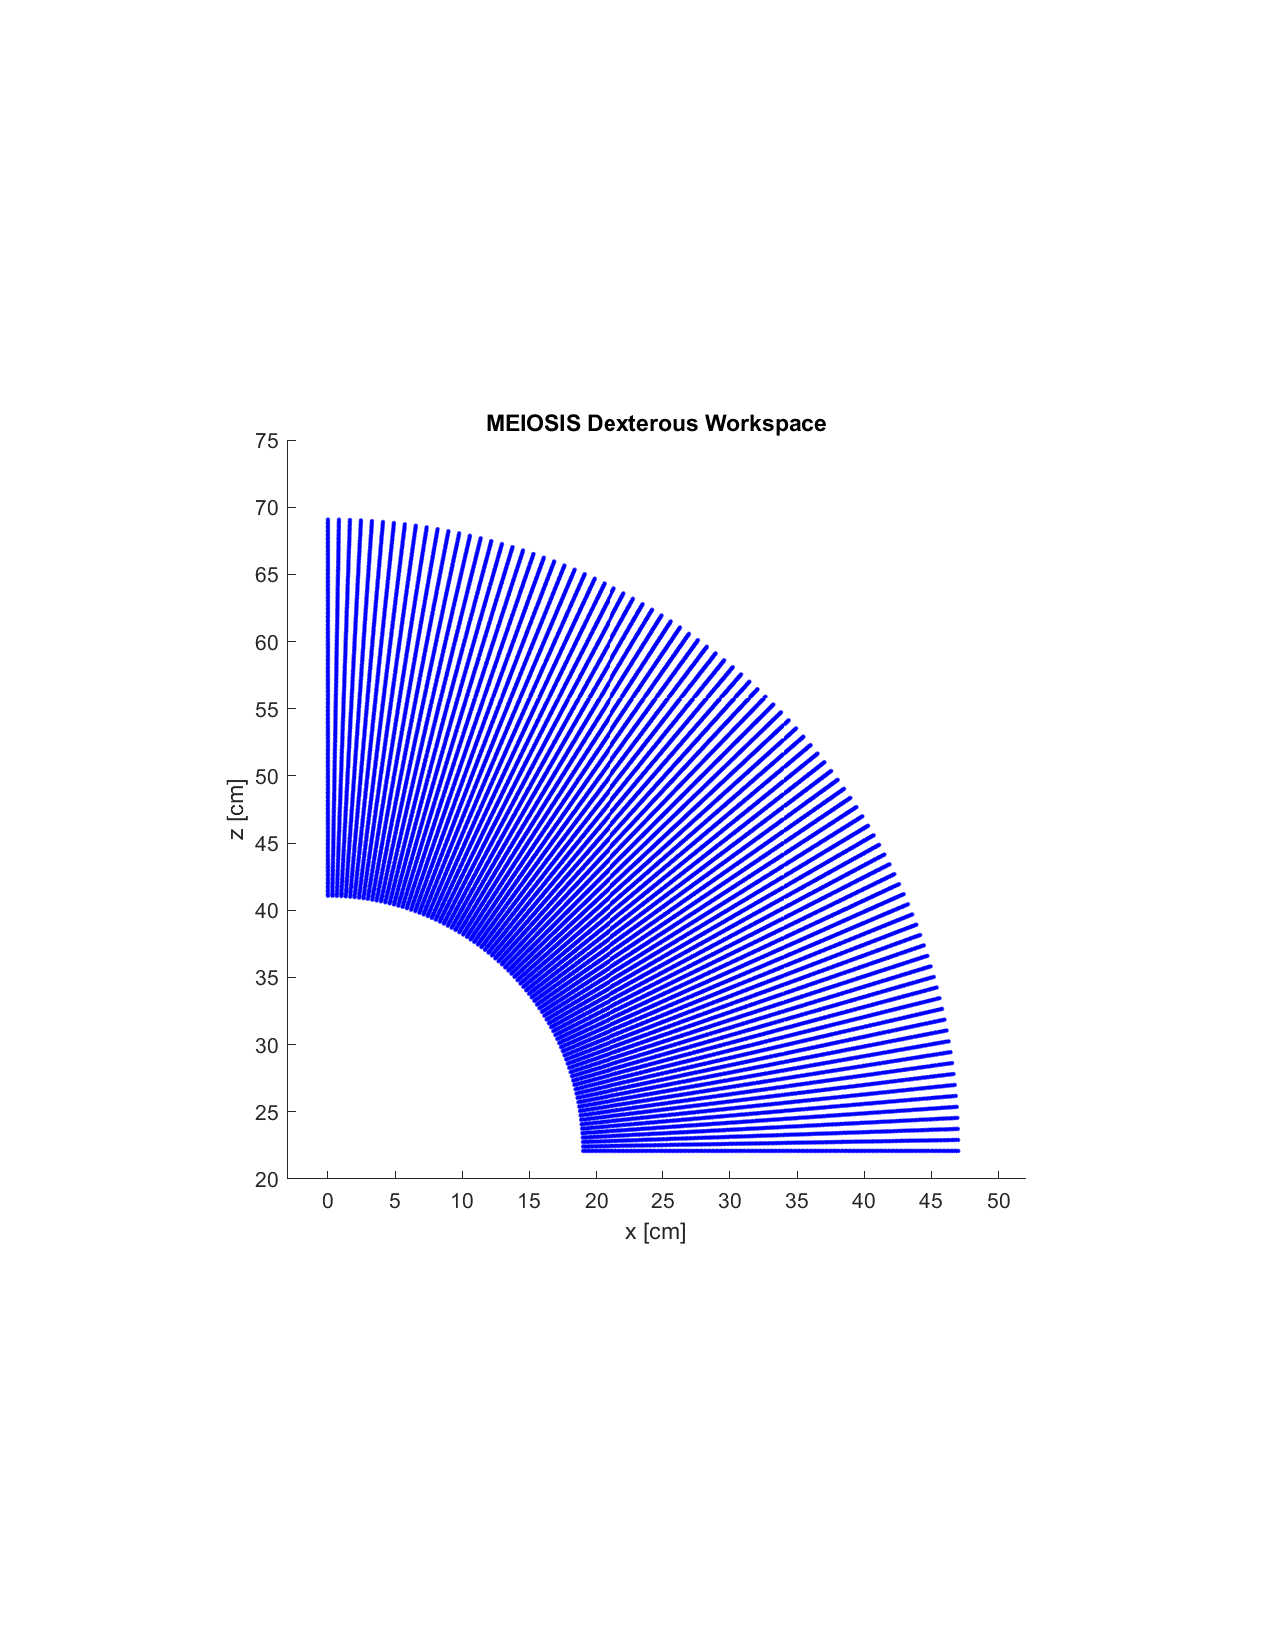
\includegraphics[frame,width=.75\textwidth]{dex}
  \caption{Cross Section of Dexterous Workspace Quadrant}
  \label{fig:dex}
\end{figure}
\hiddenappsub{CAD Drawings}
% \subsection{CAD Drawings}
The complete drawing package is attached.
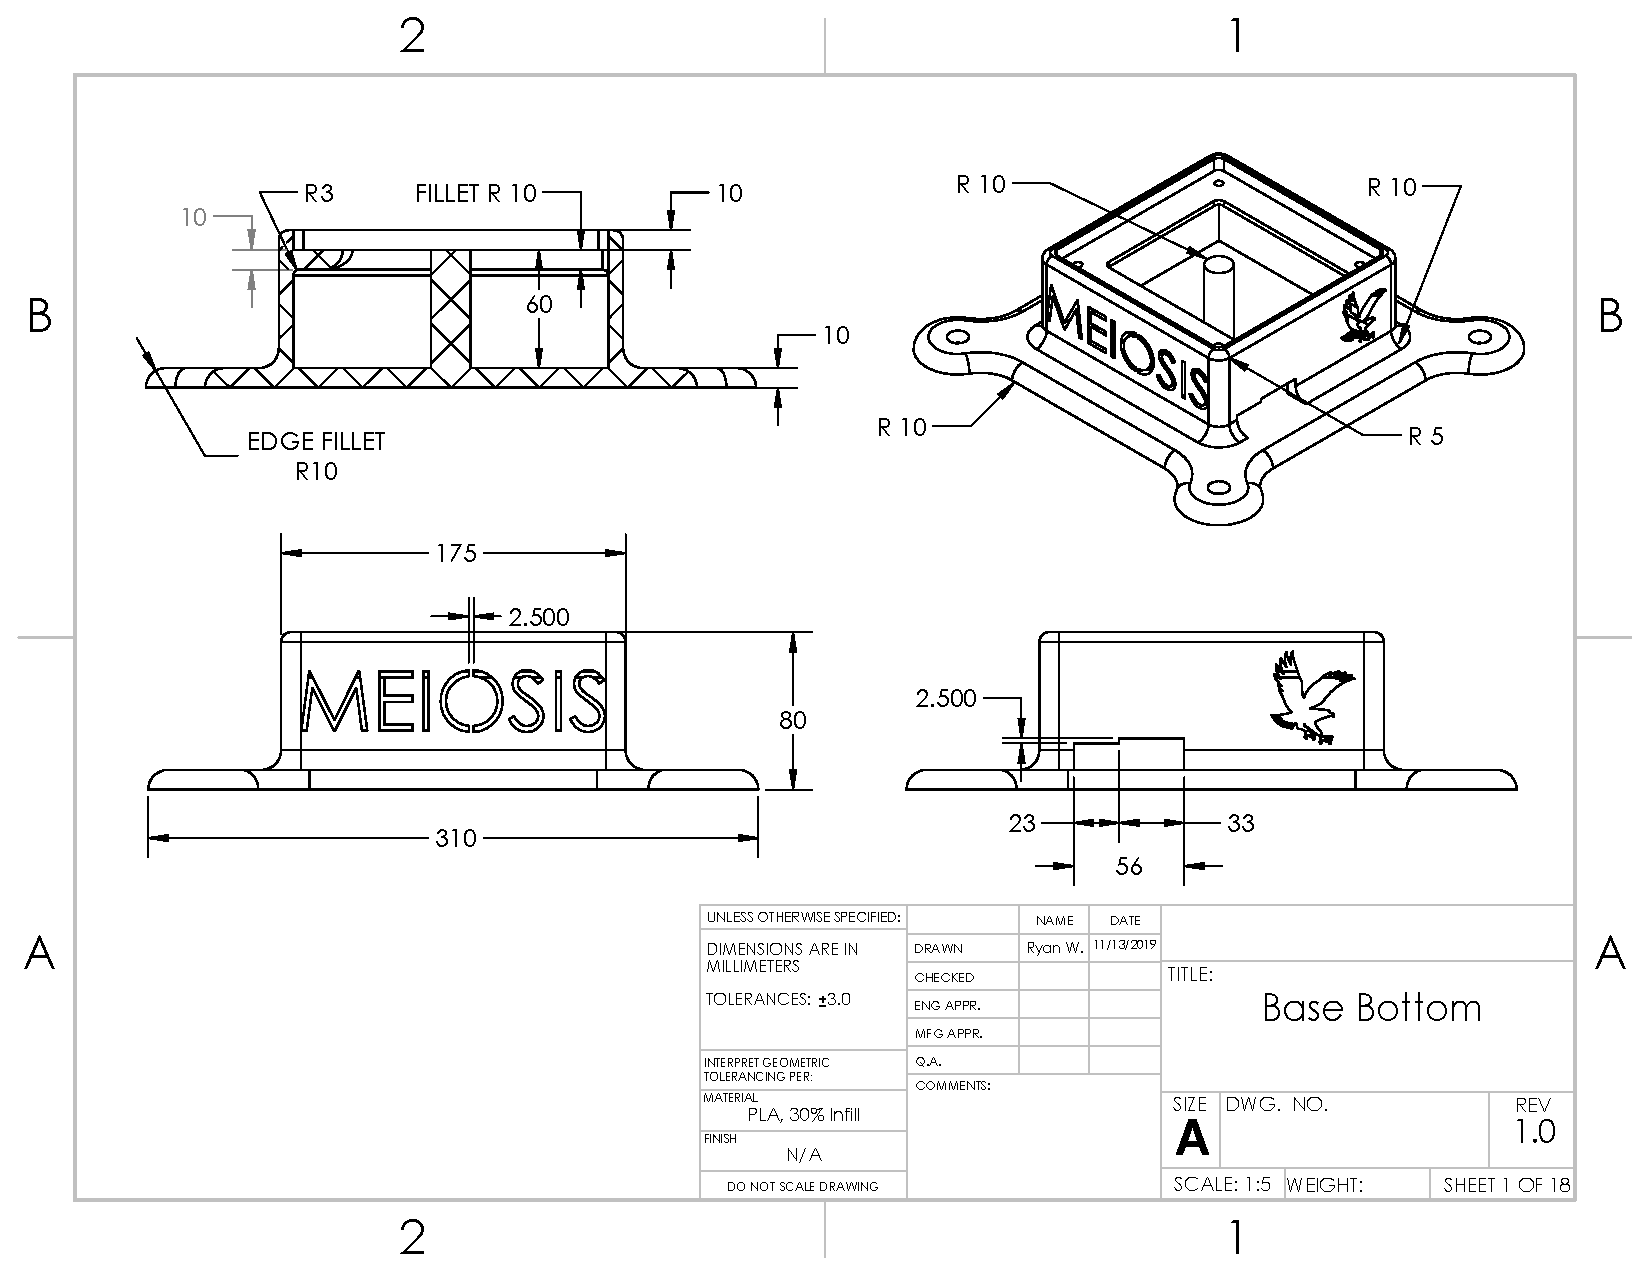
\includepdf[landscape,pages=-]{drawings}
\hiddenappsub{Salient Code}
% \subsection{Salient Code}
\begin{lstlisting}[frame=lines,style=Matlab-editor,basicstyle = \mlttfamily, label=code:mmodel, caption=Actuator Dynamics MATLAB Code]
% dynamixel motor model experiment
close all;clear;clc

% test loads mass moments of inertia
m = [.146 .088 0.108];          % mass (kg)
b = [.61277 .37227 0.28257];    % length (m)
h = [.01915 0.01915 0.0299];    % height (m)
J = (1/12)*m.*(h.^2 + b.^2);

% path to csv files relative to script
datapath = 'data/AX12A/';
files = dir(strcat(datapath,'*.csv'));
numFiles = length(files);
% initialize variables
[damp, wn, Tp] = deal(zeros(numFiles,1));

for ii = 1:numFiles
    % load experimental data, skip 5 header lines
        M = csvread(strcat(datapath, files(ii).name),5,0);
    % clean data by removing outliers
        nani = (find(diff(M(:,1)) > 100));
        M(nani,:) = [];
    % show response
         figure();
         plot(M(:,1),M(:,2))
         title('Experimental Data')
    % find % OS
        peak = max(M(:,2));                        % peak value
        peaki = find(M(:,2)==peak, 1, 'first');    % peak value index
        ss = M(end,2);                             % steady state
        os = ((peak - ss) / ss) * 100;             % % OS
    % damping ratio
        damp(ii) = -log(os/100) / sqrt(pi^2 + log(os/100)^2);
    % find where the motor begins responding
        start = M(find(diff(M(:,2)) > 1, 1, 'first'), 1);
    % time to peak
        Tp(ii) = (M(peaki,1) - start) / 1000;
    % natural frequency
        wn(ii) = pi / (sqrt(1 - damp(ii)^2)*Tp(ii));
end

sol = zeros(4,1);
% no load case, 2*zeta*omega_n
sol(1) = 2*mean(damp(end-2:end))*mean(wn(end-2:end));
% no load case, omega_n^2
sol(2) = mean(wn(end-2:end))^2;

% obtain average damping ratio and natural frequencies for load cases
zeta = [mean(damp(1:3));mean(damp(4:6));mean(damp(7:9))];
omegan = [mean(wn(1:3));mean(wn(4:6));mean(wn(7:9))];

alpha = 2.*zeta.*omegan;
beta = omegan.^2;
A = zeros(3,2);
b = zeros(3,1);

for jj = 1:3
    A(jj,:) = [1, -(alpha(jj)*J(jj) + beta(jj)*J(jj))];
    b(jj) = alpha(jj) + beta(jj);
end

sol(3:4) = A \ b;
\end{lstlisting}

\vspace{10ex}

\begin{lstlisting}[frame=lines,style=Matlab-editor,basicstyle = \mlttfamily, caption=Forward Kinematics MATLAB Function]
function [r6,T6]= MeiosisFK(theta)

    %       Mapping between joint space and motor space
    N = 10;         %Gear Ratio
    A = [ 1/(2*N), 1/(2*N),   0, 0,   0,   0;
          1/(2*N),-1/(2*N),   0, 0,   0,   0;
                0,       0,-1/N, 0,   0,   0;
                0,       0,   0, 1,   0,   0;
                0,       0,   0, 0,-1/2, 1/2;
                0,       0,   0, 0, 1/2, 1/2];
    gamma = A*theta;

%     %Define Constants
%     LB = 12.275;
%     L1 = 0;
%     L2 = 25;
%     L3 = 20;
%     L4 = 7.2;
%     L5 = 0;
%     L6 = 5.3;

    %Relative Positions
    rBfromI = [ 0.00000000; 0.00000000; 0.00000000];
    r1fromB = [ 0.00000000; 0.00000000; 0.12275000];
    r2from1 = [ 0.00000000; 0.00000000; 0.00000000];
    r3from2 = [ 0.00000000; 0.25000000; 0.00000000];
    r4from3 = [ 0.00000000; 0.20000000; 0.00000000];
    r5from4 = [ 0.00000000; 0.07000000; 0.00000000];
    r6from5 = [ 0.00000000; 0.04750000; 0.00000000];
    %r7from6 = [0;       0;       0]; % dist. from 3rd wrist coor. frame to the end effector is 5.25 cm

    %Orientations wrt I:
    T1 = rotz(gamma(1));
    T2 = T1*rotx(gamma(2));
    T3 = T2*rotx(gamma(3));
    T4 = T3*roty(gamma(4));
    T5 = T4*rotx(gamma(5));
    T6 = T5*roty(gamma(6));

    %Positions wrt I:
    %rB = rBfromI;
    r1 = r1fromB;
    r2 = r1 + T1*r2from1;
    r3 = r2 + T2*r3from2;
    r4 = r3 + T3*r4from3;
    r5 = r4 + T4*r5from4;
    r6 = r5 + T5*r6from5;

end
\end{lstlisting}

\vspace{10ex}

\begin{lstlisting}[frame=lines,style=Matlab-editor,basicstyle = \mlttfamily, caption=Inverse Kinematics MATLAB Function]
function [theta, error] = MeiosisIK(pos,R)

    eOff = [0;47.5;0];
    npos = pos - R*eOff;
    xc = npos(1);
    yc = npos(2);
    zc = npos(3);
    L1 = 122.75;
    d = 0;
    L2 = 250;
    L3 = 270;

    % Inverse Position
    if (xc^2 + yc^2 -d^2) < 0
        theta = 1000*[1;1;1;1;1;1];
        error = 1;
    else
        t1 = atan2(yc,xc) - atan2(d,sqrt(xc^2 + yc^2 -d^2)) - pi/2;
        D = (xc^2 + yc^2 - d^2 + (zc - L1)^2 - L2^2 - L3^2)/(2*L2*L3);
        t3 = atan2(-sqrt(1-D^2),D);
        t2 = atan2(zc - L1,sqrt(xc^2 + yc^2 - d^2)) - atan2(L3*sin(t3),L2 + L3*cos(t3));

        % Inverse Orientation
        T3 = rotz(t1)*rotx(t2)*rotx(t3);
        T = T3.'*R;
        t6 = atan2(T(2,1),-T(2,3));
        t4 = atan2(T(1,2),T(3,2));
        %t4 = atan2(sin(t4),cos(t4));

        if sin(t4) > -10e-6 && sin(t4) < 10e-6
            t5 = atan2(T(3,2)/cos(t4),T(2,2));
        else
            t5 = atan2(T(1,2)/sin(t4),T(2,2));
        end

        gamma = [t1,t2,t3,t4,t5,t6].';

        %       Mapping between joint space and motor space
        N = 10;         %Gear Ratio
%         B = [ N, N, 0, 0, 0, 0;
%               N,-N, 0, 0, 0, 0;
%               0, 0,-N, 0, 0, 0;
%               0, 0, 0, 1, 0, 0;
%               0, 0, 0, 0,-1, 1;
%               0, 0, 0, 0, 1, 1];
        A = [ 1/(2*N), 1/(2*N),   0, 0,   0,   0;
          1/(2*N),-1/(2*N),   0, 0,   0,   0;
                0,       0,-1/N, 0,   0,   0;
                0,       0,   0, 1,   0,   0;
                0,       0,   0, 0,-1/2, 1/2;
                0,       0,   0, 0, 1/2, 1/2];

        theta = A\gamma;
        error = 0;
    end
end
\end{lstlisting}

\vspace{10ex}

% Code listing
%\begin{lstlisting}[frame=lines,style=Matlab-editor,basicstyle = \mlttfamily, caption=Example Code]
% Code Here
%\end{lstlisting}
% \includepdf[landscape,pages=-]{pdfname}

\end{document}
